%% \iffalse meta-comment
% 
% Copyright (C) 1999-2009 Paul Thompson
% This program is free software; you can redistribute it and/or
% modify it under the terms of the GNU General Public License
% as published by the Free Software Foundation; either version 2
% of the License, or (at your option) any later version.
%
% This is file `newlfm.dtx'.  It provides newlfm.cls, after processing 
% latex newlfm.ins
% It provides the documentation after processing 
% latex newlfm.dtx
% At this time, the documentation is divided into three sections:
% a) manual          - pp.  1-12
% b) command summary - pp. 13
% c) code            - pp. 14-35
%
% This is modified from 
%              fax.sty    -- John Conover
%              letter.cls -- LaTeX 2e team
%              lettre.sty -- D. Megevand
%              ltrfax.cls -- Paul A. Thompson
%              lfmp.cls   -- Ross Boylan
% 
% Copyright 1998-2009 Paul A. Thompson
%
% IMPORTANT NOTICE: 
% 
% You are not allowed to change this file. 
%
% If you do change the file, you must change the name.
% \fi
%
%% \CharacterTable
%% {Upper-case    \A\B\C\D\E\F\G\H\I\J\K\L\M\N\O\P\Q\R\S\T\U\V\W\X\Y\Z
%%  Lower-case    \a\b\c\d\e\f\g\h\i\j\k\l\m\n\o\p\q\r\s\t\u\v\w\x\y\z
%%  Digits        \0\1\2\3\4\5\6\7\8\9
%%  Exclamation   \!     Double quote  \"     Hash (number) \#
%%  Dollar        \$     Percent       \%     Ampersand     \&
%%  Acute accent  \'     Left paren    \(     Right paren   \)
%%  Asterisk      \*     Plus          \+     Comma         \,
%%  Minus         \-     Point         \.     Solidus       \/
%%  Colon         \:     Semicolon     \;     Less than     \<
%%  Equals        \=     Greater than  \>     Question mark \?
%%  Commercial at \@     Left bracket  \[     Backslash     \\
%%  Right bracket \]     Circumflex    \^     Underscore    \_
%%  Grave accent  \`     Left brace    \{     Vertical bar  \|
%%  Right brace   \}     Tilde         \~}
%
% \iffalse
% \MakeShortVerb{\|}
%
% \section{Identification}
%
%    \askforoverwritefalse
%
%    This document class can only be used with \LaTeXe, so we make
%    sure that an appropriate message is displayed when another \TeX{}
%    format is used.
%    \begin{macrocode}
%<+package>\NeedsTeXFormat{LaTeX2e}[1996/06/01]
%<+addrset>\NeedsTeXFormat{LaTeX2e}[1996/06/01]
%<+setdim>\NeedsTeXFormat{LaTeX2e}[1996/06/01]
%    \end{macrocode}
% 
%    Announce the Class name and its version.
%    \begin{macrocode}
%<+package>\ProvidesClass{newlfm}
%<+addrset>\ProvidesPackage{addrset}
%<+setdim>\ProvidesPackage{setdim}
%<*driver>
       \ProvidesFile{newlfm.drv}%
%</driver>
%<+package>              [2009/04/10 v9.4
%<+package>               Letter-Fax-Memo LaTeX Document Class]
%<+addrset>              [2009/04/10 v9.4
%<+addrset>               Address macros]%
%<+setdim>               [2009/04/10 v9.4
%<+setdim>                Address macros]
%   \end{macrocode}
%
% \section{The documentation driver file}
%
%    We have our own document class to format the \LaTeXe{}
%    documentation.
% \fi
% \changes{v1.0}{1998/11/11}{Final cls file version of newlfm set up.  Class
%   file set as a docstrip file, so that proper documentation could be
%   maintained with the file.  Class file set up to inherit all definitions
%   from letter.cls, the standard \LaTeX\ letter class.  Class file posted to
%   CTAN 1998/12/01.} 
% \changes{v1.3}{1999/03/25}{Removed the streamlist and here packages from
%   the list of required packages.  These were not actually used.}
% \changes{v1.4}{1999/03/25}{Fixed the timestamp macro, using a fix from 
%   Michael Dritschel, Purdue University.  Posted 5/5/99.} 
% \changes{v1.5}{1999/07/25}{Fixed the Blank macros, enabling the header and
%   footer information to be properly blanked.  Added two macros to print form
%   letters.} 
% \changes{v1.6}{1999/07/27}{Fixed the specification of @f@f, which was set
%   to blank, rather than to 0in.  Added specifications for different orders
%   of the printing of dates, from-block and to-block.}
% \changes{v1.7}{1999/09/16}{Added ability to specify different point sizes,
%   which was not present before. In addition, different paper types are now
%   able to be specified as well.  Bug noted by William Slough, cfwas@eiu.edu,
%   Department of Mathematics, Eastern Illinois University, Charleston, IL
%   61920.  Thanks, William!!!}
% \changes{v1.8}{1999/09/16}{Many of the options, macros and terms have been
%   rewritten to a more ``user-friendly'' approach, thanks to a Friendly user,
%   who is Michael Friendly.  Thanks for your suggestion, Mike!!!  NOTE TO
%   PREVIOUS NEWLFM USERS: Some of these changes (space and skip commands) are
%   not upward compatible.}
% \changes{v3.0}{2000/10/30}{Package substantially revised.  Items in 
%   wrapper macros are now neutral, rather than ``from'' or ``to'' items.  In
%   that way, the address items are used for storage, not letter preparation. 
%   Two new service macros, {\tt setadrfr} and {\tt setadrto}, convert the 
%   items in the wrapper into either ``from'' or ``to'' items.  The 
%   {\tt memosec} command has been revised and simplified.  Commands set up 
%   to change terms for the words used in letters.  Manual entirely 
%   rewritten.}
% \changes{v3.1}{2001/3/01}{Several errors in handling margin items are 
%   fixed.  Documentation revised.}
% \changes{v3.2}{2001/11/15}{Incorporated all functionality of envlab package 
%   into newlfm.  Documentation margins and text width adjusted to something 
%   approximating a nice document.  Documentation extensively edited to 
%   incorporate all new commands.  Example files edited to display new 
%   functions.} 
% \changes{v3.4}{2002/3/15}{Allow printing of addresses side-by-side.  Fixed up 
%   several small errors.  Essentially a minor features upgrade.}
% \changes{v5.0}{2001/8/16}{The page structure of the letterhead page, the 
%   fax header page and all other pages are allowed to vary in important ways.   
%   Package geometry removed from newlfm, as newlfm code duplicates functionality 
%   of geometry.  Keyval functionality set into newlfm, to allow all parameters 
%   to be input either through the documentstyle option line or through a keyval item.  
%   The keyval item can be placed into the letter itself or into the letrinfo file.}
% \changes{v6.0}{2003/1/09}{The options, formerly placed in the options
%   section of the \LaTeX\ opening command 
%   can now be placed in several calls within the letter itself.  These can
%   be stored in the letter database.}
% \changes{v7.0}{2004/5/02}{Single key-value option set up.}
% \changes{v8.0}{2004/7/04}{Envelope option fixed.  4 different
%   Avery label options added.  Manual rewritten.  Output routine hacked to
%   ensure that letterhead and subsequent pages have the appropriate
%   margins. Extensive checks in place to ensure that almost everything
%   works, finally!!}
% \changes{v8.1}{2004/7/07}{Fixed header margin position problem.  Fixed
%   unprintable area problem.  Additionally, fixed some problems with the
%   letrinfo.tex file for the examples.}
% \changes{v8.2}{2004/10/15}{Fixed incorrect use of iffixt macro.  Fixed
%   incorrect use of sigcenter, sigleft, sigright.  Fixed error in useenvlab
%   Added press-release features, following development contributed by Ross
%   Boylan.  Thanks, Ross.}
% \changes{v8.3}{2004/11/02}{Election special.  Cello-window option added.}
% \changes{v8.4}{2004/11/06}{Fixed a number of other errors, including
%   multiple repeated envelope labels.}
% \changes{v9.1}{2009/1/09}{Added ability to add letterhead paper as a background to
%   the normal processing.  Add restlettera, restletterb, restletterc, restletterd, restlettere
%   designation for information to be printed on a page(s) after the signature.}
% \changes{v9.2}{2009/1/14}{Redid the box-up process to more fully and correctly
%   handle text material in the header and footer sections.  Approach now uses lrbox
%   and minipage rather than sbox.  lrbox/minipage can handle multi-line sections, and
%   sizes them correctly.}
% \changes{v9.3}{2009/3/24}{Added facility to include extra pages after the signature, for
%   letter material to be structured in a normal and simple manner.  Defaults for several
%   important commands have now been added; prior to this, omitting some commands has led
%   to crucial errors.}
% \changes{v9.4}{2009/4/10}{Adjusted headheight to properly satisfy fancyhdr.}
%
% \iffalse
%    \begin{macrocode}
%<*driver>
\documentclass{ltxdoc}%
\usepackage{geometry,mdwlist,layout}%
\geometry{right=1in,left=1in,top=1in,bottom=1in}%
%    \end{macrocode}

%\DocInput{multicol,fancyvrb,mdwlist}
%
%    We don't want everything to appear in the index.
%    \begin{macrocode}
\DoNotIndex{\@Alph,\@alph,\@arabic,\@badmath}%
\DoNotIndex{\@centercr}%
\DoNotIndex{\@empty,\@ignoretrue}%
\DoNotIndex{\@ixpt}%
\DoNotIndex{\@M,\@minus,\@ne,\@plus}%
\DoNotIndex{\\,\addtolength}%
\DoNotIndex{\advance}%
\DoNotIndex{\ast,\begin,\begingroup,\bfseries,\bgroup,\box}%
\DoNotIndex{\bullet}%
\DoNotIndex{\cdot,\cr,\day,\DeclareOption}%
\DoNotIndex{\def,\DocInput,\documentclass}%
\DoNotIndex{\DoNotIndex,\egroup,\ifx,\else,\fi,\endtrivlist}%
\DoNotIndex{\EnableCrossrefs,\end,\end@dblfloat,\end@float,\endgroup}%
\DoNotIndex{\endlist,\everycr,\ExecuteOptions}%
\DoNotIndex{\filedate,\filename,\fileversion}%
\DoNotIndex{\global,\halign,\hangindent,\hbox,\hfil,\hfill,\hrule}%
\DoNotIndex{\hsize,\hskip,\hspace,\hss,\ifcase,\or,\fi}%
\DoNotIndex{\ifvmode,\fi,\ifnum,\fi,\input}%
\DoNotIndex{\kern,\leavevmode,\let,\leftmark}%
\DoNotIndex{\list,\llap,\long,\m@ne,\m@th,\mark}%
\DoNotIndex{\month,\newcommand,\newcounter,\newenvironment}%
\DoNotIndex{\NeedsTeXFormat,\newdimen}%
\DoNotIndex{\newpage,\nobreak,\noindent,\number}%
\DoNotIndex{\p@}%
\DoNotIndex{\pagestyle,\par}%
\DoNotIndex{\penalty,\PrintChanges,\PrintIndex,\ProcessOptions}%
\DoNotIndex{\protect,\ProvidesClass,\raggedbottom,\raggedright}%
\DoNotIndex{\refstepcounter,\relax,\renewcommand,\reset@font}%
\DoNotIndex{\rightmargin,\rlap,\rmfamily}%
\DoNotIndex{\setbox,\setcounter,\setlength}%
\DoNotIndex{\skip,\slshape,\space}%
\DoNotIndex{\trivlist,\typeout,\tw@}%
\DoNotIndex{\vskip,\vspace,\year,\z@}%
\CodelineNumbered%
\CodelineIndex%
\EnableCrossrefs%
\RecordChanges%
%    \end{macrocode}%
%    Set the \texttt{StandardModuleDepth} counter to 1.%
%    \begin{macrocode}%
\setcounter{StandardModuleDepth}{1}%
%    \end{macrocode}%
%    Some commonly used abbreviations%
%    \begin{macrocode}%
\def\Lopt#1{\textsf{#1}}%
\def\file#1{\texttt{#1}}%
\def\Lcount#1{\textsl{\small#1}}%
\def\pstyle#1{\textsl{#1}}%
%    \end{macrocode}%
%    We also want the full details.%
%    \begin{macrocode}%
\begin{document}%
\DocInput{newlfm.dtx}%
\end{document}%
%</driver>
%    \end{macrocode}
% \fi
%
% \iffalse
% Copyright (C) 1998-2009 Paul A. Thompson, Ph.D., all rights reserved.
% \fi
%
% \author{Paul A. Thompson, Ph.D. \\ Division of Biostatistics \\ Washington
% University of St. Louis, MO, USA \\ \texttt{paul@wubios.wustl.edu}}
%
% \title{|newlfm.cls| \\ A New Letter, Fax, Memo Document Class for \LaTeX2e{}}
%
%    \newcommand{\rec}{recipient}
%    \newcommand{\tabr}[1]{Table \ref{tab:#1}}
%    \newcommand{\tabrb}[2]{Tables \ref{tab:#1} and \ref{tab:#2}}
%    \newcommand{\info}{information}
%    \newcommand{\Info}{Information}
%    \newcommand{\tabref}[1]{Table \ref{tab:#1}}
%    \newcommand{\tabpage}[1]{Table \ref{page:#1}}
%    \newcommand{\mx}[1]{{\ensuremath{#1}}}
%    \newcounter{mytabs}\setcounter{mytabs}{0}
%    \newcommand{\tabset}[2]{\addtocounter{mytabs}{1}
%      \centerline{Table \arabic{mytabs}: #2}
%      \vspace*{-.25in}}
%    \newcommand{\tabpagr}[1]{Table \ref{tab:#1}, on Page \pageref{tab:#1}}
%    \newcommand{\pages}[1]{Page \pageref{tab:#1}}
%    \newcommand{\pagex}[1]{Page \pageref{page:#1}}
%    \newcommand{\tabsetx}[3]{\vspace*{.09375in}
%      \refstepcounter{mytabs} \label{tab:#3}
%      \centerline{Table \arabic{mytabs}: #2}
%      \vspace*{-.0325in}
%    }
%    \hyphenation{Lan-guage lan-guage choi-ces prin-ted de-fi-ni-tion} 
%
% \maketitle
% \begin{multicols}{2}
%
% \makeatletter
% \renewcommand{\l@section}{\@dottedtocline{1}{.05em}{1.65em}}
% \renewcommand{\l@subsection}{\@dottedtocline{2}{1.65em}{3em}}
% \makeatother
%
% \tableofcontents
% \end{multicols}
%
% \newpage
%
%    \newcommand{\hdr}[1]{\multicolumn{1}{c}{\textbf{ #1}}}
%
% \section{The \texttt{newlfm.cls} class}
%    \newcommand{\reffit}[1]{(Section \ref{#1}, Page \pageref{#1})}
%    |newlfm|~  is a {\tt new} {\tt l}etter, {\tt f}ax and {\tt m}emo class.
%    It gives the user control over many elements of letter construction.
%    It enables the user to construct a simple database of letter
%    information for letter information storage.  It includes commands to
%    print labels, and issue form letters to multiple recipients.
%    Additionally, the class includes tools to produce standard press
%    releases. 
%
% \subsection{Writing a simple letter}
%    Here is an example of a very simple letter:
%    \begin{verbatim}
%    \documentclass[stdletter]{newlfm}
%    \nameto{George Bush} \addrto{\parbox{2in}{The White House \\ Washington, DC}}
%    \namefrom{Paul Thompson} \addrfrom{\parbox{2in}{The Pink House \\ Belleville, IL}}
%    \begin{document}
%    \closeline{Sincerely yours,} \greetto{Dear Mr. Bush,}
%    \begin{newlfm}
%    How are the azaleas?
%    \end{newlfm}
%    \end{document}
%    \end{verbatim}
%    This produces a simple letter with very standard features.  The letter
%    produced in this way has odd-looking spacing.  Additionally, the
%    information in the ``from'' specification is very likely to be repeated
%    in letter after letter.  Although the user can copy this information,
%    it is much more convenient to put this information in an address
%    database.  
%
%    \subsection{Option specification}
%    \label{sec:opt}
%    The |newlfm| package features a wide variety of options to specify
%    options for  letters, faxes and memos. 
%    Options may be specified in one of two ways:
%    \begin{enumerate}
%    \item They may be placed in the options section of the |\documentclass|
%      statement.  Thus, the options would be specified as follows, with
%      several other statements to provide context:
%    \begin{verbatim}
%    \documentclass[dvips,faxheaderpage,letterpaper,%
%    stdmemo,dateno,memoaddrto]{newlfm}
%    \lthOfficeA\setadrto{\adrMainCust}
%    \leftmarginsize{.75in}\rightmarginsize{1.385in}
%    \begin{document}\begin{newlfm}
%    Now is the time for all good men to come to the aid of the party.
%    \end{newlfm}\end{document}
%    \end{verbatim}
%    This is called the ``document-header'' approach. 
%    Options may be specified in the preamble area (after the
%    |documentclass| specification and before the \verb|\begin{document}|
%    specification).  
%    The terms |\lthOfficeA| and |\adrMainCust| refer to specifications in the
%    letter information database, which is described in Section
%    \ref{sect:wrapper}.  Note the use of the ``\verb|%|'' to set all spaces
%    after the comma on the first line to comments; this functions to create
%    a single unified line.
%    \item Options may also be placed in a statement in
%      the letter itself, or stored in the letter database file
%      |letrinfo.tex|.  Using this approach, options are specified as follows:
%    \begin{verbatim}
%    \documentclass[dvips]{newlfm}
%    \newlfmP{letterpaper,stdmemo,dateno,letrh=OfficeA,addrt=MainCust,memoaddrto,faxheaderpage}
%    \begin{document}\begin{newlfm}
%    Now is the time for all good men to come to the aid of the party.
%    \end{newlfm}\end{document}
%    \end{verbatim}
%    This is called the ``keyed-value'' approach.  In previous versions,
%    several distinct ``keyed-value'' specifications were used, but
%    currently all options are placed in the |newlfmP| key specification.
%    The terms |OfficeA| and |MainCust| refer to specifications in the
%    letter information database, which is described in Section \ref{sect:wrapper}.
%    \end{enumerate}
%    The approaches may be intermingled without effect.  Options are applied
%    in order of encounter, so the last option encountered over-rides
%    earlier ones.
%
%    \section{Available styles}
%    \subsection{Letter styles} 
%    \label{sec:let}%
%    |newlfm| defines several letter styles.  These styles are chosen using
%    options (in either selection method).  Letters include some or all of the following components: 
%    1) date, 2) from-address, 3) to-address, 4) opening salutation, 5) 
%    closing phrase, 6) signature, and 7) name and title of signer.
%    Justification of the components is shown in \tabr{addrloc} below.
%
%    \subsection{Memo styles} 
%    \label{sec:mem}
%    Memos are headed as:
%    \begin{center}
%    \begin{tabular}{lll}
%    To: & J Smith & \today  \\
%    From: & P A Thom & \\
%    Re: & Gnu info & \\
%    \end{tabular}
%    \end{center}
%    A number of options control whether more \info{} is printed for the
%    memo, including printing the address, phone number and FAX number of 
%    both the ``from'' and ``to'' persons  (after the 
%    name). There are two forms of the memo style, as shown in
%    \tabr{addrloc} below.  The user may use their
%    own version of the memo block. 
%
%    \subsection{A list of styles in \texttt{newlfm}} 
%    \tabr{addrloc} shows the components of a letter, and indicates when
%    they will be used in letters:
%
%    \tabsetx{3}{Letter and memo structures}{addrloc}
%    \begin{center}
%    \begin{tabular}{lllllllllll} 
%    \hdr{Class} & \hdr{Style}  & \hdr{D} & \hdr{F} & \hdr{T} & \hdr{G} & 
%    \hdr{C} & \hdr{S} & \hdr{N} & \hdr{Option name}\\ \hline
%    Letter & Business   & L & L & L & L & L & L & L & |busletter| \\
%           & B, No from & L & O & L & L & L & L & L & |busletternofrom| \\
%           & Standard   & R & R & L & L & R & R & R & |stdletter| \\
%           & S, No from & R & O & L & L & R & R & R & |stdletternofrom| \\ \hline 
%    Memo   & Standard   & R & L & L & O & O & O & O & |stdmemo| \\
%           & Full       & F & F & F & O & O & O & O & |fullmemo| \\ \hline
%    Press Release & Standard & L & L & O & O & O & O & L & |pressrelease|  \\  \hline
%    \multicolumn{11}{l}{\parbox[t]{4.4in}{Headers --- |D|: Date;  |F|:
%    From-address; |T|: To-address; |G|:
%    Greeting; |C|: Closing; |S|: Signature;
%    |N|: Name.  Body entries --- |R|: Right-justified; |L|: Left-justified; |O|:
%    Omitted; |F|: Full}}
%    \end{tabular}
%    \end{center}
% 
% \subsection{FAX cover pages} 
%    A FAX cover page can be used for either the letter or the memo style.  This 
%    page shows the page count, time and date of composition, and the addresses 
%    of sender and recipient.  In addition, the letter can include a FAX message 
%    in a message line.
%
% \section{Letter and memo options}
%    \subsection{Use of options}
%    \label{sec:leto}
%    In |newlfm|, the various components of the letter can be modified.
%    This is done using options (placed in the ``document-header'' or
%    ``keyed-value'' approaches). 
%
%    The following example illustrates option placement in the document
%    header line:
%    \begin{verbatim}
%    \documentclass[busletter,nofromaddress,dateright,dateyes]{newlfm}%
%    \lthMyLtr
%    \begin{document}
%    \begin{newlfm}
%    \end{verbatim}
%    This prints a business letter, with no ``from''-address, and date printed
%    right-justified.  Since some options can over-ride actions of others, 
%    the options are executed in the order encountered.  Long specifications which
%    cannot nicely fit on a single line should be terminated with the command
%    character \verb|%|, which omits spaces in the specification list.  The
%    list may continue as long as is necessary.
%
%    The \info{} may also be specified using the ``keyed-value'' approach:
%    \begin{verbatim}
%    \documentclass{newlfm}%
%    \newlfmP{letrh=MyLtr,busletter,nofromaddress,dateright,dateyes}
%    \begin{document}
%    \begin{newlfm}
%    \end{verbatim}
%    The ``keyed-value'' method is very flexible.  Values may be
%    specified either as above (before the |\begin{document}| specification)
%    or within the letter database.  Thus, the approach gives the user the
%    flexibility of storing letter characteristics within the address
%    system, so that the selection of a certain recipient defines a letter
%    of a certain type.
%
% \subsection{Letter options}
%    Letter options involve the inclusion of elements into ``from-address''
%    and ``to-address'' blocks (including email and telephone numbers) and
%    the placement of blocks on the page.  Blocks may also be omitted.  Options
%    may be defined using either options specification method:
%
%    \tabsetx{3}{Letter options}{letteropt}
%    \begin{center}
%    \begin{tabular}{lllll}
%    \hdr{Component} & \hdr{Option} & \hdr{Description} & 
%    \hdr{Option} & \hdr{Description} \\   \hline
%    ``From'' address & |noaddrfrom| & Omit  address   
%    &|printallfrom| & Print all  components  \\
%    &|addrfromleft| & Left-justified  block   
%    &|addrfromright| & Right-justified \\
%    &|addrfromemail| & Include e-mail  
%    &|addrfromphone| & Include phone   \\
%    &|addrfromfax| & Include fax     \\  \hline 
%    ``To'' address &
%    |printallto| & Print all  components 
%    &|addrtoleft| & Left-justified  block \\
%    &|addrtoright| & Right-justified 
%    &|addrtoemail| & Include e-mail  \\
%    &|addrtophone| & Include phone   
%    &|addrtofax| & Include fax     \\  \hline 
%    Date &
%    |dateright| & Right-justified 
%    &|dateleft| & Left-justified \\
%    &|datecenter| & Centered 
%    &|dateno| & Omit  \\
%    &|dateyes| & Force date to print  \\ \hline 
%    Order &
%     |orderdatefromto| & Date, From, To 
%    &|orderfromdateto| & From, Date, To \\ 
%    &|orderfromtodate| & From, To, Date \\ \hline
%     Signature & 
%    |sigright| & Right-justified 
%    &|sigleft| & Left-justified \\
%    &|sigcenter| & Centered \\
%    \hline 
%    \end{tabular}
%    \end{center}
%
% \subsection{Memo options}
%    \label{sec:memo}
%    Memo options involve the inclusion of elements into ``from-address''
%    and ``to-address'' blocks (including email and telephone numbers) and
%    the placement of blocks on the page.  Blocks may also be omitted.  These
%    may be placed either in the ``document-header'' option  section, or in
%    the command |\newlfmP|.
%    \tabsetx{3}{Memo options}{memoopt}
%    \label{page:memoo}
%    \begin{center}
%    \begin{tabular}{lllll}
%    \hline 
%    \hdr{Block} & \hdr{Option} & \hdr{Function}& \hdr{Option} & \hdr{Function} \\
%    ``From'' block & 
%    |memonofrom| & Omit block 
%    &|memoaddrfrom| & Address  \\
%    &|memoemailfrom| & E-mail  
%    &|memopagerfrom| & Pager \#  \\
%    &|memophonefrom| & Telephone \# 
%    &|memofaxfrom| & FAX \# \\ \hline 
%    ``To'' block &
%    |memonoto| & Omit block 
%    &|memoaddrto| & Address \\
%    &|memoemailto| & E-mail  
%    &|memophoneto| & Telephone \# \\
%    &|memopagerto| & Pager \# 
%    &|memofaxto| &  FAX \# \\ \hline 
%    Other &
%    |memodate| & Set date on memo 
%    &|memonore| & Omit ``Re:'' line \\
%    &|fullmemo| & Use all optional items \\ \hline
%    \end{tabular}
%    \end{center}
%
% \subsection{Memo block structure}
%    The default memo block code was shown previously.  The memo style is
%    stored internally, but as |\newlfm| is processed, it looks for a file
%    |memosec.tex|, and reads the memo header block definition in that file 
%    if it is found.    If an alternative to the default memo header block
%    structure is desired, the user may feel free to hack the code found in
%    |smemosec.tex| and save it in |memosec.tex|.    Thus, you may alter
%    that file to make changes in the memo block.  To simplify the process,
%    you may wish to 1) set up the main 
%    parameters for |\newlfm| successfully, and 2) alter the code in 
%    |memosec.tex| to look as you wish.  Using this approach, you may 
%    find that the alteration process works in a more dependable fashion.  No
%    support for modification of code is able to be offered, unfortunately.
%    The code for |\memosec| is presented and commented on Page
%    \pageref{page:memosec}.
%
% \subsection{Fax options}
%    \label{sec:faxo}
%    Fax options involve the selection of one of several fax block styles.
%    |test1.tex| shows an example of the use of |faxheaderpage| (separate
%    fax page), while |faxhba| shows an example of the use of |faxhba| (fax
%    information in header block).
%    The code for |\faxpage| is presented and commented on Page
%    \pageref{page:faxsec}.
%
%    \tabsetx{3}{FAX options}{faxopt}
%    \label{page:faxo}
%    \begin{center}
%    \begin{tabular}{llll}
%    \hline 
%    \hdr{Option} & \hdr{FAX item} & \hdr{Option} & \hdr{FAX item} \\
%    \hline 
%    |faxheaderpage| & Print FAX page &
%    |faxhba| & In Rheader \\
%    |faxblocka| & Block A style &
%    |faxblockb| & Block B style \\
%    \hline 
%    \end{tabular}
%    \end{center}
%
% \subsection{Press Release style}
%    \label{sec:pr}
%    There is only one press release style.  A press release includes
%    the following elements, in this order:
%    \begin{enumerate}
%    \item The information about the contact, address, etc. of the contact
%    person is taken from the current ``from-address'' information.  So, to
%    insert a person into the ``Contact'' line specified below, use the
%    |addrf| specification or the other methods of indicating the
%    ``from-information.'' 
%    \item On the upper left, below the letterhead, information about
%    when the release may be used.  Usually this is {\bf FOR IMMEDIATE
%    RELEASE}.  This phrase is modified using the command |\release|.
%    \item Contact information, drawn from the from information used in
%      the other styles.  The option |PhrContact| allows the user to
%      substitute another term for ``Contact:''.
%    \item Headline, usually in boldface with the first letters of
%      words capitalized.  This is specified with the  |\headline| command.
%      The press release style automatically inserts a header into the
%      center block of the head section for all subsequent pages.  This is
%      the same as the |headline| information, unless a different value is
%      defined with the |\shorthead| command.
%    \item Dateline, usually a city.  The date is appended automatically.
%    \item The main body of the press release.
%    \item The end marker, usually \# \# \#.
%    \end{enumerate}
%
%    Because recipients like to scribble notes on press releases, they
%    have 1 inch margins (that is the default anyway) and double
%    spacing; the command |dspace| will also set double spacing, while
%    |sspace| retains single spacing.  
%    \footnote{Do not put a |onehalfspace| environment
%    directly inside the default |doublespace|.  The former multiplies
%    whatever spacing is in effect.}
%
%    A press release should also try not to break paragraphs across
%    pages (not yet implemented), and, if there are multiple pages, put
%    ``--- more ---'' at the bottom and the headline (or a short form of
%    it) at the top of subsequent pages.
%
%    If faxing a press release, remember to pick a good fax font.  As
%    this matter is not specific to press releases, and is system
%    dependent, this press release environment does nothing special to
%    your fonts.  Usually, sans serif fonts work better when faxing, so
%    you might want to specify |\sffamily| right after
%    |\begin{document}|.
%
%    A press release does not have a signature or closing phrase at
%    the end.
%
% \subsection{Press Release options}
%    Press releases are inherently subjective in construction.  What works
%    for one person will not work for another.  The style defined in
%    |newlfm| is servicable, but not particularily elegant.  For that
%    reason, a very easy method of customization is set up.  The file
%    |sprsrls.tex| includes the default press release style.  To change the
%    style:
%    \begin{enumerate}
%      \item Copy the file to |prsrls.tex|;
%      \item Modify the style as needed;
%      \item Test using a press release of your choosing.
%    \end{enumerate}
%
% \section{Spacing commands}
%    \label{sec:spac}
%    |newlfm| has a number of commands which allow the user to define the
%    position of items within the letter.  Some of these commands control
%    the space for structural elements of the document, and some control
%    spacing within these structural elements.  
%
% \subsection{Structure of a \LaTeX\ document}
%    A \LaTeX\ document has a number of structural elements, summarized in
%    Figure \ref{fig:lay}.  
%    \begin{figure}[htbp]
%    \begin{center}
%    \leavevmode
%    \layout
%    \vspace{3cm}
%    \caption{Page elements. The values shown are those in effect in the
%    current document, not the defaults.} 
%    \label{fig:lay}
%    \end{center}
%    \end{figure}
%    Examining this figure, there are three sections vertically (header,
%    text body, footer) and three sections horizontally (left margin, text
%    body, right margin).  Each of these sections is placed in reference to the
%    paper boundaries.  Vertically, the header is offset from the top of the
%    page, there is a separation to the text body, there is a separation
%    from the text body to the footer, and the footer is offset from the
%    bottom of the page.  
%
% \subsection{Vertical spacing}  
%    Vertical spacing commands are shown in \tabr{spacever}.  This table
%    shows the various components of the \LaTeX\ page, along with the
%    commands which are used to define or modify these elements in |newlfm|.
%    Naturally, since the physical page has a physical
%    dimension, the size of one component can be defined by the other
%    dimensions save one.  In |newlfm|, commands which give the structure of
%    the overall document are amplified and extended by commands which give
%    the structure of the document within the text body itself.  These
%    additional items are shown in \tabr{spvextitem}.
%
%    For many of these terms, they may be used alone or within the
%    |newlfmP| specification.  If used alone, they are specified as \LaTeX\
%    commands, while if used within the |newlfmP| specification, they are
%    used without the backslash:
%    \begin{verbatim}
%    \topmarginskip{1in}
%    \newlfmP{topmarginskip=1in}
%    \end{verbatim}
%
%    \tabsetx{8}{Vertical spacing commands}{spacever}
%    \begin{center}
%    \setlength{\tabcolsep}{3pt}
%    \begin{tabular}{lllllp{120pt}l} \hline 
%    \hdr{Page}          & \hdr{\LaTeX} & \hdr{\texttt{newlfm}} & \hdr{Default} & \hdr{Included} & \hdr{Function}  \\ 
%    \hdr{Section}       & \hdr{Name}   & \hdr{Name}            &         & \hdr{Items}    & \hdr{Description} \\ \hline
%    Top Margin    & |\topmargin|  & |unprtop|          &         &            & Top unprintable area \\
%                  &               & |topmarginskip|    &         &            & Top of page to header block \\ 
%    Header        & |\headheight| & |MinHead|          &         & Group 1    & Header section \\
%                  &               & |headermarginsize| & 72pt    &            & Header section \\
%    Header Skip   & |\headsep|    & |headermarginskip| & 20pt    &            & Skip from header to text block top \\
%    Text Height   & |\textheight| & |textheightsize|   &         & Group 2    &    \\           
%    Footer skip   & |\footskip|   & |bottommarginskip| & 20pt    &            & Skip from bottom of text to footer \\
%    Footer        & |\footskip|   & |MinFoot|          & 72pt    & Group 3    & Footer section \\
%                  &               & |footermarginsize| &         &            &             \\
%                  &               & |unprbottom|       &         &     & Bottom unprintable area \\ \hline
%    \multicolumn{7}{l}{\parbox[t]{6in}{Group 1: \texttt{Cheader}, \texttt{Rheader},
%    \texttt{Lheader}, \texttt{cheader}, \texttt{rheader}, \texttt{lheader}.  Group 2: \texttt{date},
%    to-address, from-address, \texttt{greetto}, \texttt{signature}. Group 3:
%    \texttt{Cfooter}, \texttt{Rfooter}, 
%    \texttt{Lfooter}, \texttt{cfooter}, \texttt{rfooter}, \texttt{lfooter}}}
%    \end{tabular}
%    \end{center}
%
%    \tabsetx{8}{Vertical spacing commands}{spvextitem}
%    \begin{center}
%    \setlength{\tabcolsep}{3pt}
%    \begin{tabular}{lllll} \hline 
%    \hdr{Function} & \hdr{\texttt{newlfm}}&\hdr{Section}& \hdr{Space}          & \hdr{Space} \\
%    \hdr{Name}     & \hdr{Structure}     & \hdr{Size}   & \hdr{Before}         & \hdr{After} \\ \hline
%    Date              & |\dateset|       &              & |dateskipbefore|     & |dateskipafter| \\
%    ``From'' address  & |\adrsetfr{XXX}| &              & |addrfromskipbefore| & |addrfromskipafter| \\ 
%    ``To'' address    & |\adrsetto{XXX}| &              & |addrtoskipbefore|   & |addrtoskipafter| \\
%    Greeting          & |\greetto|       &              & |greettoskipbefore|  & |greettoskipafter| \\ 
%    Text Block        &                  & |textheight| &                      & \\
%    Left Margin Block & |\Lmargin|       &              & |leftmargintopdist|  & \\
%    Right Margin Block& |\Rmargin|       &              & |rightmargintopdist| & \\
%    Close line        & |\closeline|     &              & |closeskipbefore|    & |closeskipafter| \\
%    Signature         & |\signature|     & |sigsize|    & |sigskipbefore|      & |sigskipafter| \\
%                      & |\siglist|       &              &                      &          \\              
%    |Ps|, |PPs|, etc  & Various          &              & |postsigskipbefore|  & |postsigskipafter| \\
%    Memo block        & Various          &              & |memoskipbefore|     & |memoskipafter| \\ \hline
%    \end{tabular}
%    \end{center}
%
%    Here are several rules which are used to define the sizes of items:
%    \begin{itemize*} 
%    \item If header margin specifications (|\Cheader|, etc.) are not used,
%      |headermarginskip| and |topmarginskip| are ignored.  In this
%      case, |topmargin| alone is sufficient to specify the size of the top margin.
%      If |unprtop| is specified, and $|unprtop| > |\topmargin|$, 
%      |unprtop| is used in place of |topmargin|.
%      If |\unprtop| is specified, and $|\unprtop| > |\topmarginskip|$, 
%      |\unprtop| is used in place of |\topmarginskip|.
%    \item If any of the footer margin specifications (|\Cfooter|,
%      |\Rfooter|, or |\Lfooter|) are used to specify a footer margin block, 
%      |\bottommarginskipbelow| and |\bottommarginskip| are both used to position
%      the bottom- or footer-margin block relative to the text.   Additionally,
%      the overall height (including depth) of the largest of the three
%      footer-margin placement blocks
%      is used to specify the value of |\footermarginsize|.
%      If |\unprbottom| is specified, and $|\unprbottom| > |\bottommargin|$, 
%      |\unprbottom| is used in place of |\bottommarginsize|.
%    \item |\topmarginsize| and |\bottommarginsize| are sufficient to specify the
%      positions of blocks vertically.  If |\textheight| is also specified, it
%      is used last, and over-rides the specification of text height by subtraction.
%    \item If a left margin text block is specified using |\Lmargin|,
%      |\leftmargintopdist| sets the space that the left margin block is placed
%      from the top of the page. By default, the left margin is placed flush
%      with the bottom of the header section.  Any choice here sets the top
%      of the header block a certain distance from the top of the page. 
%    \item The use of space-after commands is not recommended in the general
%      case, as they can complicate item placement.
%    \end{itemize*} 
%
%    \subsection{Horizontal spacing}  Horizontal spacing commands are shown in
%    \tabr{spacehor}.  
%
%    \label{page:skipc}
%    \tabsetx{8}{Horizontal spacing commands}{spacehor}
%    \begin{center}
%    \setlength{\tabcolsep}{3pt}
%    \begin{tabular}{lllllp{100pt}l} \hline 
%    \hdr{Page}    & \hdr{\LaTeX}     & \hdr{\texttt{newlfm}}& \hdr{Default} & \hdr{Included} & \hdr{Function}  \\ 
%    \hdr{Section} & \hdr{Name}       & \hdr{Name}          &         &  \hdr{Items}   & \hdr{Description} \\ \hline
%    Left Margin   & |\oddsidemargin| & |unprleft|          &         &          & Left unprintable area \\
%                  &                  & |leftmarginskipleft|&         &
%                  & Page left side to margin block \\ 
%    Left Print Area&                 & |MinLeft|           &         & Group 4  & Left print section \\
%                  &                  & |leftmarginsize|    & 72pt    &          & Header section \\
%    Left Margin Gap&                 & |leftmarginskipright|& 10pt   &          & Dist from margin block to text \\
%    Text Width    & |\textwidth|     & |textwidthsize|     &         &          & \\   
%    Right margin  & |\evensidemargin|& |rightmarginsize|   &         & Group 5  & \\ \hline     
%    \multicolumn{7}{l}{\parbox[t]{6.4in}{Group 4: \texttt{Lmargin}, \texttt{lmargin}
%    Group 5: \texttt{Rmargin}, \texttt{rmargin}}}
%    \end{tabular}
%    \end{center}
%
%    Usage of these spacing commands:
%    \begin{itemize*} 
%    \item The size of the left margin text block is set by the width of the
%      minimum of the |\Lmargin| block or by the |MinLeft| value.
%    \item When |\Lmargin| is used for a left margin block, both 
%      |leftmarginskipleft| and |leftmarginskipright| are used to position
%      the left-margin block relative to the text.   Additionally, the width of
%      |\Lmargin| is used to specify the value of |\leftmarginsize|.
%      If |\unprleft| is specified, and $|\unprleft| > |\leftmarginskipleft|$, 
%      |\unprleft| is used in place of |\leftmarginskipleft|.
%    \item If |\Lmargin| is not  used,
%      |leftmarginskipleft| and |leftmarginskipright| are ignored.  In this
%      case, |\leftmarginsize| alone is sufficient to specify the size of the left margin.
%      If |\unprleft| is specified, and $|\unprleft| > |\leftmarginsize|$, 
%      |\unprleft| is used in place of |\leftmarginsize|.
%    \item If |\Rmargin| is not used, and $|\unprright| > |\rightmarginsize|$, 
%      |\unprright| is substituted for |\rightmarginsize|.
%    \item |\rightmarginsize| and |\leftmarginsize| are sufficient to specify the
%      positions of blocks horizontally.  If |\textwidth| is also specified, it
%      is used last, and over-rides the specification of text width by subtraction.
%    \end{itemize*} 
%
%    \subsection{Ordering of elements:} 
%    Date, from-address and to-address are generally printed
%    in that order.  Other orders are set up using options. 
%    \begin{itemize*}
%    \item |orderdatefromto|: date, from-address, to-address
%    \item |orderfromdateto|: from-address, date, to-address
%    \item |orderfromtodate|: from-address, to-address, date
%    \end{itemize*}
%
%    \section{Address components}
%      \label{sec:adrz}
%    Information about the names, addresses, telephone numbers and the 
%    other types of data is specified using these commands.
%
%    \subsection{Address commands}
%    Address \info{} is specified using the commands in \tabr{adrtoc}.
%    These commands are used for both ``from-address'' and ``to-address.''
%    However, the information stored using these commands must be converted
%    to specific ``from-address'' or ``to-address'' information, as
%    discussed below in Section \ref{sect:wrapper} below.
%
%    \tabsetx{5}{Address item commands}{adrtoc}
%    \begin{center}
%    \begin{tabular}{llllll} \hline
%    \hdr{Command} & \hdr{Stores \ldots} & 
%    \hdr{Command} & \hdr{Stores \ldots} &
%    \hdr{Command} & \hdr{Stores \ldots}  \\ \hline
%    |\addr| &  Address                   &
%    |\byline| & Byline                   &
%    |\city| & City                       \\
%    |\dept| & Department                 &
%    |\email| & E-mail address            &
%    |\emailb| & E-mail address b         \\
%    |\emailc| & E-mail address c         &
%    |\fax| & FAX \#                      &
%    |\fname| & First name                \\
%    |\greet| & Greeting                  &
%    |\institute| & Institution           & 
%    |\lname| & Last name                 \\ 
%    |\mname| & Middle name               &
%    |\name| & Name                       & 
%    |\pager| & Pager \#                  \\
%    |\phone| & Telephone \#              & 
%    |\phonea| & Telephone \# a           & 
%    |\phoneb| & Telephone \# b           \\
%    |\phonec| & Telephone \# c           &
%    |\phoned| & Telephone \# d           &
%    |\phoneo| & Office  \#               \\ 
%    |\phoneh| & Home  \#                 &  
%    |\position| & Position               &
%    |\regarding| & ``Regarding'' line    \\
%    |\release| & ``Immediate Release''   &
%    |\role| & Role                       &
%    |\socsec| & Social Security \#       \\
%    |\staddr| & Street address           &
%    |\state| & State                     &
%    |\subdept| & Sub-department          \\
%    |\title| & Title                     & 
%    |\zip| & zip-code                    \\
%    \hline 
%    \end{tabular}
%    \end{center}
%
%    \subsection{Phrase commands}
%      \label{sec:phras}
%    Letters and memos have certain phrases which identify sections.  These
%    include the terms for ``To'' and ``From'' in the memo, and the phrases
%    identifying the other sections of letters.  These phrases may be modified 
%    using the commands listed here.  They are used as:
%    \begin{verbatim}
%    \begin{newlfm}
%    ....
%    \PhrPhone{Telephone Number}
%    ....
%    \end{verbatim}
%    This term will be used whenever the phrase for ``Telephone Number''
%    should be printed.
%
%    \tabsetx{4}{Phrase commands}{phraseopt}
%    \begin{center}
%    \begin{tabular}{llllll}
%    \hline 
%    \hdr{Command} & \hdr{Use} & \hdr{Command} & \hdr{Use} & \hdr{Command} & \hdr{Use} \\
%    \hline 
%    |\PhrFAXcovp| & FAX Cover page &
%    |\PhrFAXpgcnt| & FAX Page Count &
%    |\PhrPager|        & Pager \\
%    |\PhrEmail|        & E-mail &
%    |\PhrDocument|     & Document &
%    |\PhrPhone|        & Telephone \\
%    |\PhrRe|           & re &
%    |\PhrSubre|        & re &
%    |\PhrCc|           & cc  \\
%    |\PhrPs|           & ps &
%    |\PhrMessage|      & Message &
%    |\PhrPps|          & pps \\
%    |\PhrPpps|         & ppps &
%    |\PhrEncl|         & Encl &
%    |\PhrPage|         & page \\
%    |\PhrTo|           & To &
%    |\PhrFrom|         & From &
%    |\PhrRegard|       & Regarding \\
%    |\PhrContact|      & Contact &
%    |\PhrRelease|      & For Immediate Release &
%    |\PhrMore|         & --- more -- \\
%    |\PhrPREnd|        & \# \# \# &
%    & \\
%    \hline 
%    \end{tabular}
%    \end{center}
%
%    \section{Letterhead tools}
%    \label{sect:lhead}
%    \subsection{Inclusion of logos}
%    Logos and other \info{}, stored as encapsulated PostScript objects (for
%    standard \LaTeX\ production using |latex file| and |dvips file|) or
%    .pdf files (for \LaTeX\ production using |pdflatex file|),
%    can be placed in the header and footer of letters.  However, sizing the
%    resulting letter can be challenging.  |newlfm| automatically adjusts
%    letter dimensions to accomodate the inclusion of such objects, if these
%    objects are included as boxed text (|\sbox|, |\fbox|, |\parbox|,
%    |minipage|, etc.).  In the discussion that follows, the first page of
%    the letter is called the ``letterhead'' page, while subsequent pages
%    are the ``non-letterhead'' pages.
%
%    Using |fancyhdr.sty| of Piet van Oostrom, |newlfm| handles letterhead
%    \info{} in a simple and straightforward manner.  In |newlfm|,
%    \info{} for the letterhead page is entered using the 
%    commands shown in \tabr{letterhopt}.
%
%    \tabsetx{4}{Marginal material commands}{letterhopt}
%    \begin{center}
%    \begin{tabular}{lllllll}  
%    \hline 
%    \hdr{Page} & \hdr{Location} & \hdr{Left} & \hdr{Center} & \hdr{Right} \\ \hline 
%    Letterhead & Footer & |\Lfooter| & |\Cfooter| & |\Rfooter|  \\
%               & Header & |\Lheader| & |\Cheader| & |\Rheader|  \\
%               & Margin & |\Lmargin| &            & |\Rmargin| \\
%    \hline \hline
%    Page & Location & Left & Center & Right \\ \hline 
%    Non-letterhead & Footer & |\lfooter| & |\cfooter| & |\rfooter| \\
%                   & Header & |\lheader| & |\cheader| & |\rheader| \\
%                   & Margin & |\lmargin| &            & |\rmargin| \\
%    \hline 
%    \end{tabular}
%    \end{center}
%
%    In order to simply use letterhead logos and other PostScript pictorial
%    \info{} (logos, etc.), the program automatically calculates the
%    heights of the header and footer and optimally places them on the page.
%    In order for this to work, {\bfseries \itshape all \info{} for the
%    header and footer must be included in boxed formats}.  That is, to use a
%    letterhead, logos, pictures, addresses, whatever must be placed in a 
%    \LaTeX\ box structure.  The boxed formatted items
%    may be included in a wrapper program.  
%
%    For example, if a logo is to be included from an external file, this
%    should be inserted into an |\sbox| and used as follows:
%    \begin{verbatim}
%    \newsavebox{\Lpalmb}
%    \sbox{\Lpalmb}{\parbox[t]{1.75in}{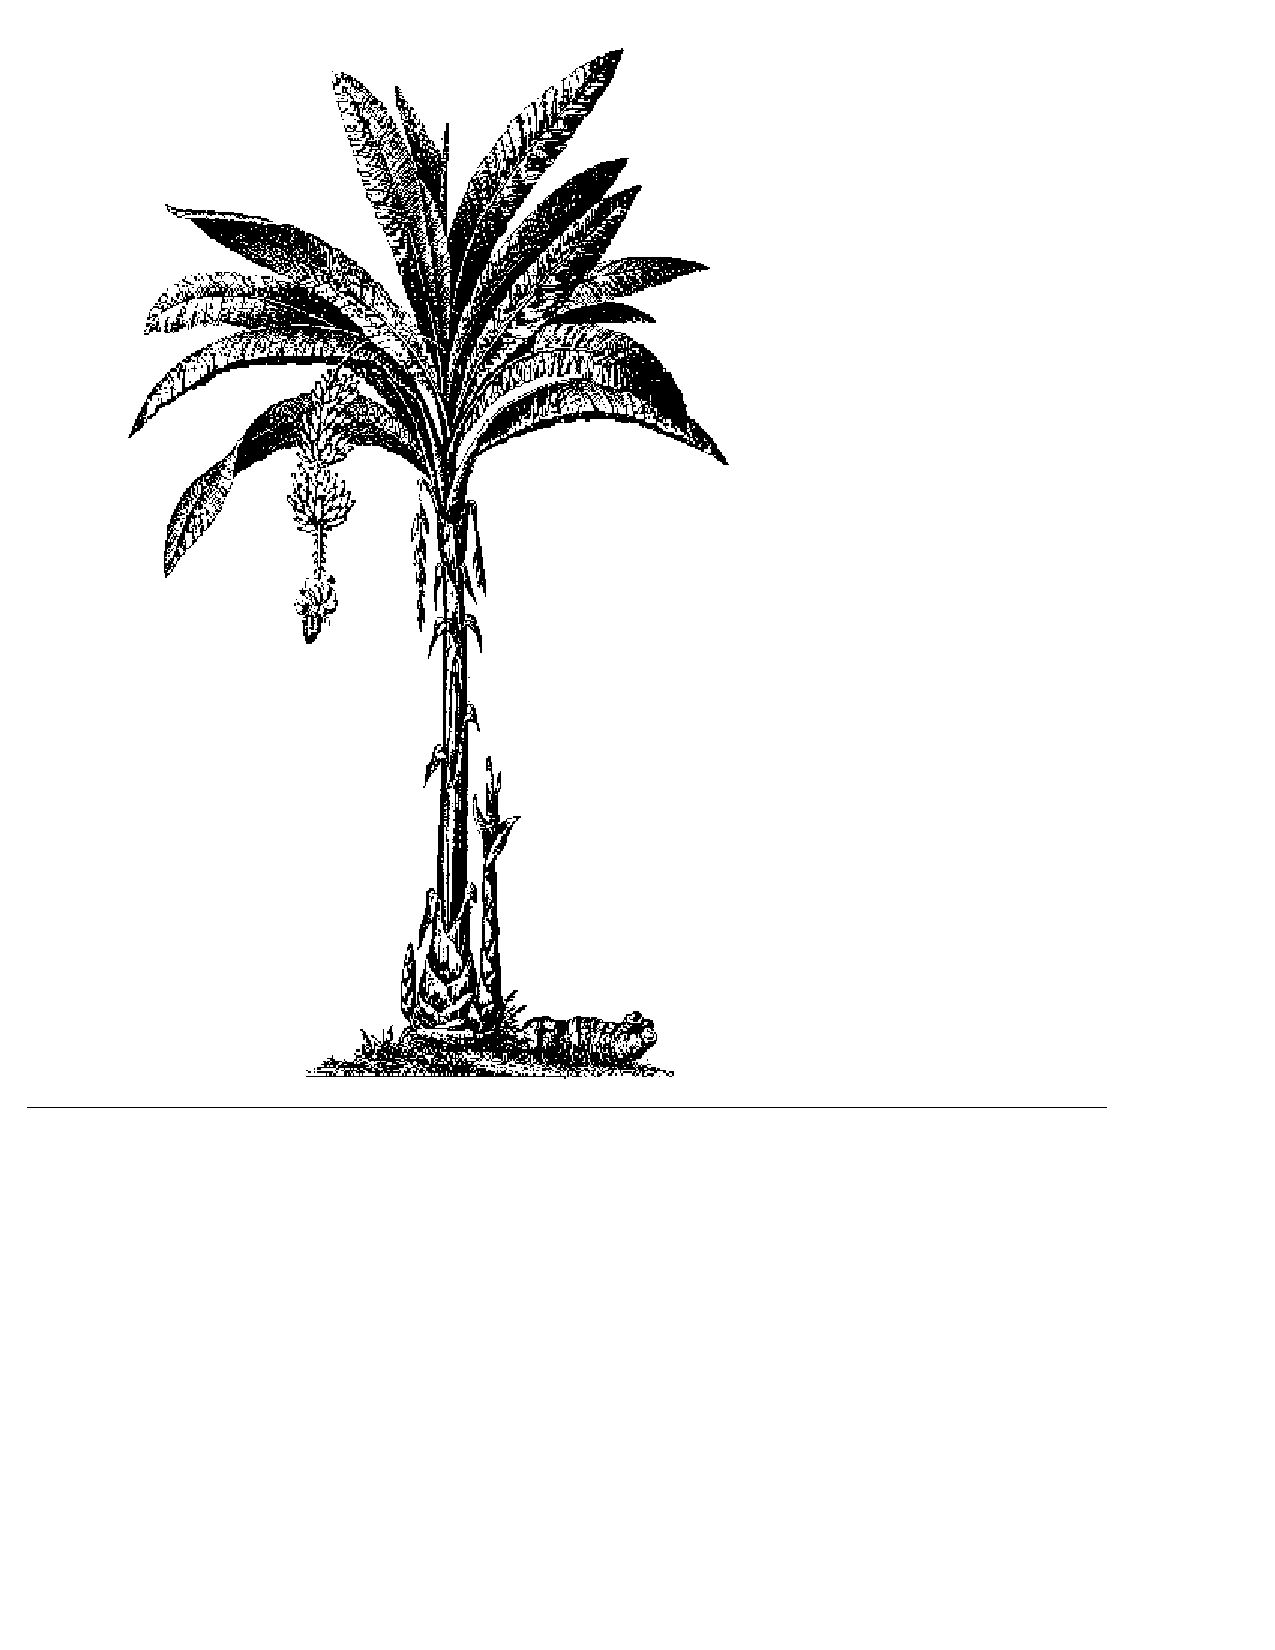
\includegraphics[scale=.4,ext=.pdf,%
%    angle=101,trim=-50 245 125 125]{palm}}}%
%    \makelth{Homea}{\Lheader{\usebox{\Lpalms}}}%
%    \end{verbatim}
%
%    \subsection{Marginal material}
%    The left and right margins may also contain a box of text.  This is placed in
%    |\Lmargin| or |\Rmargin|.   The size of the  margin is automatically calculated from
%    the box size.  The box is placed a very small distance from the  edge
%    of the paper (10pt), and the margin gap from the box to the text box of
%    the letter is set to be 10pt as well.  
%
%    In some cases, the header and footer margins may be too small when
%    fitted to the boxed-up header and footer items.  For this reason,
%    four commands allow the headers and footers to have a given minimum
%    size.  These commands are |minhead=xxpt| (minimum size for header of
%    non-letterhead page; xxpt is a dimensional value such as |5in| or
%    |12pt|), |MinHead=xxpt| (minimum size for header of
%    letterhead page), |minfoot=xxpt| (minimum size for footer of
%    non-letterhead page) and |MinFoot=xxpt| (minimum size for footer of
%    letterhead page).  These ensure that the headers and footers have given
%    minimum sizes.  
%
%    \subsection{Graphical objects}
%    Here is a step-by-step description of the process of incorporating a
%    graphical object:
%    \begin{itemize*}
%    \item \textbf{Insert the object:}
%      Insert the graphical object into the document (|\includegraphics|).
%    \item \textbf{Check object:}
%      Ensure that the graphical object is included correctly.  Prior to
%      attempting to use |newlfm| to print the object, ensure that
%      |\includegraphics| has inserted the \info{} correctly.  Using the
%      |\fbox| specification to allow the box edges to be examined carefully,
%      print the boxed \info{} to ensure that the object is correctly
%      specified, and that the size is correct.  If the appearance is
%      appropriate, use the wide range of options in the |\includegraphics| 
%      command (|clip|, |view|, |bb|, |trim|, |size|, etc.) to make the
%      object appear as you wish it.
%    \item \textbf{Use object:} 
%      Use the resulting trimmed, clipped and selected object in one of the
%      commands for inclusion in a |newlfm| letter or memo.
%    \item \textbf{Usage tip:} 
%      Run \LaTeX{} twice to ensure that dimensions are correctly interpreted. 
%    \end{itemize*}
%
%    \subsection{Example use of external object:}
%    Here is an example of the inclusion of an external object and its use
%    in constructing a letterhead page.  A |\newsavebox| is constructed and
%    used to store the object.  |\includegraphics| is used to insert the
%    object.  If commands to produce a .ps file are used (|latex file|,
%    |dvips file|), \LaTeX\ will search for a file with the .ps or .eps
%    suffix.  If commands to produce a .pdf file are used (|pdflatex file|),
%    \LaTeX\ will search for a file with the .pdf suffix.  For
%    flexibility, omit the suffix.
%    \begin{verbatim}
%    \newsavebox{\Logob}%
%    \sbox{\Logob}{\parbox[t]{\vdim}{\includegraphics[scale=.8]{wulogo3}}}%
%    \makeaddress{PAT}{%
%    \name{Paul A. Thompson, Ph.D.}%
%    \addr{\parbox[b]{2.65in}{Washington University School of Medicine \\%
%    at Washington University Medical Center \\ Box 8067, 660 S. Euclid \\%
%    St. Louis, MO    63110-1093}}%
%    \phone{(314) 747-3793}\fax{(314) 362-2693}\email{paul@wubios.wustl.edu}%
%    }
%    \makeaddress{GRQ}{%
%    \name{Roger Q. Grollier}%
%    \addr{\parbox[b]{2.65in}{25 N. Eastwind Rd.\\Westend, OH 43431}}%
%    \phone{(412) 555-2324}\fax{(412) 555-6923}\email{roger@starlik.com}%
%    }
%    \makeletterhead{WULHb}{%
%    \setadrfr{\adrPAT}\Lheader{\usebox{\Logob}}%
%    \Rheader{{\large\bf Division of Biostatistics}}\rheader{\@name@fr}%
%    \lheader{Page \thepage}\Lfooter{\smallform}\closeline{Sincerely yours,}%
%    }%
%    \end{verbatim}
%
%    The two |makeaddress| specificiations set up wrapper commands (see
%    Section \ref{sect:wrapper} below) which  encapsulate the relevant
%    information.  The |\setadrfr| specification in the example converts the
%    address information in |\adrPAT| from neutral to ``from-address''
%    formats.  This can also be done using the wrapper ID specification, where it
%    would be stated as |\setadrto{\fixadr{GRQ}}|, where the |\fixadr|
%    specification converts the wrapper ID to the wrapper internally.    
%
%    In a letter, this is used as:
%    \begin{verbatim}
%    \documentclass[dvips]{newlfm} 
%    \lthWULHb\setadrto{\adrGRQ}
%    \begin{document}
%    \begin{newlfm}
%    ....
%    \end{verbatim}
%    For this example, the object found in |wulogo3| was boxed up using
%    the |\sbox| specification.  It will be placed in the
%    left section of the header block for the letterhead page.  The logo was
%    examined earlier to ensure that it
%    is printed exactly as required.
%
%    \paragraph*{Usage tip:}
%    Examine the example of the inclusion of the graphical object above
%    carefully.  Note that all lines are terminated with the comment
%    character ``\verb|%|''.  All wrapper macros should be constructed in
%    this manner, to ensure that no blank spaces are inadvertently placed in the
%    wrapper macro \textbf{between commands}, other than those placed within
%    a command (for instance, the |\addr| command has blanks).  The wrapper
%    macros should not have blanks around commands, either before the start
%    of a command or after the end of one. The wrappers are ``unpacked'' 
%    during active text construction, and the presence of blanks can
%    result in odd, difficult-to-trace minor justification anomalies.  In
%    many cases, the author has found it helpful to ensure that all lines in
%    the wrapper addresses and terms are terminated with the ``\verb|%|''
%    comment character, to ensure that end-of-line characters are not
%    translated into hard-to-detect space characters.
%
%    \subsection{Including a pre-set sheet as background}
%    In some cases, the letterhead or pre-set form is to be included as a full sheet of
%    letterhead information.  In this case, the pre-set form may be designated
%    using the command |Background| (for letterhead form for the first page), and |background|
%    (for pre-set form for subsequent pages after the first page).  The form to be
%    included should be set up as a valid graphical object.  In the case of the use of
%    the |pdflatex| process, it should be set up as a |.pdf| form, and in the case of
%    |latex| processing, it should be set up as a valid |.ps| form, using the
%    encapsulated PostScript approach with a valid bounding box.
%
%    \subsection{Blank block printing commands}
%    In some cases, the user wishes to use the included graphical objects to
%    size the header and footer areas (covered in Section \ref{sect:lhead}
%    below), and then not actually print the  objects
%    {\itshape per se}.  For instance, the letter may be printed on letterhead
%    stock, using the letterhead objects included to size the letter.  In that
%    case, the options shown in \tabr{blankopt} are available to blank out the various
%    parts of the letterhead \info{} after it is used to set margin sizes. 
%
%    \tabsetx{4}{Options for blanking}{blankopt}
%    \begin{center}
%    \begin{tabular}{llllll}
%    \hline 
%    \hdr{Option} & \hdr{Blanks \ldots} & \hdr{Option} & \hdr{Blanks \ldots} &
%    \hdr{Option} & \hdr{Blanks \ldots}  \\ \hline 
%    |blankheader| & |r,l,cheader| &
%    |blankfooter| & |r,l,cfooter| &
%    |blanklmargin| & |lmargin| \\
%    |blankrmargin| & |rmargin| &
%    |Blankheader| & |R,L,Cheader| &
%    |Blankfooter| & |R,L,Cfooter| \\
%    |Blanklmargin| & |Lmargin| &
%    |Blankrmargin| & |Rmargin| &
%    |Blankall| & All upper-case  \\
%    |blankall| & All lower-case &
%    |Blank|    & All \\
%    \hline
%    \end{tabular}
%    \end{center}
%        
%    \section{The letter database}
%    \label{sect:wrapper}
%    \subsection{Letter database {\tt letrinfo.tex}}
%    \Info{} for letters may be stored in a file.  The default name of the 
%    file is |letrinfo.tex|.   This file
%    stores \info{} in two ways: unconditionally and conditionally.  The
%    conditional \info{}, such as lists of addresses associated with
%    names, is stored in ``wrappers'', which carry the \info{} from
%    the file |letrinfo.tex| to each letter.  The
%    information stored in the letter database file |letrinfo.tex| is letter
%    information (i.e., |\name{Paul Thompson}|, |\PhrPhone{Telephone #}|). 
%  
%    Several types of \info{} are stored in the file |letrinfo.tex|.  These
%    different types of \info{} may be stored in several ways.  It may be
%    stored unconditionally, by placing it into the file |letrinfo.tex|.
%    All \info{}, used in the order listed, will be available for all letters.  
%    
%    Most \info{} is not unconditional, however.  For this reason, the \info{}
%    will almost always be stored in address ``wrappers''.  This
%    includes \info{} about the ``from'' person, as this \info{} may
%    change based on the style of letter, etc.  The \info{} may be divided into
%    three different types, and is thus placed into three types of
%    wrapper commands. 
%
%    \subsection{Address \info{}}
%    \label{page:wrapc}
%    Address \info{} is stored in an address wrapper.  The address wrapper
%    has an wrapper ID and a body. The wrapper is set up using the command:
%    \begin{verbatim}
%    \makeaddress{IDENT}{stuff}. 
%    \end{verbatim} 
%    The wrapper ID is |IDENT|.
%    This makes a wrapper for 
%    addresses, |\adrIDENT|.  Commands placed in the wrapper are then carried into 
%    the document when the wrapper command is placed in the letter as:
%    \begin{verbatim}
%    \begin{document}
%    \setadrto{\adrIDENT}
%    \setadrfr{\adrOTHID}
%    \begin{newlfm}
%    ......
%    \end{verbatim}
%    Note that the wrapper command is placed after |\begin{document}| and
%    before |\begin{newlfm}|.
%    All items entered into the |IDENT| wrapper are then activated in that
%    particular document.  This enables \info{} to be centrally stored in the
%    |letrinfo.tex| file, and used in each actual letter. 
%
%    The wrappers may also be indicated using the  |newlfmP|
%    key-value specification:
%    \begin{verbatim}
%    \begin{document}
%    \newlfmP{addrt=IDENT,addrf=OTHID}
%    \begin{newlfm}
%    ......
%    \end{verbatim}
%    This also sets up |IDENT| as the ``to'' address and |OTHID| as the
%    ``from'' address.  
%
%    Wrapper commands have two parameters.  
%    \begin{itemize*}
%    \item The wrapper ID is the first parameter in the |\makeaddress|
%    specification.  The wrapper ID is used to set up
%    a new command |\adrIDENT|, and is used in many other places by itself.
%    In general, a simple identifier is best (i.e., addressee's initials).  
%    \item The actual items are placed in the second set of braces.  The
%    wrapper ID is case-sensitive.
%    Whatever is placed there is used in the command, and carried along
%    whenever it is used.  The user may choose to place a wide variety of
%    information in the wrapper.  Commands usually used in address wrapper commands
%    are shown in \tabr{adrtoc}.  
%    \end{itemize*}
%
%    The address \info{} for a certain individual usually does not change
%    from letter to letter, although different persons are used in different
%    letters.  By using address info{} wrappers, the \info{} can 
%    be handled and used easily with the single wrapper command.  This
%    information  may be used for either the sender or the addressee for the
%    letter.   
%
%    \paragraph{Designating a sender:} To use the address information for 
%    the sender or ``from-person,'' use the |\setadrfr| command or the
%    |addrf| term in the |newlfmP| command:
%    \begin{verbatim}
%    \setadrfr{\adrPAT} 
%    \setadrfr{\fixadr{PAT}}
%    \newlfmP{addrf=PAT}
%    \end{verbatim}
%    This sets up the information in the |PAT| wrapper to be 
%    placed in the ``from'' blanks of the letter. 
%    If the wrapper ID is used in the |\setadrfr| command, the |\fixadr| command
%    converts the wrapper ID to the correct form.
%    \paragraph{Designating a recipient:} To use the address 
%    information for the recipient, use the |\setadrto| command or the 
%    |addrt| term in the |newlfmP| command:
%    \begin{verbatim}
%    \setadrto{\adrPAT} 
%    \newlfmP{addrt=PAT}
%    \setadrto{\fixadr{PAT}}
%    \end{verbatim}
%    This would set up the information in the |PAT| wrapper to be 
%    placed in the ``to'' blanks of the letter.
%
%    \subsection{Letterhead \info{}}
%    Letterhead \info{} is stored in a letterhead wrapper.  The wrapper is 
%    prepared using the command:
%    \begin{verbatim}
%    \makeletterhead{LIDENT}{stuff}
%    \end{verbatim}
%    The wrapper usually contains \info about the header, footer and margin
%    objects, which are used to set up the letterhead.  This wrapper is
%    used like the |\makeaddress| command.
%    In many cases, the return address of the letter author is set up in the 
%    letterhead wrapper, because this does not change:
%    \begin{verbatim}
%    \makeletterhead{HomeA}{%
%    \rheader{this}%
%    \setadrfr{\adrPAT}%
%    }%
%    \end{verbatim}
%
%    \subsection{Signature \info{}} 
%    Signature \info{} is stored in an signature wrapper.  The wrapper is 
%    prepared using the command
%    \begin{verbatim}
%    \makesignature{SIDENT}{stuff}  
%    \end{verbatim}
%    This wrapper is used like  the |\makeaddress| command.
%    The \info{} shown in \tabr{sigsc} is usually included in the 
%    |\makesignature| wrapper.
%
%    \tabsetx{6}{Signature Commands}{sigsc}
%    \begin{center}
%    \begin{tabular}{llll} \hline
%    \hdr{Command} & \hdr{Use}& \hdr{Command} & \hdr{Use} \\ \hline
%    |\signature| & Boxed-up signature & |\signame| & Printed name \\ 
%    |\closeline| & Letter closing line \\ \hline
%    \end{tabular}
%    \end{center}
%
%    In some cases, multiple signatures are required.  These are listed in a
%    command |\siglist|:
%    \begin{verbatim}
%    \siglist{AAA,BBB,CCC}
%    \end{verbatim}
%    In this case, three signatures are printed.  By default, they are
%    printed in a left-justified column.  To print them in a row, use
%    |\sigacross{2}| to indicate the number of signature blocks printed in
%    each row (the maximum number is 4).  Each signature is printed in a
%    block of the height and width of the largest signature block.  For this
%    approach, the letter will look odd and unbalanced if signatures are of
%    different sizes. The user must ensure that all signatures are of the same
%    size, as the program cannot ensure this.  Additionally, each signature
%    wrapper is unpacked to determine closing line and printed name. 
%    Spacing between signature block columns is set by |\sigskipcolumn|, and
%    spacing between signature block rows is set by |\sigskiprow|.
%
%    \subsection{Closing \info{}} 
%    Other closing items may be included in the letter itself, in the
%    file |letrinfo.tex|.  These include the following:
%
%    \tabsetx{6}{Closing commands}{eolc}
%    \begin{center}
%    \begin{tabular}{llllll} \hline
%    \hdr{Command} & \hdr{Usage} & \hdr{Command} & \hdr{Usage} & 
%    \hdr{Command} & \hdr{Usage} \\ \hline
%    |\cclist| & Routing list &
%    |\encllist| & Enclosures list &
%    |\initials| & Sender initials \\
%    |\faxmssg| & FAX cover message &
%    |\psitem| & Ps line &
%    |\ppsitem| & Pps line \\
%    |\pppsitem| & ppps line &
%    |\re| & re line &
%    |\subre| & Second re line \\ \hline
%    \end{tabular}
%    \end{center}
%
%    \subsection{Setting up wrapper macros}
%    \paragraph{File {\tt letrinfo.tex}:}
%    \begin{verbatim}
%    \makesignature{PT}{\newsavebox{\Signature}
%    \sbox{\Sigx}{\includegraphics[bb=16 9 597 784,viewport=180 350 400
%    425,scale=6,%
%    height=.6in,width=1.375in,clip]{sigfile}%
%    }%
%    \signature{\usebox{\Sigx}}%
%    \signame{\raisebox{.5in}{\parbox[t]{5in}{Paul A. Thompson \\%
%    Associate Professor \\ Div.  Biostatistics \\%
%    Washington University School of Mecicine}}}%
%    }%
%    \makeaddress{JS}{\name{Joe Smith}%
%    \address{12 Center Street \\ Greenville, OH 55555}%
%    \phone{(312) 333-4444}\greet{Dear Joe,}%
%    }%
%    \makeaddress{PAT}{\name{Paul A. Thompson, Ph.D.}%
%    \addr{\parbox[b]{2.75in}{Washington University School of Medicine \\%
%    Box 8067, 660 S. Euclid \\ St. Louis, MO    63110-1093}}%
%    \phone{(314) 747-3793}\fax{(314) 362-2693}%
%    }%
%    \newsavebox{\Logob}%
%    \sbox{\Logob}{\parbox[t]{\vdim}{\includegraphics[scale=.8]{wulogo3}}}%
%    %
%    \makeletterhead{WULHa}{%
%    \sigPT%
%    \Lheader{\usebox{\Logob}}\setadrfr{\adrPAT}%
%    }%
%    \end{verbatim}
%
%    \paragraph{Use in a letter:}
%    \begin{verbatim}
%    \documentclass[american]{newlfm}
%    \newlfmP{letrh=WULHa,addrt=JS}
%    \begin{document} 
%    \begin{newlfm}
%    ...
%    \end{newlfm}
%    \end{document}
%    \end{verbatim}
%
%    This letter will be addressed to Joe  Smith, using the letterhead stored
%    in |WULHa|.  The signature is taken from signature wrapper |PT|, which is carried
%    along with the letterhead wrapper |WULHa|.
%    In this way, the letters can be addressed to Joe Smith very easily, by
%    merely including the file |letrinfo.tex| on the \LaTeX{} path, and
%    including the wrapper as shown above in the file.  Although initials for
%    the recipient need not be used as the wrapper identifier tag, this is
%    convenient and makes the wrapper designation easy to do.
%
%    The wrapper commands may be used in a nested fashion.  Consider this
%    sequence: 
%    \begin{verbatim}
%    \makeaddress{Main}{\name{Paul A. Thompson}%
%    \addr{WU School of Medicine}}%
%    \makeaddress{YouA}{\adrMain \name{Love A}
%    \addr{Whereever you are}}%
%    \makeaddress{YouB}{\adrMain \name{Love B}%
%    \addr{The White House}}%
%    \end{verbatim}
%
%    In this case, the \info{} in |adrmain| is carried into the wrappers
%    |adrYouA| and |adrYouB| and is available there.  This is similar to  the
%    concept of inheritence in object-oriented programming.
%
%    \subsection{Multiple information datasets}
%    By default, |newlfm| looks for a file |letrinfo.tex| on the \TeX\
%    path.  If this file is found, it is read in during the initialization
%    process of the  |newlfm| environment.  If an alternative file is
%    needed, it may be indicated using the command
%    |\InfoFileName{check.tex}|.  This file will then be used in place of
%    |letrinfo.tex|. 
%
%    \subsection{Rules for use of wrapper IDs}
%    The wrapper IDs used to construct the letterhead database can be used in two
%    different ways.  First, the address or letterhead wrappers may be used
%    by themselves as |\adrSETA| or |\ltrSETB|.  Second, the wrapper IDs may
%    be used in many situations without the |\adr|.  Here are the general
%    rules for usage:
%    \begin{enumerate}
%    \item The wrapper macro |\adrXXX| may be used at any point in a letter.
%    To properly set up margins, it should be used  as |\setadrto{\adrXXX}|
%    and |\setadrfr{\adrXXX}| (used to convert neutral address
%    information into to-address and from-address information) prior to the
%    |\begin{newlfm}| command.  This 
%    will  ensure that proper spacing decisions are made.  The
%    |\doletter| construction also uses this form of wrapper (note: this
%    command is now obsolete - please use |\oneletter| as described below).
%    \item Wrapper IDs can be used as |\setadrto{\fixadr{XXX}}| to
%    convert neutral addresses to to-addresses and from-addresses (again,
%    prior to |\begin{newlfm}|.
%    Additionally, |\oneletter{XXX}| is used to send a form letter to
%    address |XXX|, |\multletter{XXX,YYY,ZZZ}| to multiple addresses, and
%    |\newlfmP{addrt=AAA,addrf=BBB}| are used to convert addresses using the
%    |\newlfmP| mechanism.
%    \end{enumerate}
%
%    \section{Form letters}
%    \label{sec:form}
%    The use of the address wrapper commands makes it very easy to set up form
%    letters.  \verb|newlfm| has a simple approach to form letters, using two
%    commands:
%    \begin{itemize*}
%    \item \verb|\letterbody|: This command is used to set up the body of the
%    letter.  The body is the text of the letter.  When you set up the body,
%    it is very easy to further customize the letters by setting up commands
%    within the letter.
%    \item \verb|\oneletter|: This is the  command to print the different 
%    letters.  The command has a mandatory argument of the label of the
%    ``to'' address. 
%    \item \verb|\multletter|: This command allows the use of a list of
%    address wrapper labels that will all be used to print a form letter.  The
%    address wrapper labels must all be separated by the comma (``,'').  When
%    printing form letters in this manner, specific tailoring can only be
%    done if the tailoring information is included in the  address wrapper.
%    Thus, this can be used to print any number of identical letters, or
%    letters which have been tailored or modified using information in the
%    address wrappers.
%    \end{itemize*}
%
%    \subsection{Example form letter}
%    Here is an example of the use of the form-letter commands.  In this
%    example, the two wrapper commands \verb|\adrAA| and \verb|\adrBB| can be
%    used to address letters which are both the same to the persons listed
%    in these wrappers:
%    \begin{verbatim}
%    \letterbody{This is an example of a form letter. \tailor End of the letter.}%
%    \newcommand{\tailor}{First special version.}
%    \oneletter{AA}
%    \letterbody{This is a second example of a form letter, but this approach does not allow for 
%    individualization.  It is being sent to \printnameto.}
%    \multletter{AA,BB}
%    \renewcommand{\tailor}

%     {Second special version.}
%    \oneletter{BB}
%    \end{verbatim}
%
%    \section{Printing envelopes and labels}
%    \label{sec:env}
%    |newlfm| includes a set of commands which print labels.  Some invoke the functionality of the
%    |envlab| package.  To use this functionality, follow these steps:
%    \begin{enumerate*}
%    \item Ensure that |envlab| is properly installed in your \TeX
%      installation, and that the installation database has been properly
%      refreshed.  This will ensure that \LaTeX{} can find the files.
%    \item Use the option |useenvlab| on the command line:
%    \begin{verbatim}
%    \documentclass[useenvlab]{newlfm}
%    \end{verbatim}
%    This will issue the |\makelabels| command at the start of the run, issue
%    the |\startlabels| command at the end of the run, insert the
%    ``from-address'' and ``to-address'' into appropriate structures for
%    |envlab| and otherwise complete the printing of the envelope using
%    internal information.
%    \item Options which are needed for |envlab| may also be entered into the
%    \LaTeX\ command line, just as with any normal use of |envlab| during any
%    \LaTeX.
%    \item Several types of Avery labels may be used.  The specifications
%    for Avery labels 5160, 5161, 5162, 5163 and 5164 are pre-set in
%    |newlfm|.  These are summarized in the table below.
%
%    \tabsetx{6}{Label definitions}{labels}
%    \label{tab:d}
%    \begin{center}
%    \begin{tabular}{lrrlrrrr} \hline
%    Option & Ht & Wt & t & l & Btw & Col & Row \\ \hline
%    Avery5160 & 1 & 2.75 & .5 & .19 & .16 &3 & 10 \\
%    Avery5161 & 1 & 4.19 & .5 & .16 &.19 &2 & 10 \\
%    Avery5162 & 1 & 4.19 & .83 & .16 &.19 &2 &  7 \\
%    Avery5163 & 1 & 4.19 & .5 & .16 &.19 &2 & 5  \\
%    Avery5164 & 1 & 4.19 & .5 & .16 &.19 &2 &  3 \\ \hline
%    \end{tabular}
%    \end{center}
%
%    \item Several options exist for address selection during label printing.  The default
%    is |labto|,  in which the ``to-address'' only is printed.  If
%    |labrowfrto| is selected, both ``from-address'' and ``to-address'' are
%    printed in a row:
%    \begin{verbatim}
%    From: Paul A. Thompson     To: George W. Bush
%          25 Signal Hill Blvd      1400 W. Turkey Rd.
%          Belleville, IL 62223     Crawford, TX 49281
%    \end{verbatim}  If
%    |labcolfrto| is selected, both ``from-address'' and ``to-address'' are
%    printed in a column:
%    \begin{verbatim}
%    From: Paul A. Thompson     
%          25 Signal Hill Blvd  
%          Belleville, IL 62223
%    To:   George W. Bush
%          1400 W. Turkey Rd.
%          Crawford, TX 49281
%    \end{verbatim}
%    The user is responsible for ensuring that the label printing options
%    can fit on the label selected; Avery5160 is generally suitable only for
%    |labto|, but other choices can fit on other labels. 
%    \item Other printing sizes may be selected during label printing using
%    |labsize=\size|: 
%    \begin{verbatim}
%    labsize=\small
%    \end{verbatim}
%    \end{enumerate*}
%
%    \section{Miscellaneous topics}
%    \subsection{Lines}
%    By default, |newlfm| demarcates the header and footer sections with
%    lines.  These may be eliminated using the commands |noHeadline|, |noFootline|,
%    |noLines|  (for the letterhead page), and |noheadline|, |nofootline|, 
%    |nolines| (for subsequent pages).  These commands eliminate lines in either the 
%    letterhead page or the non-letterhead page.  Line widths may be set as
%    well, using the commands |Headlinewd| (sets head linewidth for
%    letterhead page), |headlinewd| (sets head linewidth for
%    non-letterhead page), |Footlinewd| (sets foot linewidth for
%    letterhead page), and |footlinewd| (sets foot linewidth for
%    non-letterhead page).  These final four commands issued either in the
%    command line or in the |newlfmP| commands as:
%    \begin{verbatim}
%    \newlfmP{Headlinewd=.5pt,footlinewd=.75pt}
%    \end{verbatim}
%    If a line width is set to 0pt, the line is not printed.
%    \subsection{Printing information on additional pages}
%    In many letters, the letterhead page is to be followed by additional information
%    on additional, non-letterhead pages.  This may be done using the
%    |\restlettera{text}|,  |\restletterb{text}|,  |\restletterc{text}|,
%    |\restletterd{text}|, and  |\restlettere{text}| 
%    commands.  Following the issuance of the signature, a |\newpage| command is
%    issued, and the information contained in the 
%    |\restlettera{text}|,  |\restletterb{text}|,  |\restletterc{text}|,
%    |\restletterd{text}|, and  |\restlettere{text}|  blocks are printed.  These 
%    need not be used sequentially.
%    These blocks must not have spaces.  If paragraphs are to be used, use |\paragraph|
%    to force the new paragraph without an actual blank line.  In addition, extra material
%    in each section is limited to a single page.  The letterhead rules for the extra
%    pages follow the rules for the non-first page.
%    \subsection{Setting the date}
%    The date for the letter is set to be the date upon which the letter is
%    typeset.  To change the date, use |\dateset{May 20, 1974}| (feel free
%    to use other dates as needed).  
%    |\dateset{\today}| prints today's date.
%
%    \subsection{Language option definitions:}  
%    \label{sec:othlang}
%    These options define the language for the letter.  These macros are not 
%    frequently manipulated.  Basically, the strings defined here
%    set up the printing of structural elements of a memo or letter, such as
%    the ``From'' or ``To'' strings.  
% 
%    These terms are used at various points in printing letters and memos.
%    They are American terms; your mileage may vary.  Inclusion of other
%    terms is encouraged, especially when another language group is served.
%    This may be done as follows:
%    \begin{enumerate}
%    \item Change the letters ``am'' to either ``fr'' for French, ``gr'' for
%    German, ``en'' for English, ``ot'' for other or ``pl'' for pig-Latin.  If
%    you feel that I have unfairly cast disrespect on your language, feel free 
%    to add appropriate code in the section above for your language.  Change 
%    phrases in the following terms to the appropriate terms for the language
%    in question:
%    \begin{verbatim}
%    \newcommand{\@am@phr}{%
%      \renewcommand*{\@fax@cover@line}
%          {FAX Cover Page}% 
%      \renewcommand*{\@fax@page@count}
%          {FAX Page Count}%
%      \renewcommand*{\@fax@phr}{FAX}%
%      \renewcommand*{\@pager@phr}{Pager}%
%      \renewcommand*{\@doc@phr}{Document}%
%      \renewcommand*{\@phn@phr}{Phone}%
%      \renewcommand*{\@email@phr}{E-mail}%
%      \renewcommand*{\@re@phr}{Re}%
%      \renewcommand*{\@subre@phr}
%          {\ensuremath{\mathrm{Re}_2}}%
%      \renewcommand*{\@cc@phr}{cc}%
%      \renewcommand*{\@ps@phr}{Ps}%
%      \renewcommand*{\@m@phr}{Message}%
%      \renewcommand*{\@pps@phr}{Pps}%
%      \renewcommand*{\@ppps@phr}{Ppps}%
%      \renewcommand*{\@encl@phr}{Encl}%
%      \renewcommand*{\@pager@phr}{Page}%
%      \renewcommand*{\@hnto@phr}{To}%
%      \renewcommand*{\@hnfr@phr}{From}%
%    }
%    \end{verbatim}
%    \item Use file |extracd.tex| to store the new commands.  This file
%      should be placed in the same subdirectory as |newlfm.cls|.  When the
%      program executes, it includes the file if it is found.  
%    \item Use the appropriate option to include the correct code.
%    \end{enumerate}
%    \subsection{Printing the address information}
%    The |newlfm| package prints a variety of address \info{} in
%    specific ways which are appropriate and standard for letters.  In some
%    cases, you may wish to print other \info{} from the addresses in more
%    flexible ways.  For this purpose, certain printing macros are defined.
%    These are shown in \tabr{printcom}.
%
%    \tabsetx{4}{Printing address information}{printcom}
%    \begin{center}
%    \begin{tabular}{lllll}
%    \hline 
%    Select & Command & Item & Command & Item  \\ \hline 
%    ``To'' & |\printnameto| & Name &
%    |\printaddrto| &  address \\
%    & |\printphoneto| & phone &
%    |\printphoneato| &  phone A \\
%    & |\printphonebto| &   phone B &
%    |\printphonecto| &   phone C \\
%    & |\printphonedto| &   phone D &
%    |\printphoneoto| &   phone O \\
%    & |\printphonehto| &   phone H &
%    |\printpagerto| &  pager \\
%    & |\printfaxto| &  FAX &
%    |\printgreetto| &  greeting \\
%    & |\printemailto| &  email &
%    |\printemailbto| &  email \\
%    & |\printemailcto| &  email C  &
%    |\printlnameto| &  last name \\
%    |\printfnameto| &  first name \\
%    ``From'' & |\printnamefrom| & name &
%    |\printaddrfrom| &   address \\
%    & |\printphonefrom| &   phone  &
%    |\printphoneafrom| &   phone A \\
%    & |\printphonebfrom| &    phone B &
%    |\printphonecfrom| &    phone C\ \\
%    & |\printphonedfrom| &    phone D &
%    |\printphoneofrom| &    phone O \\
%    & |\printphonehfrom| &    phone H &
%    |\printpagerfrom| &   pager \\
%    & |\printfaxfrom| &   FAX &
%    |\printgreetfrom| &   greet \\ing 
%    & |\printemailfrom| &   email &
%    |\printemailbfrom| &   email \\
%    & |\printemailcfrom| &   email C &
%    |\printlnamefrom| &   last name \\
%    & |\printfnamefrom| &   first name \\
%    \hline
%    \end{tabular}
%    \end{center}
%    
%    These commands can be issued in any letter to print the \info{} for the
%    particular address component.
%
%    \subsection{Cellophane-window envelopes}
%    Letters are sometimes set up to be printed for a cellophane-window
%    envelope.  Using this approach, the ``to-address'' must be placed into
%    a specific orientation.  In |newlfm|, this is particularily
%    challenging, as the class attempts to grant users great flexibility.
%
%    In |newlfm|, users can specify the use of a cellophane-window
%    envelope.  The |cellowindow| option specifies this choice.  The
%    ``to-address'' block is positioned down from the top (using |cellodown|
%    to specify the length down; default =  2.5 inches) and left from the side (using |celloleft|
%    to specify the length from the left; default = 1 inch).  If the user specifies the
%    printing of a ``from-address'' and a date, it may not be possible to
%    print the ``to-address'' in the correct location; in this case, the
%    user should carefully examine the log and the output screen to
%    determine if the specified locations can be used in the context of
%    other options.  
%    The user can also specify the height and width of the ``to-address''
%    block as |cellowidth| (default = 4 inches) and |celloheight| (default =
%    1 inch). 
%
%    \subsection{Examples}
%    |newlfm| includes a large number of examples specified as |test1.tex|
%    through |test12.tex|.  These examples all specify their options using
%    the |newlfmP| mechanism.  Each file is also set up using the
%    |\documentclass| specification, on |test1alt.tex| through
%    |test8alt.tex|.  When preparing examples, both |pdflatex| and |latex| are
%    both used to prepare examples.
%
%    \newcommand{\pdfLaTeX}{\texttt{pdf}\LaTeX}
%    \subsection{\LaTeX\ vs. \pdfLaTeX}
%    \pdfLaTeX\ is becoming more and more common in document production in
%    the \TeX\ family.  It is not the standard yet, and there remain tools
%    which work only in the \LaTeX\ system (i.e., |pstricks|).  
%
%    The author uses |.eps| files, constructed to ensure that the bounding
%    box accurately encapsulates the active text area of the |.eps| figure.
%    Each of the figures was then converted to |.pdf| encoding using
%    |GSview|.  However, the bounding box in the |.pdf| files does not seem
%    to act to crop the image in the same manner.  Using the same code for
%    both \pdfLaTeX\ and \LaTeX\ processing does not result in the same
%    appearance of the output page.  
%
%    For this reason, functionality of H. Oberdiek's |ifpdf.sty| file is
%    included in |newlfm|.  This tool allows one option to be performed
%    when \pdfLaTeX is used for processing, and another option to be
%    executed in the \LaTeX\ environment.  Use of this tool is illustrated in the
%    |letrinfo.tex| file included in the |newlfm| package.
%    
%    Here is an example:
%    \begin{verbatim}
%    \newsavebox{\Lpalme}%
%    \ifpdf
%    \savebox{\Lpalme}{\parbox[t][1in][t]{2in}%
%    {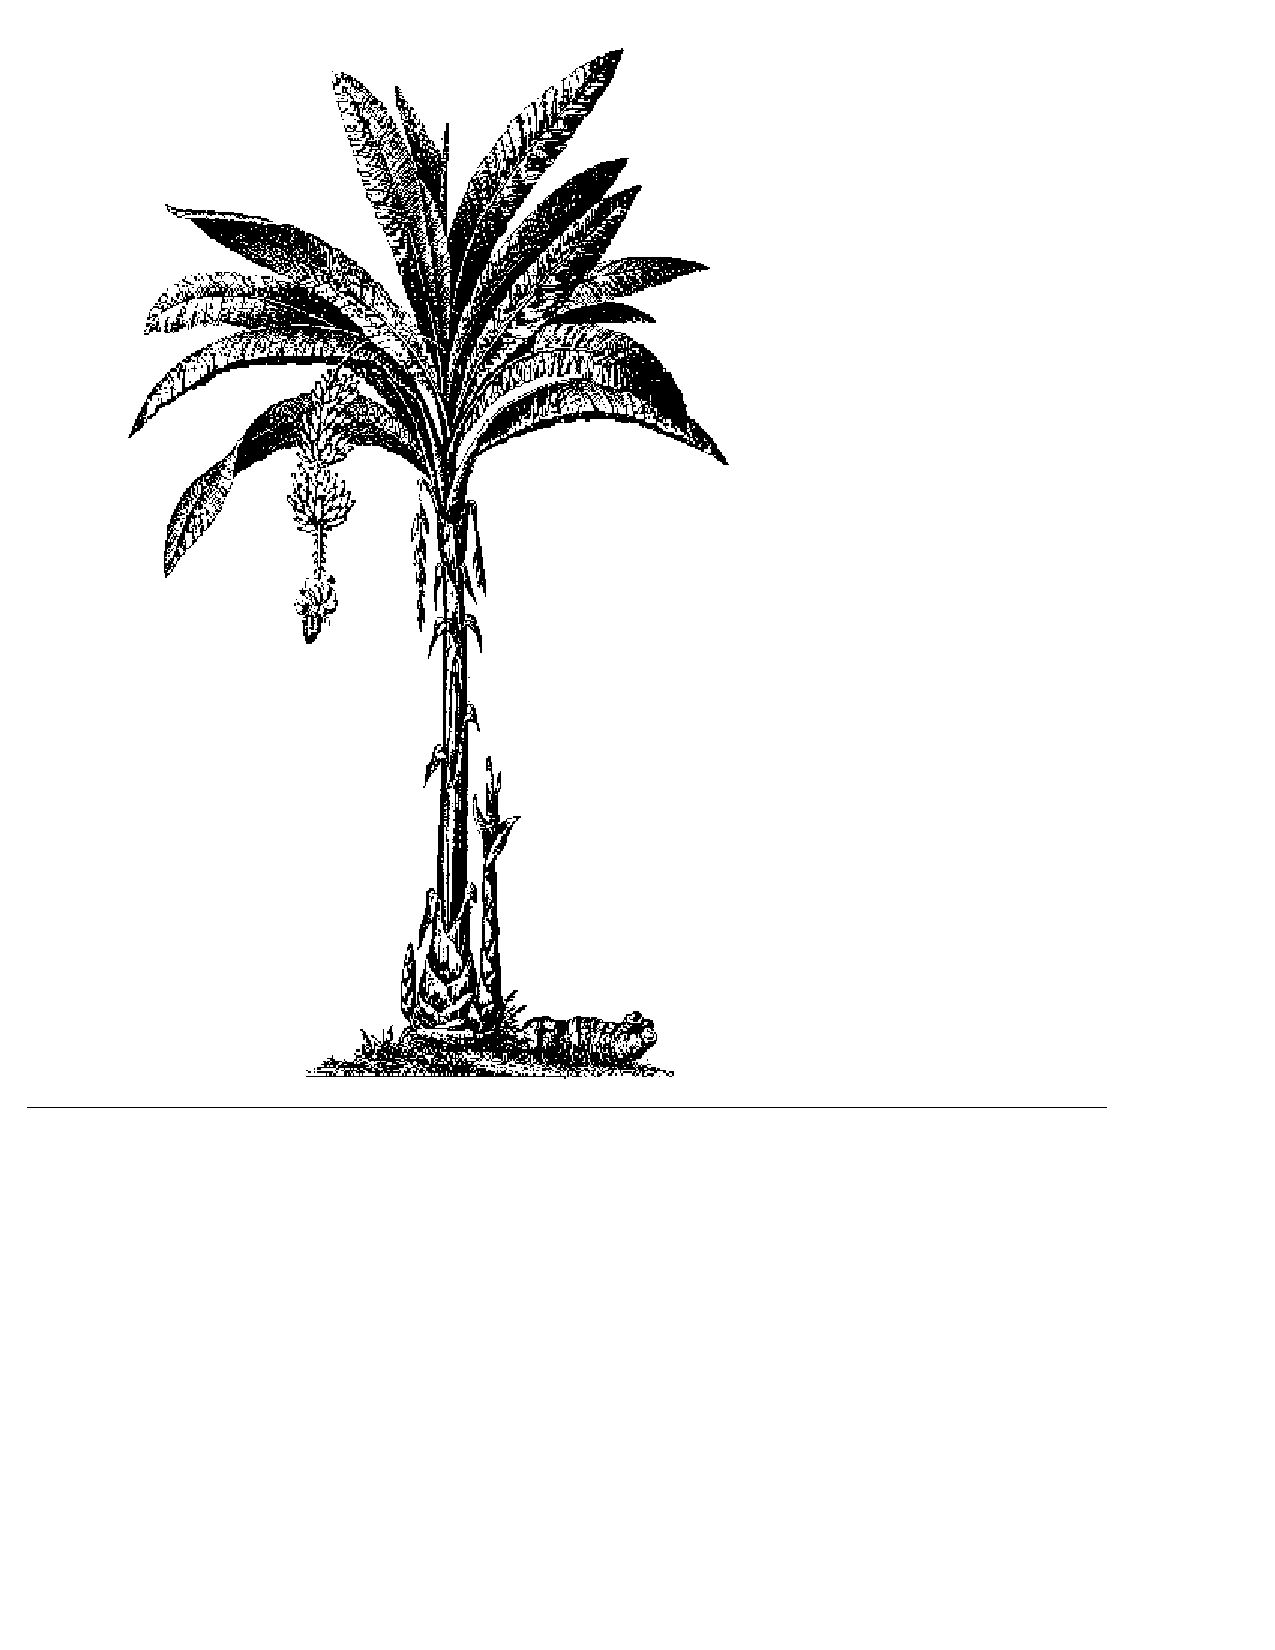
\includegraphics[scale=.1,viewport=135 624 360 700]{palm}\vspace{.5in} \\ 
%    \rule{2in}{2pt} \\ 
%    25 Signal Hill Blvd}
%    }
%    \else
%    \savebox{\Lpalme}{\parbox[t]{2in}%
%    {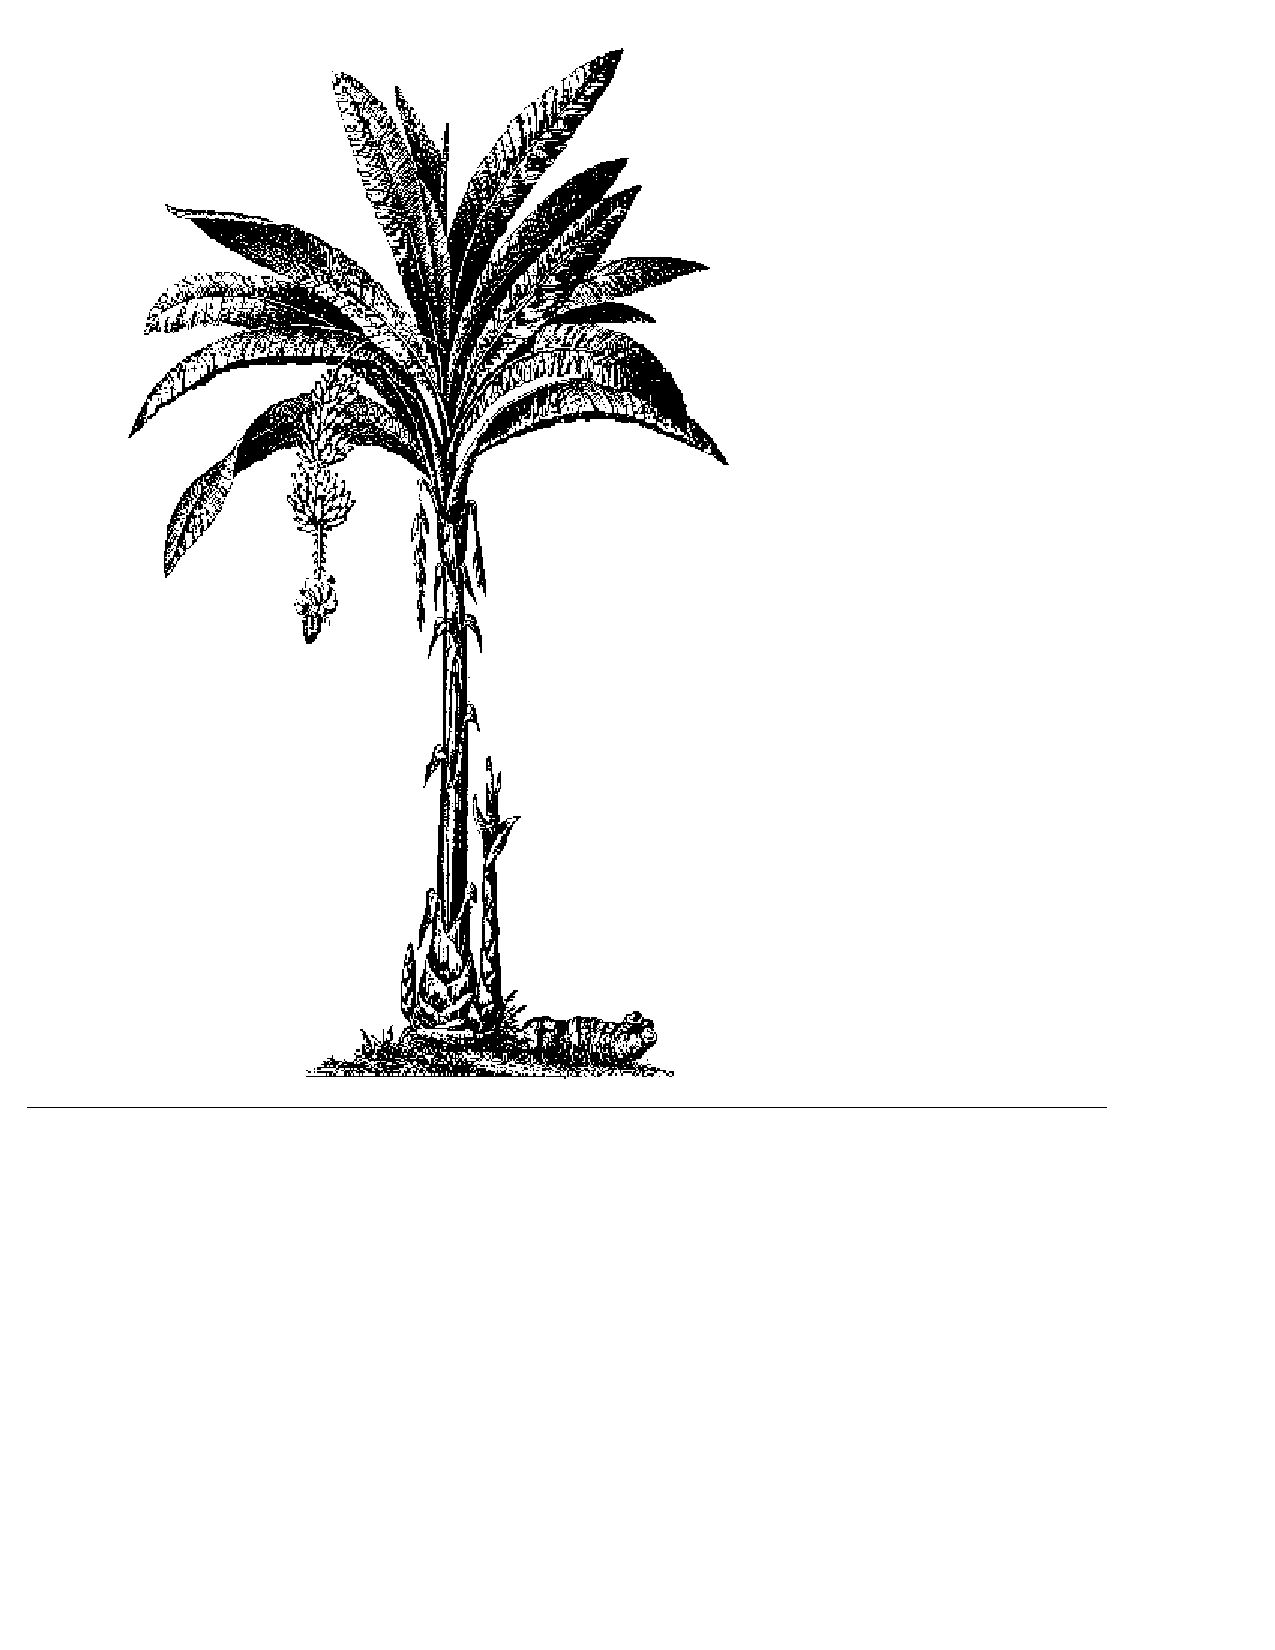
\includegraphics[scale=.1]{palm} \\ 
%    \rule{2in}{2pt} \\ 
%    25 Signal Hill Blvd}
%    }
%    \fi
%    \end{verbatim}
%    Note that the |\ifpdf| construction includes the entire |\savebox|
%    specification.  Although this is not the only manner in which this
%    system will work, it is a reliable method.  Problems can be found,
%    which are very hard to diagnose, when the |\ifpdf-\fi| construction is
%    used to control processing of portions of a specification.
%
%    \subsection{Usage tips}
%    As with any complex program, there are certain tips which can enhance 
%    the use of the program.  Here are several.  If you come up with new
%    ones, please forward them to {\tt paul@wubios.wustl.edu}; complete 
%    files demonstrating useful ideas are the most helpful.
%
%    \begin{itemize}
%    \item |geometry| is no longer used for dimension setting.  Rather, all
%      dimensions are set internally.  This is done using a combination of 
%      default values, header and footer sizes and values input from the user.
%      These include primarily the page size commands |leftmarginsize|, 
%      |textwidthsize| and |rightmarginsize|. 
%    \item When size commands are used, they will be overridden by structures.  
%      Additionally, dimensional commands are applied in order.  Inconsistencies 
%      are resolved by attending to the most recent commands, and ignoring 
%      earlier inconsistent ones.
%    \end{itemize}
%
%    \newpage
%
%    \section{Command Summary}
%    \label{sec:summ}
%    \begin{verbatim}
%    \documentstyle[options]{newlfm}
%
%    \topmarginsize{.25in} \addrfrom{Paul A. Thompson} 
%    \adr{PAT}
%    \NewlfmP{leftmarginsize=1.25in} 
%
%    \begin{document}
%    \begin{newlfm}
%       text text text
%    \end{newlfm}
%    \end{document}
%    \end{verbatim}
%
%    \vspace*{-.125in}
%
%    \begin{raggedright}
%    \begin{description}
%    \item \textbf{Letter styles:} |stdletter|, |stdletternofrom|, |busletter|,
%      |busletternofrom| 
%      (\tabpagr{letteropt})
%    \item \textbf{Letter options:} |noaddrfrom|, |printallfrom|, |printallto|,
%      |dateright|, |dateleft|, |datecenter|, |sigright|,
%      |sigleft|, |sigcenter|, |addrtoemail|, |addrtophone|, |addrtofax|,
%      |addrfromemail|, |addrfromphone|, |addrfromfax| 
%      (\tabpagr{letteropt} --- can be specified
%      either in the document-header option block or in the
%      |\newlfmP| command)
%    \item \textbf{Letter date information:} |\dateset|
%    \item \textbf{Back-ground information:} |\Background|, |\background|
%    \item \textbf{Memo styles:} |stdmemo|, |fullmemo| (\tabpagr{memoopt})
%    \item \textbf{Memo options:} |memoaddrto|, |memoemailto|, |memophoneto|,
%      |memofaxto|, |memoaddrfrom|, |memoemailfrom|, |memophonefrom|,
%      |memofaxfrom|, |memopagerto|, |memopagerfrom| (\tabpagr{memoopt} --- can be specified
%      either in the letter |\documentclass| option block or in the
%      |\newlfmP| command)
%    \item {\bf{FAX styles:}} |faxheaderpage|, |faxhba|, |faxhbb| (\tabpagr{faxopt})
%    \item {\bf{FAX options:}} |faxblocka|, |faxblockb| (\tabpagr{faxopt} --- can be specified
%      either in the letter |\documentclass| option block or in the
%      |\newlfmP| command)
%    \item {{\bf Press Release Styles:}} |stdpressrelease|%
%    \item {{\bf Press Release Options:}} |dspace|,|sspace|%
%    \item {{\bf Cellophane-window envelopes:}} |cellowindow|%
%    \item {{\bf Cellophane-window options:}} |cellodown|,|celloleft|,|cellowidth|,|celloheight|
%    \item {\bf{Address item order options:}} |orderdatefromto|,
%      |orderfromdateto|, |orderfromtodate| (can be specified
%      either in the document-header option block or in the
%      |\newlfmP| command)
%    \item {\textbf{\texttt{envlab}  options:}} |useenvlab|
%    \item {\bf{To-Address commands:}} |\nameto|, |\addressto|, |\phoneto|,
%      |\phonebto|, |\phonecto|, |\phonedto|, |\faxto|, |\emailto|, |\greetto|,
%      |\setadrto{\adrXXX}|, |\setadrto{\fixadr{XXX}}| |\regarding|,
%      |\fnameto|, |\lnameto|, |\addrt|, 
%    \item {\bf{From-Address commands:}} |\namefrom|, |\name|, |\address|,
%      |\addrfrom|, |\phone|, |\phonefrom|, |\phonebfrom|, |\phonecfrom|,
%      |\phonedfrom|, |\fax|, |\faxfrom|, |\emailfrom|,
%      |\setadrfr{\adrXXX}|, |\setadrfr{\fixadr{XXX}}|, |\fnamefrom|, |\lnamefrom|, |\addrf|
%    \item {{\bf Press Release commands:}} |\byline|, |\headline|,
%      |\release|, |\shorthead|
%    \item {\bf{End of letter commands:}} |\cclist|, |\encllist|, |\initials|,
%      |\faxmssg|, |\psitem|, |\ppsitem|, |\pppsitem|, |\re|, |\subre|
%      (\tabpagr{eolc})
%    \item {\bf{Signature commands:}} |\signature|, |\signame|, |\siglist|, |\sigacross|,
%      |\closeline|, |\sigtr|
%      (\tabpagr{sigsc})
%    \item {\bf{Horizontal spacing and sizing commands:}} 
%      |\unprleft|, |\leftmarginskipleft|, |\leftmarginsize|,
%      |\leftmarginskipright|, |\textwidth|, |\rightmarginsize|,
%      |\unprright|, |MinLeft|, |MinRight|, |minleft|, |minright|
%      (\tabpagr{spacehor} --- can be specified
%      either in the letter itself or in the
%      |\newlfmP| command; when specified in the NewlfmP statement, they are
%      specified without the ``|\|'')
%    \item {\bf{Vertical spacing and sizing commands:}} 
%      |\unprtop|, |\topmarginskip|, |\headermarginsize|, |\headermarginskip|,
%      |\leftmargintopdist|, |\rightmargintopdist|, |\memoskipbefore|, |\memoskipafter|,
%      |\dateskipbefore|, |\dateskipafter|, |\addrfromskipbefore|,
%      |\addrfromskipafter|, |\addrtoskipbefore|, |\addrtoskipafter|,
%      |\greettoskipbefore|, |\greettoskipafter|, |\textheight|,
%      |\closeskipbefore|, |\closeskipafter|,
%      |\sigskipbefore|, |\sigsize|, |\sigskipafter|,|\sigskipcolumn|,
%      |\sigskiprow|, |\postsigskipbefore|,
%      |\postsigskipafter|, |\bottommarginskip|, |\footermarginsize|,
%      |\unprbottom|, |MinHead|, |MinFoot|, |minhead|, |minfoot|
%      (\tabpagr{spacever} --- can be specified
%      either in the letter itself or in the
%      |\newlfmP| command; when specified in the NewlfmP statement, they are
%      specified without the ``|\|'')
%    \item {\bf{Wrapper commands:}} |\makeaddress{XXX}{xxx info}| creates a
%      command |\adrXXX| containing the ``xxx info'', 
%      |\makeletterhead{XXX}{stuff}| creates a command |\lthXXX| containing
%      ``stuff'' and |\makesignature{XXX}{sigstuff}| 
%      creates a command |\sigXXX| with ``sigstuff'' (\pagex{wrapc}).
%    \item {\bf{Form letters:}}
%      |\letterbody| sets the body of a form letter, while |\doletter{zz}|
%      prints the letter, |zz| is any command to be issued before the
%      letter, which will usually be a wrapper command name.
%    \item {\bf{Letterhead commands:}}  |\Lfooter|, |\Cfooter|, |\Rfooter|,
%      |\Lheader|, |\Cheader|, |\Rheader|, |\Lmargin|, |\Rmargin|,
%      |\lfooter|, |\cfooter|, |\rfooter|, |\lheader|, |\cheader|,
%      |\rheader|, |\lmargin|, |\rmargin|, |\letrh| (\tabpagr{letterhopt})
%    \item {\bf{Blanking options:}} |blankheader|, |blankfooter|,
%      |blankrmargin|, |blanklmargin|, |Blankheader|, |Blankfooter|,
%      |Blankrmargin|, |Blanklmargin|, |blankall|, |Blankall|,
%      |Blank|                    (\tabpagr{blankopt})
%    \item Extended letters: |\restlettera{text}|,  |\restletterb{text}|,
%      |\restletterc{text}|, |\restletterd{text}|, and  |\restlettere{text}| prints
%      additional pages after the signature with additional information.  
%    \item {\textbf{Printing commands:}} |\printnameto|, |\printaddrto|,
%      |\printphoneto|, |\printphoneato|, |\printphonebto|, |\printphonecto|,
%      |\printphonedto|, |\printphoneoto|, |\printphonehto|, |\printpagerto|,
%      |\printfaxto|, |\printgreetto|, |\printemailto|, |\printemailbto|,
%      |\printemailcto|, |\printlnameto|, |\printfnameto|, |\printnamefrom|,
%      |\printaddrfrom|, |\printphonefrom|, |\printphoneafrom|,
%      |\printphonebfrom|, |\printphonecfrom|, |\printphonedfrom|,
%      |\printphoneofrom|, |\printphonehfrom|, |\printpagerfrom|,
%      |\printfaxfrom|, |\printgreetfrom|, |\printemailfrom|,
%      |\printemailbfrom|, |\printemailcfrom|, |\printlnamefrom|,
%      |\printfnamefrom| (\tabpagr{printcom})
%    \end{description}
%    \end{raggedright} 
%
%    \newpage
%
% \StopEventually
%
%    \section{Code}
%    \begin{macrocode}
%<*package>
%    \end{macrocode}
%    \subsection{Preliminaries}
%    In this part we define a few commands that are used later on.
%
%    These commands are used for printing control during debugging.
%    \begin{macrocode}
\def\ifta{0}\def\iftb{0}%
\def\txa#1{\ifthenelse{\equal{\ifta}{1}}{\typeout{#1}}{}}%
\def\txb#1{}%\ifthenelse{\iftb=1}{\typeout{#1}}{}}%
%    \end{macrocode}
%
%    A number of packages are needed by this approach to letter construction.
%    These are entered here.  These packages include the following:
%    \begin{itemize*}
%    \item |keyval|: Read in key values from a single or multiple lines 
%    \item |ifthen|: Good control over conditional logic --- this actually
%                   was included above so that the boolean constructions
%                   can be used during the class file 
%    \item |setdim|:  Sets page dimensions -- similar to |chngpage|
%    \item |fancyhdr|: Control over header and footer, and several structures
%                   at one time  
%    \item |envlab|: Prints envelopes and labels in flexible ways 
%    \item |calc|:  Better arithmatic in the program
%    \item |graphicx|: External handling of graphical \info
%    \end{itemize*}
%
%    \begin{macrocode}
\RequirePackage{keyval}%
\RequirePackage{ifthen}[1997/11/02]%
\RequirePackage{ifpdf}%
\RequirePackage{setdim}%
\RequirePackage{fancyhdr}%
\RequirePackage{eso-pic}%
\RequirePackage{setspace}%
\RequirePackage{lastpage}%
\@ifundefined{ps@@empty}{%
  \ClassError{newlfm}{Version of fancyhdr.sty is not current. \MessageBreak Please obtain%
    a recent copy of fancyhdr.sty (Version 1.99d or later) from CTAN.}  {Go to CTAN and%
    download the current version of fancyhdr.sty}}{}%
\RequirePackage{calc}[1997/11/11]%
\RequirePackage{graphicx}[1997/06/09]%
\RequirePackage{rotating}[1997/06/09]%
%    \end{macrocode}
%    \paragraph{\texttt{newlength} definitions:}  
%    Begin by defining all newlength commands here, and then additionally set the
%    lengths for all those which need initialization:
%    \begin{macrocode}
\newlength{\@addr@fr@sk@b}\setlength{\@addr@fr@sk@b}{0in}%
\newlength{\@addr@fr@sk@a}\setlength{\@addr@fr@sk@a}{0in}%
\newlength{\@addr@to@sk@b}\setlength{\@addr@to@sk@b}{0in}%
\newlength{\@addr@to@sk@a}\setlength{\@addr@to@sk@a}{0in}%
\newlength{\@blka@b}\setlength{\@blka@b}{0in}%
\newlength{\@blka@a}\setlength{\@blka@a}{0in}%
\newlength{\@blkb@b}\setlength{\@blkb@b}{0in}%
\newlength{\@blkb@a}\setlength{\@blkb@a}{0in}%
\newlength{\@blkc@b}\setlength{\@blkc@b}{0in}%
\newlength{\@blkc@a}\setlength{\@blkc@a}{0in}%
\newlength{\@caption@skip@above}\setlength{\@caption@skip@above}{0in}%
\newlength{\@caption@skip@below}\setlength{\@caption@skip@below}{0in}%
\newlength{\@cello@h}\setlength{\@cello@h}{1in}%
\newlength{\@cello@w}\setlength{\@cello@w}{3in}%
\newlength{\@cello@d}\setlength{\@cello@d}{2.5in}%
\newlength{\@cello@l}\setlength{\@cello@l}{1in}%
\newlength{\@dt@sk@b}\setlength{\@dt@sk@b}{0in}%           
\newlength{\@dt@sk@a}\setlength{\@dt@sk@a}{0in}%
\newlength{\@Dth@H@L}\setlength{\@Dth@H@L}{0in}%
\newlength{\@Dth@H@C}\setlength{\@Dth@H@C}{0in}%
\newlength{\@Dth@H@R}\setlength{\@Dth@H@R}{0in}%
\newlength{\@Dth@F@L}\setlength{\@Dth@F@L}{0in}%
\newlength{\@Dth@F@C}\setlength{\@Dth@F@C}{0in}%
\newlength{\@Dth@F@R}\setlength{\@Dth@F@R}{0in}%
\newlength{\@Dth@h@l}\setlength{\@Dth@h@l}{0in}%
\newlength{\@Dth@h@c}\setlength{\@Dth@h@c}{0in}%
\newlength{\@Dth@h@r}\setlength{\@Dth@h@r}{0in}%
\newlength{\@Dth@f@l}\setlength{\@Dth@f@l}{0in}%
\newlength{\@Dth@f@c}\setlength{\@Dth@f@c}{0in}%
\newlength{\@Dth@f@r}\setlength{\@Dth@f@r}{0in}%
\newlength{\@greet@to@sk@b}\setlength{\@greet@to@sk@b}{0in}%
\newlength{\@greet@to@sk@a}\setlength{\@greet@to@sk@a}{0in}%
\newlength{\@Hgt@Head}\setlength{\@Hgt@Head}{0in}%
\newlength{\@Hrw}\setlength{\@Hrw}{1pt}%
\newlength{\@hrw}\setlength{\@hrw}{1pt}%
\newlength{\@extr@hor}\setlength{\@extr@hor}{0pt}%
\newlength{\@Frw}\setlength{\@Frw}{1pt}%
\newlength{\@frw}\setlength{\@frw}{1pt}%
\newlength{\@Hgt@Foot}\setlength{\@Hgt@Foot}{0in}%      
\newlength{\@Hgt@head}\setlength{\@Hgt@head}{0in}%
\newlength{\@Hgt@foot}\setlength{\@Hgt@foot}{0in}%
\newlength{\@Hgt@H@L}\setlength{\@Hgt@H@L}{0in}%
\newlength{\@Hgt@H@C}\setlength{\@Hgt@H@C}{0in}%
\newlength{\@Hgt@H@R}\setlength{\@Hgt@H@R}{0in}%
\newlength{\@Hgt@F@L}\setlength{\@Hgt@F@L}{0in}%
\newlength{\@Hgt@F@C}\setlength{\@Hgt@F@C}{0in}%
\newlength{\@Hgt@F@R}\setlength{\@Hgt@F@R}{0in}%
\newlength{\@Hgt@h@l}\setlength{\@Hgt@h@l}{0in}%
\newlength{\@Hgt@h@c}\setlength{\@Hgt@h@c}{0in}%
\newlength{\@Hgt@h@r}\setlength{\@Hgt@h@r}{0in}%
\newlength{\@Hgt@f@l}\setlength{\@Hgt@f@l}{0in}%
\newlength{\@Hgt@f@c}\setlength{\@Hgt@f@c}{0in}%
\newlength{\@Hgt@f@r}\setlength{\@Hgt@f@r}{0in}%
\newlength{\@lab@bl}\setlength{\@lab@bl}{0in}%
\newlength{\@lab@pl}\setlength{\@lab@pl}{0in}%
\newlength{\@lab@pw}\setlength{\@lab@pw}{0in}%
\newlength{\@lab@bh}\setlength{\@lab@bh}{0in}%
\newlength{\@lab@bw}\setlength{\@lab@bw}{0in}%
\newlength{\@lab@th}\setlength{\@lab@th}{0in}%
\newlength{\@lab@lm}\setlength{\@lab@lm}{0in}%
\newlength{\@marg@lt}\setlength{\@marg@lt}{1in}%
\newlength{\@marg@rt}\setlength{\@marg@rt}{1in}%
\newlength{\@marg@tp}\setlength{\@marg@tp}{1in}%
\newlength{\@marg@bt}\setlength{\@marg@bt}{1in}%
\newlength{\@marg@tp@a}\setlength{\@marg@tp@a}{0in}%
\newlength{\@marg@bt@a}\setlength{\@marg@bt@a}{0in}%
\newlength{\@marg@bt@b}\setlength{\@marg@bt@b}{0in}%
\newlength{\@marg@tp@b}\setlength{\@marg@tp@b}{0in}%
\newlength{\@marg@tp@s}\setlength{\@marg@tp@s}{0in}%
\newlength{\@marg@lt@r}\setlength{\@marg@lt@r}{0in}%
\newlength{\@marg@lt@l}\setlength{\@marg@lt@l}{0in}%
\newlength{\@marg@rt@r}\setlength{\@marg@rt@r}{0in}%
\newlength{\@marg@rt@l}\setlength{\@marg@rt@l}{0in}%
\newlength{\@marg@lt@tp@d}\setlength{\@marg@lt@tp@d}{0pt}%
\newlength{\@marg@rt@tp@d}\setlength{\@marg@rt@tp@d}{0pt}%
\newlength{\@Min@Hgt@Head}\setlength{\@Min@Hgt@Head}{0in}%
\newlength{\@Min@Hgt@head}\setlength{\@Min@Hgt@head}{0in}%
\newlength{\@Min@Hgt@Foot}\setlength{\@Min@Hgt@Foot}{0in}%
\newlength{\@Min@Hgt@foot}\setlength{\@Min@Hgt@foot}{0in}%
\newlength{\@Min@Hgt@Right}\setlength{\@Min@Hgt@Right}{0in}%
\newlength{\@Min@Hgt@right}\setlength{\@Min@Hgt@right}{0in}%
\newlength{\@Min@Hgt@Left}\setlength{\@Min@Hgt@Left}{0in}%
\newlength{\@Min@Hgt@left}\setlength{\@Min@Hgt@left}{0in}%
\newlength{\@Plg}\setlength{\@Plg}{0in}%
\newlength{\@Pwd}\setlength{\@Pwd}{0in}%
\newlength{\@plg}\setlength{\@plg}{0in}%
\newlength{\@pwd}\setlength{\@pwd}{0in}%
\newlength{\@post@sig@sp@a}\setlength{\@post@sig@sp@a}{0in}%
\newlength{\@post@sig@sp@b}\setlength{\@post@sig@sp@b}{0in}%
\newlength{\@pre@memo@sp}\setlength{\@pre@memo@sp}{0in}%
\newlength{\@post@memo@sp}\setlength{\@post@memo@sp}{0in}%
\newlength{\@sig@sp}\setlength{\@sig@sp}{0in}%            
\newlength{\@text@width}\setlength{\@text@width}{0in}%
\newlength{\@sig@sk@a}\setlength{\@sig@sk@a}{5pt}%
\newlength{\@sig@sk@b}\setlength{\@sig@sk@b}{5pt}%
\newlength{\@sig@sk@c}\setlength{\@sig@sk@c}{5pt}%
\newlength{\@sig@sk@r}\setlength{\@sig@sk@r}{5pt}%
\newlength{\@cls@sk@a}\setlength{\@cls@sk@a}{1em}%
\newlength{\@cls@sk@b}\setlength{\@cls@sk@b}{1em}%
\newlength{\@text@height}\setlength{\@text@height}{0in}%
\newlength{\@unpr@tp}\setlength{\@unpr@tp}{0in}%
\newlength{\@unpr@bm}\setlength{\@unpr@bm}{0in}%
\newlength{\@unpr@rt}\setlength{\@unpr@rt}{0in}%
\newlength{\@unpr@lt}\setlength{\@unpr@lt}{0in}%
\newlength{\@util}\setlength{\@util}{0in}%
\newlength{\@utila}\setlength{\@utila}{0in}%
\newlength{\@utilb}\setlength{\@utilb}{0in}%
\newlength{\@utilc}\setlength{\@utilc}{0in}%
\newlength{\@utild}\setlength{\@utild}{0in}%
\newlength{\@utile}\setlength{\@utile}{0in}%
\newlength{\@utilf}\setlength{\@utilf}{0in}%
\newlength{\@utilg}\setlength{\@utilg}{0in}%
\newlength{\@utilh}\setlength{\@utilh}{0in}%
\newlength{\@utili}\setlength{\@utili}{0in}%
\newlength{\@utilj}\setlength{\@utilj}{0in}%
\newlength{\@utilk}\setlength{\@utilk}{0in}%
\newlength{\@utill}\setlength{\@utill}{0in}%
\newlength{\@xda}\setlength{\@xda}{0in}%
\newlength{\@xdb}\setlength{\@xdb}{0in}%
\newlength{\@xdc}\setlength{\@xdc}{0in}%
\newlength{\@xdd}\setlength{\@xdd}{0in}%
\newlength{\@xde}\setlength{\@xde}{0in}%
\newlength{\@xdf}\setlength{\@xdf}{0in}%
\newlength{\@xdg}\setlength{\@xdg}{0in}%
\newlength{\@xdh}\setlength{\@xdh}{0in}%
\newlength{\@xdi}\setlength{\@xdi}{0in}%
\txa{newlength done}%
%    \end{macrocode}
%    \paragraph{\texttt{newsavebox} definitions:}  
%    Define all newsavebox commands here:
%    \begin{macrocode}
\newsavebox{\@sig@box@a}\newsavebox{\b@addr@fr}\newsavebox{\b@addr@to}%
\newsavebox{\@x@c}\newsavebox{\@x@l}\newsavebox{\@x@r}%
\newsavebox{\fba}\newsavebox{\adrfr}\newsavebox{\adrto}%
\newsavebox{\@sig@box@b}\newsavebox{\@sig@box@c}\newsavebox{\@sig@box@d}%
\newsavebox{\@sig@box@e}\newsavebox{\@sig@box@f}\newsavebox{\@sig@box@g}%
\newsavebox{\@sig@box@h}\newsavebox{\@sig@box@i}\newsavebox{\@sig@box@j}%
\newsavebox{\@rest@ltr}\newsavebox{\@resta@ltr}\newsavebox{\@restb@ltr}%
\newsavebox{\@restc@ltr}\newsavebox{\@restd@ltr}\newsavebox{\@reste@ltr}%
\txa{newsavebox done}%
%    \end{macrocode}
%    \paragraph{\texttt{newcounter} definitions:}  
%    Define all newcounter commands here:
%    \begin{macrocode}
\newcounter{@c@pos}\newcounter{figure}\newcounter{table}%
\newcounter{@sig@tot}\newcounter{@lab@tot@row}%
\newcounter{@lab@tot@col}\newcounter{@lab@cnt@row}\newcounter{@lab@cnt@col}%
\newcount\@nlfm@addr%
\newcount\@nlfm@util%
\newcount\@nlfm@uta%
\newcount\@nlfm@utb%
\txa{newcount done}%
%    \end{macrocode}
%    \paragraph{\texttt{newboolean} definitions:}  
%    Boolean variables are defined here.  Package |ifthen| defines
%    |\newboolean|.  Booleans are a good approach for simple decision-making support.  In 
%    many cases, a default value is set after the boolean is declared.
%    \begin{macrocode}
\newboolean{@addr@fr@l}%
\newboolean{@addr@fr@p}%
\newboolean{@addr@fr@e}\setboolean{@addr@fr@e}{false}%
\newboolean{@addr@fr@f}\setboolean{@addr@fr@f}{false}%
\newboolean{@addr@fr@t}\setboolean{@addr@fr@t}{false}%
\newboolean{@addr@swtch}\setboolean{@addr@swtch}{true}%
\newboolean{@addr@to@l}%
\newboolean{@addr@to@p}%
\newboolean{@addr@to@f}\setboolean{@addr@to@f}{false}%
\newboolean{@addr@to@e}\setboolean{@addr@to@e}{false}%
\newboolean{@addr@to@t}\setboolean{@addr@to@t}{false}%
\newboolean{@b@h}\setboolean{@b@h}{false}%
\newboolean{@b@f}\setboolean{@b@f}{false}%
\newboolean{@b@r}\setboolean{@b@r}{false}%
\newboolean{@b@l}\setboolean{@b@l}{false}%
\newboolean{@B@h}\setboolean{@B@h}{false}%
\newboolean{@B@f}\setboolean{@B@f}{false}%
\newboolean{@B@r}\setboolean{@B@r}{false}%
\newboolean{@B@l}\setboolean{@B@l}{false}%
\newboolean{@bg@use}\setboolean{@bg@use}{false}%
\newboolean{@Bg@use}\setboolean{@Bg@use}{false}%
\newboolean{@cello@win}\setboolean{@cello@win}{false}%
\newboolean{@cf@use}\setboolean{@cf@use}{false}%
\newboolean{@Ch@use}\setboolean{@Ch@use}{false}%
\newboolean{@Cf@use}\setboolean{@Cf@use}{false}%
\newboolean{@COf@use}\setboolean{@COf@use}{false}%
\newboolean{@CUh@use}\setboolean{@CUh@use}{false}%
\newboolean{@ch@use}\setboolean{@ch@use}{false}%
\newboolean{@do@any}%
\newboolean{@dt@l}\setboolean{@dt@l}{true}%
\newboolean{@dt@c}\setboolean{@dt@c}{false}%
\newboolean{@dt@p}%
\newboolean{@env@open}\setboolean{@env@open}{false}%
\newboolean{@env@close}\setboolean{@env@close}{false}%
\newboolean{@fax@m@run}\setboolean{@fax@m@run}{false}%
\newboolean{@fax@hdr@pg}%
\newboolean{@fax@RA}%
\newboolean{@fax@RU}%
\newboolean{@fax@bla}\setboolean{@fax@bla}{true}%
\newboolean{@fax@blb}\setboolean{@fax@blb}{false}%
\newboolean{@fl}\setboolean{@fl}{true}%
\newboolean{@Fl}\setboolean{@Fl}{true}%
\newboolean{@greet@p}%
\newboolean{@greet@l}%
\newboolean{@hl}\setboolean{@hl}{true}%
\newboolean{@Hl}\setboolean{@Hl}{true}%
\newboolean{@in@tab}%
\newboolean{@in@makeenv}\setboolean{@in@makeenv}{false}%
\newboolean{@l@am}\setboolean{@l@am}{true}%
\newboolean{@l@en}\setboolean{@l@en}{false}%
\newboolean{@l@ge}\setboolean{@l@ge}{false}%
\newboolean{@l@fr}\setboolean{@l@fr}{false}%
\newboolean{@l@ot}\setboolean{@l@ot}{false}%
\newboolean{@l@pi}\setboolean{@l@pi}{false}%
\newboolean{@lab@t}\setboolean{@lab@t}{true}%
\newboolean{@lab@cft}\setboolean{@lab@cft}{false}%
\newboolean{@lab@rft}\setboolean{@lab@rft}{false}%
\newboolean{@Lf@use}\setboolean{@Lf@use}{false}%
\newboolean{@lf@use}\setboolean{@lf@use}{false}%
\newboolean{@Lh@use}\setboolean{@Lh@use}{false}%
\newboolean{@lh@use}\setboolean{@lh@use}{false}%
\newboolean{@LOf@use}\setboolean{@LOf@use}{false}%
\newboolean{@LUh@use}\setboolean{@LUh@use}{false}%
\newboolean{@marg@lt@fl@tp}\setboolean{@marg@lt@fl@tp}{false}%
\newboolean{@marg@rt@fl@tp}\setboolean{@marg@rt@fl@tp}{false}%
\newboolean{@marg@luse}\setboolean{@marg@luse}{false}%
\newboolean{@marg@ruse}\setboolean{@marg@ruse}{false}%
\newboolean{@marg@Luse}\setboolean{@marg@Luse}{false}%
\newboolean{@marg@Ruse}\setboolean{@marg@Ruse}{false}%
\newboolean{@memo@bl}%
\newboolean{@memo@a}%
\newboolean{@memo@b}\setboolean{@memo@b}{false}%
\newboolean{@memo@c}\setboolean{@memo@c}{false}%
\newboolean{@memo@d}\setboolean{@memo@d}{false}%
\newboolean{@memo@e}\setboolean{@memo@e}{true}%
\newboolean{@memo@f}\setboolean{@memo@f}{true}%
\newboolean{@memo@g}\setboolean{@memo@g}{true}%
\newboolean{@memo@h}\setboolean{@memo@h}{false}%
\newboolean{@memo@i}\setboolean{@memo@i}{false}%
\newboolean{@memo@j}\setboolean{@memo@j}{false}%
\newboolean{@memo@k}\setboolean{@memo@k}{false}%
\newboolean{@memo@l}\setboolean{@memo@l}{false}%
\newboolean{@memo@m}\setboolean{@memo@m}{false}%
\newboolean{@memo@n}\setboolean{@memo@n}{false}%
\newboolean{@no@cen}\setboolean{@no@cen}{false}%
\newboolean{@no@spc}\setboolean{@no@spc}{false}%
\newboolean{@rest@l}\setboolean{@rest@l}{false}%
\newboolean{@resta@l}\setboolean{@resta@l}{false}%
\newboolean{@restb@l}\setboolean{@restb@l}{false}%
\newboolean{@restc@l}\setboolean{@restc@l}{false}%
\newboolean{@restd@l}\setboolean{@restd@l}{false}%
\newboolean{@reste@l}\setboolean{@reste@l}{false}%
\newboolean{@ROf@use}\setboolean{@ROf@use}{false}%
\newboolean{@Rf@use}\setboolean{@Rf@use}{false}%
\newboolean{@rf@use}\setboolean{@rf@use}{false}%
\newboolean{@Rh@use}\setboolean{@Rh@use}{false}%
\newboolean{@RUh@use}\setboolean{@RUh@use}{false}%
\newboolean{@rh@use}\setboolean{@rh@use}{false}%
\newboolean{@ov@a}\setboolean{@ov@a}{true}%
\newboolean{@ov@t}\setboolean{@ov@t}{false}%
\newboolean{@ov@l}\setboolean{@ov@l}{false}%
\newboolean{@ov@f}\setboolean{@ov@f}{false}%
\newboolean{@ov@s}\setboolean{@ov@s}{false}%
\newboolean{@pt@regard}\setboolean{@pt@regard}{false}%
\newboolean{@s@b@s}\setboolean{@s@b@s}{false}%
\newboolean{@set@env}\setboolean{@set@env}{false}%
\newboolean{@sig@p}%
\newboolean{@sig@mp}%
\newboolean{@sig@l}\setboolean{@sig@l}{false}%
\newboolean{@sig@c}\setboolean{@sig@c}{false}%
\newboolean{@space@d}\setboolean{@space@d}{true}%
\newboolean{@space@s}\setboolean{@space@s}{false}%
\newboolean{@mult@sig}\setboolean{@mult@sig}{false}%
\newboolean{@use@sig}%
\newboolean{@use@close}%
\newboolean{@use@sig@nm}%
\newboolean{@use@all@fr}%
\newboolean{@use@all@to}%
\newboolean{@use@envlab}\setboolean{@use@envlab}{false}%
\newboolean{@use@water}\setboolean{@use@water}{false}%
\newboolean{@ztila}\newboolean{@ztilb}%
\newboolean{@pr@p}\setboolean{@pr@p}{false}%
\newboolean{@pr@by}%
\txa{newboolean done}%
%    \end{macrocode}
%
%    \subsection{newlfm commands}
%    Now begin defining new commands.
%    \paragraph{Ordering of date, from-address and to-address:}
%    These commands allow the ordering of date, to-block and from-block:
%    \begin{macrocode}
\def\@d@pos#1{\def\@intd@pos{#1}}%
\def\@t@pos#1{\def\@intt@pos{#1}}%
\def\@f@pos#1{\def\@intf@pos{#1}}%
%    \end{macrocode}
%
%    \paragraph{\texttt{keyval} processing:}  When using the |keyval|
%    approach to option specification, something similar to the next code
%    must be used.  At this point, this is not 100 \% correct, and so it
%    will be altered as soon as I can figger it out.
%    \begin{macrocode}
\def\newlfmParam{\@ifnextchar[%]%
\newlx@i{\newlx@i[]}}%
\def\newlx@i[#1]{{\setkeys{ov}{#1}}}%
\def\Dimens{\@ifnextchar[%]%
\Dimens@i{\Dimens@i[]}}%
\def\Dimens@i[#1]{{\setkeys{ov}{#1}}}%
\def\Language{\@ifnextchar[%]%
\Lang@i{\Lang@i[]}}%
\def\Lang@i[#1]{{\setkeys{ov}{#1}}}%
\def\MemoParam{\@ifnextchar[%]%
\MemoP@i{\MemoP@i[]}}%
\def\MemoP@i[#1]{{\setkeys{ov}{#1}}}%
\def\LetterParam{\@ifnextchar[%]%
\LetrP@i{\LetrP@i[]}}%
\def\LetrP@i[#1]{{\setkeys{ov}{#1}}}%
\def\FAZParam{\@ifnextchar[%]%
\FAXP@i{\FAXP@i[]}}%
\def\FAXP@i[#1]{{\setkeys{ov}{#1}}}%
\def\LetterP#1{\setkeys{ov}{#1}}%
\def\newlfmP#1{\setkeys{ov}{#1}}%
\def\LanguageP#1{\setkeys{ov}{#1}}%
\def\FAXP#1{\setkeys{ov}{#1}}%
\def\DimensP#1{\setkeys{ov}{#1}}%
\def\MemoP#1{\setkeys{ov}{#1}}%
\def\iffixt#1#2{\ifthenelse{\equal{#1}{true}}{\setboolean{#2}{true}}{}}%
\def\iffixf#1#2{\ifthenelse{\equal{#1}{true}}{\setboolean{#2}{false}}{}}%
\def\iffixq#1#2{\ifthenelse{\equal{#1}{true}}{#2}{}}%
\txa{Done with key definitions sections}%
%    \end{macrocode}
%
%    \paragraph{Language option definitions:}  
%    These options define the language for the letter.  These macros are not 
%    frequently manipulated.  Basically, the strings defined here
%    set up the printing of structural elements of a memo or letter, such as
%    the ``From'' or ``To'' strings.  
%    These terms are used at various points in printing letters and memos.
%    They are American terms; your mileage may vary.  Inclusion of other
%    terms is encouraged, especially when another language group is served.
%    \begin{macrocode}
\def\DatePhrase#1{\def\@date@phr{#1}}%
\def\PhrFAXcovp#1{\def\@fax@cover@line{#1}}%
\def\PhrFAXpgcnt#1{\def\@fax@page@count{#1}}%
\def\PhrEmail#1{\def\@email@phr{#1}}%
\def\PhrFax#1{\def\@fax@phr{#1}}%
\def\PhrPager#1{\def\@pager@phr{#1}}%
\def\PhrDocument#1{\def\@doc@phr{#1}}%
\def\PhrPhone#1{\def\@phn@phr{#1}}%
\def\PhrRe#1{\def\@re@phr{#1}}%
\def\PhrSubre#1{\def\@subre@phr{#1}}%
\def\PhrCc#1{\def\@cc@phr{#1}}%
\def\PhrPs#1{\def\@ps@phr{#1}}%
\def\PhrMessage#1{\def\@m@phr{#1}}%
\def\PhrPps#1{\def\@pps@phr{#1}}%
\def\PhrPpps#1{\def\@ppps@phr{#1}}%
\def\PhrEncl#1{\def\@encl@phr{#1}}%
\def\PhrTo#1{\def\@hnto@phr{#1}}%
\def\PhrFrom#1{\def\@hnfr@phr{#1}}%
\def\PhrRegard#1{\def\@regard@phr{#1}}%
\def\PhrContact#1{\def\@contact@phr{#1}}%
\def\PhrRelease#1{\def\@release@phr{#1}}%
\def\PhrMore#1{\def\@more@phr{#1}}%
\def\PhrPRend#1{\def\@PRend@phr{#1}}%
\def\lth{}\def\sig{}\def\adr{}%
\def\letrh#1{\def\@ltr@h{#1}\setboolean{@ov@l}{true}}%       
\define@key{ov}{letrh}{\def\@ltr@h{#1}\setboolean{@ov@l}{true}}%       
\txa{Done with phr defs}%
\def\waterpage#1{\def\@water@page{#1}\setboolean{@use@water}{true}}%
\define@key{ov}{waterpage}{\def\@water@page{#1}\setboolean{@use@water}{true}}%
\txa{Waterpage}%
\def\Background#1{\def\@Backgrnd{#1}\setboolean{@Bg@use}{true}}%
\txa{Z}%
\define@key{ov}{Background}{\def\@Backgrnd{#1}\setboolean{@Bg@use}{true}}%
\def\background#1{\setboolean{@bg@use}{true}\def\@backgrnd{#1}}%
\define@key{ov}{background}{\setboolean{@bg@use}{true}\def\@backgrnd{#1}}%
\def\@adr@t{}\def\@adr@f{}\def\@ltr@h{}\def\@sig@b{}%
\def\addrt#1{\def\@adr@t{#1}\setboolean{@ov@t}{true}}%         
\define@key{ov}{addrt}{\def\@adr@t{#1}\setboolean{@ov@t}{true}}%
\def\addrf#1{\def\@adr@f{#1}\setboolean{@ov@f}{true}}%
\define@key{ov}{addrf}{\def\@adr@f{#1}\setboolean{@ov@f}{true}}%       
\def\sigtr#1{\def\@sig@b{#1}\setboolean{@ov@s}{true}}%%       
\define@key{ov}{sigtr}{\def\@sig@b{#1}\setboolean{@ov@s}{true}}%       
\def\MinHead#1{\setlength{\@Min@Hgt@Head}{#1}}%
\define@key{ov}{MinHead}{\setlength{\@Min@Hgt@Head}{#1}}%       
\def\minhead#1{\setlength{\@Min@Hgt@head}{#1}}%
\define@key{ov}{minhead}{\setlength{\@Min@Hgt@head}{#1}}%       
\def\MinLeft#1{\setlength{\@Min@Hgt@Left}{#1}}%
\define@key{ov}{MinLeft}{\setlength{\@Min@Hgt@Left}{#1}}%       
\def\minleft#1{\setlength{\@Min@Hgt@left}{#1}}%
\define@key{ov}{minleft}{\setlength{\@Min@Hgt@left}{#1}}%       
\def\MinFoot#1{\setlength{\@Min@Hgt@Foot}{#1}}%
\define@key{ov}{MinFoot}{\setlength{\@Min@Hgt@Foot}{#1}}%       
\def\minfoot#1{\setlength{\@Min@Hgt@foot}{#1}}%
\define@key{ov}{minfoot}{\setlength{\@Min@Hgt@foot}{#1}}%       
\def\MinRight#1{\setlength{\@Min@Hgt@Right}{#1}}%
\define@key{ov}{MinRight}{\setlength{\@Min@Hgt@Right}{#1}}%       
\def\minright#1{\setlength{\@Min@Hgt@right}{#1}}%
\define@key{ov}{minright}{\setlength{\@Min@Hgt@right}{#1}}%       
\def\@def@l{american}%
\def\@am@phr{%
\DatePhrase{Date}%
\PhrFAXcovp{FAX Cover Page}%
\PhrFAXpgcnt{FAX Page Count}%
\PhrFax{FAX}%
\PhrPager{Pager}%
\PhrEmail{E-mail}%
\PhrDocument{Document}%
\PhrPhone{Telephone}%
\PhrRe{Re}%
\PhrSubre{\ensuremath{\mathrm{Re}_2}}%
\PhrCc{cc}%
\PhrPs{Ps}%
\PhrMessage{Message}%
\PhrPps{Pps}%
\PhrPpps{Ppps}%
\PhrEncl{Encl}%
\PhrPager{Page}%
\PhrTo{To}%
\PhrFrom{From}%
\PhrRegard{Regarding}%
\PhrContact{Contact}%
\PhrRelease{For Immediate Release}%
\PhrMore{--- more ---}%
\PhrPRend{\# \# \#}%
}%
\InputIfFileExists{extracd.tex}%
{\typeout{Reading alternative macro definitions from extracd.tex}}%
{\typeout{All language information must be in newlfm.cls}}%
\DeclareOption{french}%
{\def\@def@l{french}\setboolean{@l@fr}{true} \@fr@phr}%
\define@key{ov}{french}[true]%
{\iffixq{#1}{\def\@def@l{french}\setboolean{@l@fr}{true} \@fr@phr}}%
\DeclareOption{german}{\def\@def@l{german}\setboolean{@l@ge}{true} \@gr@phr}%
\define@key{ov}{german}[true]%
{\iffixq{#1}{\def\@def@l{german}\setboolean{@l@ge}{true} \@gr@phr}}%
\DeclareOption{american}%
{\def\@def@l{american}\setboolean{@l@am}{true} \@am@phr}%
\define@key{ov}{american}[true]%
{\iffixq{#1}{\def\@def@l{american}\setboolean{@l@am}{true} \@am@phr}}%
\DeclareOption{english}%
{\def\@def@l{english}\setboolean{@l@en}{true} \@en@phr}%
\define@key{ov}{english}[true]%
{\iffixq{#1}{\def\@def@l{english}\setboolean{@l@en}{true} \@en@phr}}%
\DeclareOption{othlang}%
{\renewco@lgnd{\@def@l}{othlang}\setboolean{@l@ot}{true} \@ot@phr}%
\define@key{ov}{othlang}[true]%
{\iffixq{#1}{\def\@def@l{othlang}\setboolean{@l@ot}{true} \@ot@phr}}%
\DeclareOption{piglatin}%
{\def\@def@l{piglatin}\setboolean{@l@pi}{true} \@pl@phr}%
\define@key{ov}{piglatin}[true]%
{\iffixq{#1}{\def\@def@l{piglatin}\setboolean{@l@pi}{true} \@pl@phr}}%
%    \end{macrocode}
%
% \begin{macro}{Lengths}
%    Length definitions are set up here.  This is done by setting options mostly.
%    These commands are either internal (begin with |@|) or user-optional (do
%    not begin with |@|).  User-optional commands are defined in the text
%    above. 
%    \begin{macrocode}
\define@key{ov}{textwidthsize}{\setlength{\@text@width}{#1}}%
\def\textwidthsize#1{\setlength{\@text@width}{#1}}%
\define@key{ov}{textheightsize}{\setlength{\@text@height}{#1}}%
\def\textheightsize#1{\setlength{\@text@height}{#1}}%
\define@key{ov}{bottommarginskip}{\setlength{\@marg@bt@a}{#1}}%
\def\bottommarginskip#1{\setlength{\@marg@bt@a}{#1}}%
\define@key{ov}{bottommarginskipbelow}{\setlength{\@marg@bt@b}{#1}}%
\def\bottommarginskipbelow#1{\setlength{\@marg@bt@b}{#1}}%
\def\topmarginskip#1{\setlength{\@marg@tp@a}{#1}}%
\define@key{ov}{topmarginskip}{\setlength{\@marg@tp@a}{#1}}%
\def\topmarginsize#1{\setlength{\@marg@tp@s}{#1}}%
\define@key{ov}{topmarginsize}{\setlength{\@marg@tp@s}{#1}}%
\def\headermarginskip#1{\setlength{\@marg@tp@b}{#1}}%
\define@key{ov}{headermarginskip}{\setlength{\@marg@tp@b}{#1}}%
\def\rightmarginsize#1{\setlength{\@marg@rt}{#1}}%
\define@key{ov}{rightmarginsize}{\setlength{\@marg@rt}{#1}}%
\def\leftmarginsize#1{\setlength{\@marg@lt}{#1}}%
\define@key{ov}{leftmarginsize}{\setlength{\@marg@lt}{#1}}%
\def\headermarginsize#1{\setlength{\@marg@tp}{#1}}%
\define@key{ov}{headermarginsize}{\setlength{\@marg@tp}{#1}}%
\def\footermarginsize#1{\setlength{\@marg@bt}{#1}}%
\define@key{ov}{footermarginsize}{\setlength{\@marg@bt}{#1}}%
\def\leftmargintopdist#1%
{\setlength{\@marg@lt@tp@d}{#1}\setboolean{@marg@lt@fl@tp}{true}}%
\define@key{ov}{leftmargintopdist}%
{\setlength{\@marg@lt@tp@d}{#1}\setboolean{@marg@lt@fl@tp}{true}}%
\def\rightmargintopdist#1%
{\setlength{\@marg@rt@tp@d}{#1}\setboolean{@marg@rt@fl@tp}{true}}%
\define@key{ov}{rightmargintopdist}%
{\setlength{\@marg@rt@tp@d}{#1}\setboolean{@marg@rt@fl@tp}{true}}%
\define@key{ov}{leftmarginskipleft}%
{\setlength{\@marg@lt@l}{#1}\setboolean{@marg@lt@fl@tp}{false}}%
\def\leftmarginskipleft#1{\setlength{\@marg@lt@l}{#1}}%           
\define@key{ov}{rightmarginskipleft}%
{\setlength{\@marg@rt@l}{#1}\setboolean{@marg@lt@fl@tp}{false}}%
\def\rightmarginskipleft#1{\setlength{\@marg@rt@l}{#1}}%           
\def\leftmarginskipright#1{\setlength{\@marg@lt@r}{#1}}%     
\define@key{ov}{leftmarginskipright}{\setlength{\@marg@lt@r}{#1}}%     
\def\rightmarginskipright#1{\setlength{\@marg@rt@r}{#1}}%     
\define@key{ov}{rightmarginskipright}{\setlength{\@marg@rt@r}{#1}}%     
\def\dateskipbefore#1{\setlength{\@dt@sk@b}{#1}}% 
\define@key{ov}{dateskipbefore}{\setlength{\@dt@sk@b}{#1}}% 
\def\dateskipafter#1{\setlength{\@dt@sk@a}{#1}}% 
\define@key{ov}{dateskipafter}{\setlength{\@dt@sk@a}{#1}}% 
\def\addrfromskipafter#1{\setlength{\@addr@fr@sk@a}{#1}}%
\define@key{ov}{addrfromskipafter}{\setlength{\@addr@fr@sk@a}{#1}}%
\def\addrfromskipbefore#1{\setlength{\@addr@fr@sk@b}{#1}}%
\define@key{ov}{addrfromskipbefore}{\setlength{\@addr@fr@sk@b}{#1}}%
\def\addrtoskipafter#1{\setlength{\@addr@to@sk@a}{#1}}%
\define@key{ov}{addrtoskipafter}{\setlength{\@addr@to@sk@a}{#1}}%
\def\addrtoskipbefore#1{\setlength{\@addr@to@sk@b}{#1}}%
\define@key{ov}{addrtoskipbefore}{\setlength{\@addr@to@sk@b}{#1}}%
\def\greettoskipafter#1{\setlength{\@greet@to@sk@a}{#1}}% 
\define@key{ov}{greettoskipafter}{\setlength{\@greet@to@sk@a}{#1}}% 
\def\sigskipbefore#1{\setlength{\@sig@sk@b}{#1}}%
\define@key{ov}{sigskipbefore}{\setlength{\@sig@sk@b}{#1}}%
\def\sigskipafter#1{\setlength{\@sig@sk@a}{#1}}%
\define@key{ov}{sigskipafter}{\setlength{\@sig@sk@a}{#1}}%
\def\closeskipbefore#1{\setlength{\@cls@sk@b}{#1}}%
\define@key{ov}{closeskipbefore}{\setlength{\@cls@sk@b}{#1}}%
\def\closeskipafter#1{\setlength{\@cls@sk@a}{#1}}%
\define@key{ov}{closeskipafter}{\setlength{\@cls@sk@a}{#1}}%
\def\sigskipcolumn#1{\setlength{\@sig@sk@c}{#1}}%
\define@key{ov}{sigskipcolumn}{\setlength{\@sig@sk@c}{#1}}%
\def\sigskiprow#1{\setlength{\@sig@sk@r}{#1}}%
\define@key{ov}{sigskiprow}{\setlength{\@sig@sk@r}{#1}}%
\def\sigsize#1{\setlength{\@sig@sp}{#1}}%
\define@key{ov}{sigsize}{\setlength{\@sig@sp}{#1}}%
\def\postsigskipafter#1{\setlength{\@post@sig@sp@a}{#1}}% 
\define@key{ov}{postsigskipafter}{\setlength{\@post@sig@sp@a}{#1}}% %
\def\postsigskipbefore#1{\setlength{\@post@sig@sp@b}{#1}}% 
\define@key{ov}{postsigskipbefore}{\setlength{\@post@sig@sp@b}{#1}}% %
\def\memoskipafter#1{\setlength{\@post@memo@sp}{#1}}%
\define@key{ov}{memoskipafter}{\setlength{\@post@memo@sp}{#1}}%
\def\memoskipbefore#1{\setlength{\@pre@memo@sp}{#1}}%
\define@key{ov}{memoskipbefore}{\setlength{\@pre@memo@sp}{#1}}%
\def\restletter#1{\setboolean{@resta@l}{true}%
\begin{lrbox}{\@resta@ltr}\begin{minipage}{\textwidth}#1\end{minipage}\end{lrbox}}%
\def\restlettera#1{\setboolean{@resta@l}{true}%
\begin{lrbox}{\@resta@ltr}\begin{minipage}{\textwidth}#1\end{minipage}\end{lrbox}}%
\def\restletterb#1{\setboolean{@restb@l}{true}%
\begin{lrbox}{\@restb@ltr}\begin{minipage}{\textwidth}#1\end{minipage}\end{lrbox}}%
\def\restletterc#1{\setboolean{@restc@l}{true}%
\begin{lrbox}{\@restc@ltr}\begin{minipage}{\textwidth}#1\end{minipage}\end{lrbox}}%
\def\restletterd#1{\setboolean{@restd@l}{true}%
\begin{lrbox}{\@restd@ltr}\begin{minipage}{\textwidth}#1\end{minipage}\end{lrbox}}%
\def\restlettere#1{\setboolean{@reste@l}{true}%
\begin{lrbox}{\@reste@ltr}\begin{minipage}{\textwidth}#1\end{minipage}\end{lrbox}}%
\def\unprtop#1{\setlength{\@unpr@tp}{#1}}%
\define@key{ov}{unprtop}{\setlength{\@unpr@tp}{#1}}%
\def\unprbottom#1{\setlength{\@unpr@bm}{#1}}%
\define@key{ov}{unprbottom}{\setlength{\@unpr@bm}{#1}}%
\def\unprright#1{\setlength{\@unpr@rt}{#1}}%
\define@key{ov}{unprright}{\setlength{\@unpr@rt}{#1}}%
\def\unprleft#1{\setlength{\@unpr@lt}{#1}}%
\define@key{ov}{unprleft}{\setlength{\@unpr@lt}{#1}}%
%    \end{macrocode}
% \end{macro}
%
% \begin{macro}{Memos}
%    Memo definitions are set up here.  This is done by setting options
%    (for the options block in the |\documentclass| statement) or by
%    entering them into the |MemoParam| statement.
%    In the current approach to |newlfm|, both keyval and class option
%    approaches are maintained for all commands. This requires that all
%    options be processed both using |DeclareOption| and |define@key|
%    approaches.  This, at this point, does require simply duplication of
%    the code required to be processed.
%
%    \begin{macrocode}
\def\@opt@stm{%
\setboolean{@addr@fr@p}{false}%
\setboolean{@addr@to@p}{false}%
\setboolean{@memo@bl}{true}%
\setboolean{@greet@p}{false}%
\setboolean{@dt@l}{false}%
\setboolean{@dt@c}{false}%
\setboolean{@dt@p}{false}%
\setboolean{@sig@p}{false}%
\setboolean{@sig@mp}{true}%
}%
\def\@opt@stpr{%
\setboolean{@addr@fr@p}{false}%
\setboolean{@addr@to@p}{false}%
\setboolean{@memo@bl}{true}%
\setboolean{@greet@p}{false}%
\setboolean{@dt@l}{false}%
\setboolean{@dt@c}{false}%
\setboolean{@dt@p}{false}%
\setboolean{@sig@p}{false}%
\setboolean{@sig@mp}{true}%
}%
\def\@opt@flm{%
\setboolean{@addr@fr@p}{false}%
\setboolean{@addr@to@p}{false}%
\setboolean{@memo@bl}{true}%
\setboolean{@greet@p}{false}%
\setboolean{@dt@l}{false}%
\setboolean{@dt@c}{false}%
\setboolean{@dt@p}{false}%
\setboolean{@sig@p}{false}%
\setboolean{@sig@mp}{false}%
\setboolean{@memo@b}{true}%
\setboolean{@memo@c}{true}%
\setboolean{@memo@d}{true}%
\setboolean{@memo@h}{true}%
\setboolean{@memo@i}{true}%
\setboolean{@memo@j}{true}%
\setboolean{@memo@k}{true}%
\setboolean{@memo@l}{true}%
\setboolean{@memo@m}{true}%
\setboolean{@memo@n}{true}%
}%
\DeclareOption{memoaddrto}{\setboolean{@memo@b}{true}}%
\define@key{ov}{memoaddrto}[true]{\iffixt{#1}{@memo@b}}%
\DeclareOption{memoemailto}{\setboolean{@memo@k}{true}}%     
\define@key{ov}{memoemailto}[true]{\iffixt{#1}{@memo@k}}%
\DeclareOption{memophoneto}{\setboolean{@memo@c}{true}}%     
\define@key{ov}{memophoneto}[true]{\iffixt{#1}{@memo@c}}%
\DeclareOption{memopagerto}{\setboolean{@memo@n}{true}}%     
\define@key{ov}{memopagerto}[true]{\iffixt{#1}{@memo@n}}%
\DeclareOption{memofaxto}{\setboolean{@memo@d}{true}}%       
\define@key{ov}{memofaxto}[true]{\iffixt{#1}{@memo@d}}%
\DeclareOption{memoaddrfrom}{\setboolean{@memo@h}{true}}%    
\define@key{ov}{memoaddrfrom}[true]{\iffixt{#1}{@memo@h}}%
\DeclareOption{memoemailfrom}{\setboolean{@memo@l}{true}}%   
\define@key{ov}{memoemailfrom}[true]{\iffixt{#1}{@memo@l}}%
\DeclareOption{memopagerfrom}{\setboolean{@memo@m}{true}}%   
\define@key{ov}{memopagerfrom}[true]{\iffixt{#1}{@memo@m}}%
\DeclareOption{memophonefrom}{\setboolean{@memo@i}{true}}%   
\define@key{ov}{memophonefrom}[true]{\iffixt{#1}{@memo@i}}%
\DeclareOption{memofaxfrom}{\setboolean{@memo@j}{true}}%     
\define@key{ov}{memofaxfrom}[true]{\iffixt{#1}{@memo@j}}%
\DeclareOption{memodate}{\setboolean{@dt@p}{true}}%          
\define@key{ov}{memodate}[true]{\iffixt{#1}{@dt@p}}%
\DeclareOption{memonofrom}{\setboolean{@memo@e}{true}}%   
\define@key{ov}{memonofrom}[true]{\iffixt{#1}{@memo@e}}%
\DeclareOption{memonoto}{\setboolean{@memo@g}{true}}%   
\define@key{ov}{memonoto}[true]{\iffixt{#1}{@memo@g}}%
\DeclareOption{memonore}{\setboolean{@memo@f}{true}}%   
\define@key{ov}{memonore}[true]{\iffixt{#1}{@memo@f}}%
\DeclareOption{fullmemo}{\@opt@flm}%                         
\define@key{ov}{fullmemo}[true]{\iffixq{#1}{\@opt@flm}}%
\DeclareOption{stdmemo}{\@opt@stm}%                          
\define@key{ov}{stdmemo}[true]{\iffixq{#1}{\@opt@stm}}%
%    \end{macrocode}
% \end{macro}
%
% \begin{macro}{Press Releases}
%    Press release definitions are set up here.
%    Currently, there are no options.
%
%    \begin{macrocode}
\def\@opt@pr{%
\setboolean{@addr@fr@p}{true}%
\setboolean{@addr@to@p}{false}%
\setboolean{@pr@p}{true}%
\setboolean{@greet@p}{false}%
\setboolean{@dt@l}{false}%
\setboolean{@dt@c}{false}%
\setboolean{@dt@p}{false}%
\setboolean{@sig@p}{false}%
\setboolean{@sig@mp}{false}%
}%
\DeclareOption{pressrelease}{\@opt@pr}%                         
\define@key{ov}{pressrelease}[true]{\iffixq{#1}{\@opt@pr}}%
\DeclareOption{stdpressrelease}{\@opt@pr}%                          
\define@key{ov}{stdpressrelease}[true]{\iffixq{#1}{\@opt@pr}}%
\DeclareOption{dspace}{\setboolean{@space@d}{true}\setboolean{@space@s}{false}}%
\DeclareOption{sspace}{\setboolean{@space@s}{true}\setboolean{@space@d}{false}}%
\define@key{ov}{dspace}[true]{%
\iffixq{#1}{\setboolean{@space@d}{true}\setboolean{@space@s}{false}}}%
\define@key{ov}{sspace}[true]{%
\iffixq{#1}{\setboolean{@space@s}{true}\setboolean{@space@d}{false}}}%
%    \end{macrocode}
% \end{macro}
%
% \begin{macro}{Faxes}
%    These commands define the overall structures for
%    fax pages, fax blocks and fax choices.
%    \begin{macrocode}
\DeclareOption{faxhp}{\setboolean{@fax@hdr@pg}{true}\setboolean{@fax@RA}{false}}%
\DeclareOption{faxheaderpage}{\setboolean{@fax@hdr@pg}{true}\setboolean{@fax@RA}{false}}%
\define@key{ov}{faxheaderpage}[true]%
{\iffixq{#1}{\setboolean{@fax@hdr@pg}{true}\setboolean{@fax@RA}{false}}}%
\DeclareOption{faxhba}%   Print fax header block on leader in right top-margin.
{\setboolean{@fax@RA}{true}\setboolean{@fax@hdr@pg}{false}}%
\define@key{ov}{faxhba}[true]%   Print fax header block on leader in right top-margin.
{\iffixq{#1}{\setboolean{@fax@RA}{true}\setboolean{@fax@hdr@pg}{false}}}%
\DeclareOption{faxhbb}%   Print fax header block - leader - upper right quad letter 
{\setboolean{@fax@RU}{true}\setboolean{@fax@hdr@pg}{false}}%   
\DeclareOption{faxbla}%   Print FAX block in \Rheader
{\setboolean{@fax@bla}{true}\setboolean{@fax@blb}{false}}%
\DeclareOption{faxblb}%
{\setboolean{@fax@blb}{true}\setboolean{@fax@bla}{false}}%
\DeclareOption{faxblocka}%Print FAX block in \Rheader
{\setboolean{@fax@bla}{true}\setboolean{@fax@blb}{false}}%
\define@key{ov}{faxblocka}[true]%
{\iffixq{#1}{\setboolean{@fax@bla}{true}\setboolean{@fax@blb}{false}}}%
\DeclareOption{faxblockb}%
{\setboolean{@fax@blb}{true}\setboolean{@fax@bla}{false}}%
\define@key{ov}{faxblockb}[true]%
{\iffixq{#1}{\setboolean{@fax@blb}{true}\setboolean{@fax@bla}{false}}}%
%    \end{macrocode}
% \end{macro}
%
% \begin{macro}{Letters}
%    Letter definitions.  These commands define the overall structures for
%    standard letters (with and without from-addresses).  There are commands
%    for blanking of sections (blankrightmargin, etc.).  There are commands
%    for ordering of sections.  There are commands for inclusion of various
%    types of information.
%    \begin{macrocode}
\def\@opt@slr{%
\setboolean{@addr@fr@l}{false}% 
\setboolean{@addr@fr@p}{true}% 
\setboolean{@addr@to@p}{true}% 
\setboolean{@dt@p}{true}%
\setboolean{@dt@l}{false}%
\setboolean{@dt@c}{false}%
\setboolean{@greet@p}{true}%
\setboolean{@sig@p}{true}%
\setboolean{@sig@mp}{false}%
\setboolean{@addr@to@l}{true}% 
\setboolean{@memo@bl}{false}%
\setboolean{@dt@l}{false}%
\txa{In @opt@slr}%
\setboolean{@sig@l}{false}%
\setboolean{@sig@c}{false}%
\@d@pos{1}\@t@pos{3}\@f@pos{2}\setboolean{@s@b@s}{false}}%
\DeclareOption{stdletter}{\@opt@slr}%
\define@key{ov}{stdletter}[true]{\iffixq{#1}{\@opt@slr}}%
\def\@opt@sln{\setboolean{@addr@fr@l}{false}%
\setboolean{@addr@fr@p}{false}%
\setboolean{@addr@to@p}{true}%
\setboolean{@dt@p}{true}%
\setboolean{@dt@l}{false}%
\setboolean{@dt@c}{false}%
\setboolean{@greet@p}{true}%
\setboolean{@sig@p}{true}%
\setboolean{@sig@mp}{false}%
\setboolean{@addr@to@l}{true}%
\setboolean{@memo@bl}{false}%
\setboolean{@dt@l}{false}%
\txa{In @opt@sln}%
\setboolean{@sig@l}{false}%
\setboolean{@sig@c}{false}%
\@d@pos{1}\@t@pos{3}\@f@pos{2}\setboolean{@s@b@s}{false}}%
\DeclareOption{stdletternofrom} {\@opt@sln}%
\define@key{ov}{stdletternofrom}[true]{\iffixq{#1}{\@opt@sln}}%
\def\@opt@blr{\setboolean{@addr@fr@l}{true}%
\setboolean{@addr@fr@p}{true}%
\setboolean{@memo@bl}{false}%
\setboolean{@addr@to@l}{true}%
\setboolean{@dt@l}{true}%
\setboolean{@dt@c}{false}%
\txa{In @opt@blr}%
\setboolean{@sig@l}{true}%
\setboolean{@sig@c}{false}%
\setboolean{@sig@p}{true}%
\setboolean{@sig@mp}{false}%
\@d@pos{1}\@t@pos{3}\@f@pos{2}\setboolean{@s@b@s}{false}}%
\DeclareOption{busletter} {\@opt@blr}%
\define@key{ov}{busletter}[true]{\iffixq{#1}{\@opt@blr}}%
\def\@opt@bln{\setboolean{@addr@fr@l}{true}%
\setboolean{@addr@fr@p}{false}%
\setboolean{@memo@bl}{false}%
\setboolean{@addr@to@l}{true}%
\setboolean{@dt@l}{true}%
\setboolean{@dt@c}{false}%
\txa{In @opt@bln}%
\setboolean{@sig@l}{true}%
\setboolean{@sig@p}{true}%
\setboolean{@sig@mp}{false}%
\setboolean{@sig@c}{false}%
\@d@pos{1}\@t@pos{3}\@f@pos{2}\setboolean{@s@b@s}{false}}%
\DeclareOption{busletternofrom} {\@opt@bln}%
\newboolean{@test@opt}\setboolean{@test@opt}{false}%
\define@key{ov}{busletternofrom}[true]{\iffixq{#1}{\@opt@bln}}%
\DeclareOption{addrfromleft} {\setboolean{@addr@fr@l}{true}}%
\define@key{ov}{addrfromleft}[true]{\iffixt{#1}{@addr@fr@l}}%
\DeclareOption{addrfromright}{\setboolean{@addr@fr@l}{false}}%
\define@key{ov}{addrfromright}[true]{\iffixf{#1}{@addr@fr@l}}%
\DeclareOption{addrtoleft}   {\setboolean{@addr@to@l}{true}}%
\define@key{ov}{addrtoleft}[true]{\iffixt{#1}{@addr@to@l}}%
\DeclareOption{addrtoright}  {\setboolean{@addr@to@l}{false}}%
\define@key{ov}{addrtoright}[true]{\iffixf{#1}{@addr@to@l}}%
\DeclareOption{addrtoemail}  {\setboolean{@addr@to@e}{true}}%
\define@key{ov}{addrtoemail}[true]{\iffixt{#1}{@addr@to@e}}%
\DeclareOption{addrtophone}  {\setboolean{@addr@to@t}{true}}%
\define@key{ov}{addrtophone}[true]{\iffixt{#1}{@addr@to@t}}%
\DeclareOption{addrtofax}    {\setboolean{@addr@to@f}{true}}%
\DeclareOption{addrfromemail}{\setboolean{@addr@fr@e}{true}}%
\define@key{ov}{addrfromemail}[true]{\iffixt{#1}{@addr@fr@e}}%
\DeclareOption{addrfromphone}{\setboolean{@addr@fr@t}{true}}%
\define@key{ov}{addrfromphone}[true]{\iffixt{#1}{@addr@fr@t}}%
\DeclareOption{addrfromfax}  {\setboolean{@addr@fr@f}{true}}%
\define@key{ov}{addrfromfax}[true]{\iffixt{#1}{@addr@fr@f}}%
\providecommand{\boxht}{}\providecommand{\boxwd}{}\providecommand{\btwlb}{}%
\providecommand{\topht}{}\providecommand{\lftwd}{}%
\def\labpl#1{\setlength{\@lab@pl}{#1}}%
\def\boxht#1{\setlength{\@lab@bh}{#1}}%
\def\boxwd#1{\setlength{\@lab@bw}{#1}}%
\def\topht#1{\setlength{\@lab@th}{#1}}%
\def\lftwd#1{\setlength{\@lab@lm}{#1}}%
\def\btwlb#1{\setlength{\@lab@bl}{#1}}%
\def\@labname{nolines,dateno}%
\def\Alaba{\def\@labname{Avery5160,nolines,dateno}%
  \setboolean{@set@env}{true}\setboolean{@use@envlab}{false} \def\@tab@just{rrr}\labpl{10.125in}%
  \setcounter{@lab@tot@row}{10} \setcounter{@lab@tot@col}{3} \btwlb{5pt}%
  \boxht{67pt} \boxwd{174pt} \topht{38pt} \lftwd{-77pt} \setlength{\@Hgt@Foot}{0pt}}%
\def\Alabb{\def\@labname{Avery5161,nolines,dateno}%
  \setboolean{@set@env}{true}\setboolean{@use@envlab}{false} \def\@tab@just{rr}\labpl{10.125in}%
  \setcounter{@lab@tot@row}{10} \setcounter{@lab@tot@col}{2} \btwlb{8pt}%
  \boxht{67pt} \boxwd{274pt} \topht{37pt} \lftwd{-80pt} \setlength{\@Hgt@Foot}{0pt}}%
\def\Alabc{\def\@labname{Avery5162,nolines,dateno}%
  \setboolean{@set@env}{true}\setboolean{@use@envlab}{false} \def\@tab@just{rr}\labpl{9.5in}%
  \setcounter{@lab@tot@row}{7} \setcounter{@lab@tot@col}{2} \btwlb{8pt}%
  \boxht{93pt} \boxwd{274pt} \topht{62pt} \lftwd{-80pt} \setlength{\@Hgt@Foot}{0pt}}%
\def\Alabd{\def\@labname{Avery5163,nolines,dateno}%
  \setboolean{@set@env}{true}\setboolean{@use@envlab}{false} \def\@tab@just{rr}\labpl{10.125in}%
  \setcounter{@lab@tot@row}{5} \setcounter{@lab@tot@col}{2} \btwlb{8pt}%
  \boxht{139pt} \boxwd{274pt} \topht{38pt} \lftwd{-80pt} \setlength{\@Hgt@Foot}{0pt}}%
\def\Alabe{\def\@labname{Avery5164,nolines,dateno}%
  \setboolean{@set@env}{true}\setboolean{@use@envlab}{false} \def\@tab@just{rr}\labpl{10.125in}%
  \setcounter{@lab@tot@row}{3} \setcounter{@lab@tot@col}{2} \btwlb{8pt}%
  \boxht{232pt} \boxwd{274pt} \topht{38pt} \lftwd{-80pt} \setlength{\@Hgt@Foot}{0pt}}%
\DeclareOption{Avery5160}{\Alaba}%
\DeclareOption{Avery5161}{\Alabb}%
\DeclareOption{Avery5261}{\Alabb}%
\DeclareOption{Avery5162}{\Alabc}%
\DeclareOption{Avery5163}{\Alabd}%
\DeclareOption{Avery5164}{\Alabe}%
\DeclareOption{Avery5264}{\Alabe}%
\DeclareOption{labto}{\setboolean{@lab@t}{true}}%
\DeclareOption{labrowfrto}{\setboolean{@lab@rft}{true}\setboolean{@lab@t}{false}}%
\DeclareOption{labcolfrto}{\setboolean{@lab@cft}{true}\setboolean{@lab@t}{false}}%
\def\labsize#1{\def\@lab@size{#1}}%
\define@key{ov}{Avery5160}[true]{\iffixq{#1}{\Alaba}}%
\define@key{ov}{Avery5161}[true]{\iffixq{#1}{\Alabb}}%
\define@key{ov}{Avery5261}[true]{\iffixq{#1}{\Alabb}}%
\define@key{ov}{Avery5162}[true]{\iffixq{#1}{\Alabc}}%
\define@key{ov}{Avery5163}[true]{\iffixq{#1}{\Alabd}}%
\define@key{ov}{Avery5164}[true]{\iffixq{#1}{\Alabe}}%
\define@key{ov}{Avery5264}[true]{\iffixq{#1}{\Alabe}}%
\define@key{ov}{labto}[true]{\iffixq{#1}{\setboolean{@lab@t}{true}}}%
\define@key{ov}{labrowfrto}[true]{\iffixq{#1}%
{\setboolean{@lab@rft}{true}\setboolean{@lab@t}{false}}}%
\define@key{ov}{labsize}{\def\@lab@size{#1}}
\define@key{ov}{labcolfrto}[true]{\iffixq{#1}%
{\setboolean{@lab@cft}{true}\setboolean{@lab@t}{false}}}%
\DeclareOption{setuplabel}{\setboolean{@set@env}{true}\setboolean{@use@envlab}{false}}%
\define@key{ov}{setuplabel}[true]{%
\iffixq{#1}{\setboolean{@set@env}{true}\setboolean{@use@envlab}{false}}}%
\def\@dodtf{\@d@pos{1}\@t@pos{3}\@f@pos{2}\setboolean{@s@b@s}{false}}%
\def\@dofdt{\@d@pos{2}\@t@pos{3}\@f@pos{1}\setboolean{@s@b@s}{false}}%
\def\@doftd{\@d@pos{3}\@t@pos{2}\@f@pos{1}\setboolean{@s@b@s}{false}}%
\def\@dosbs{\@d@pos{1}\@t@pos{0}\@f@pos{0}\setboolean{@s@b@s}{true}}%
\DeclareOption{orderdatefromto}{\@dodtf}%
\define@key{ov}{orderdatefromto}[true]{\iffixq{#1}{\@dodtf}}%
\DeclareOption{orderfromdateto}{\@dofdt}%
\define@key{ov}{orderfromdateto}[true]{\iffixq{#1}{\@dofdt}}%
\DeclareOption{orderfromtodate}{\@doftd}%
\define@key{ov}{orderfromtodate}[true]{\iffixq{#1}{\@doftd}}%
\DeclareOption{sidebyside}{\@dosbs}%
\define@key{ov}{sidebyside}[true]{\iffixq{#1}{\@dosbs}}%
% Set right block flush top page
\DeclareOption{margflush}{\setboolean{@marg@lt@fl@tp}{true}}%
\define@key{ov}{margflush}[true]{\iffixt{#1}{@marg@lt@fl@tp}}%
% Set the marginal gap 20p
\DeclareOption{biggap}{\setboolean{@gap@small}{false}}%
% Do not print from-address.
\DeclareOption{addrfromno}{\setboolean{@addr@fr@p}{false}}%
\DeclareOption{noaddrfr}{\setboolean{@addr@fr@p}{false}}%
\DeclareOption{noaddrfrom}{\setboolean{@addr@fr@p}{false}}%
\define@key{ov}{noaddrfrom}[true]{\iffixf{#1}{@addr@fr@p}}%
% Do not print to-address.
\DeclareOption{addrtono}{\setboolean{@addr@to@p}{false}}%
\DeclareOption{noaddrto}{\setboolean{@addr@to@p}{false}}%
\define@key{ov}{noaddrto}[true]{\iffixf{#1}{@addr@to@p}}%
% Do not print greeting
\DeclareOption{greetno}{\setboolean{@greet@p}{false}}%
\define@key{ov}{nogreet}[true]{\iffixf{#1}{@greet@p}}%
% Use cello envelope
\DeclareOption{cellowindow}{\setboolean{@cello@win}{true}}%
\define@key{ov}{cellowindow}[true]{\iffixt{#1}{@cello@win}}%
% Cello dimensions
\def\celloheight#1{\setlength{\@cello@h}{#1}}%
\def\cellowidth#1{\setlength{\@cello@w}{#1}}%
\define@key{ov}{celloheight}{\celloheight{#1}}%
\define@key{ov}{cellowidth}{\cellowidth{#1}}%
% Cello placement
\def\cellodown#1{\setlength{\@cello@d}{#1}}%
\def\celloleft#1{\setlength{\@cello@l}{#1}}%
\define@key{ov}{cellodown}{\cellodown{#1}}%
\define@key{ov}{celloleft}{\celloleft{#1}}%
% Print date right-justified
\DeclareOption{dateright}{\setboolean{@dt@l}{false}\setboolean{@dt@c}{false}}%
\define@key{ov}{dateright}[true]{\iffixq{#1}{\setboolean{@dt@l}{false}\setboolean{@dt@c}{false}}}%
\def\dateright#1{\iffixq{#1}{\setboolean{@dt@l}{false}\setboolean{@dt@c}{false}}}%
% Print date left-justified
\DeclareOption{dateleft}{\setboolean{@dt@l}{true}\setboolean{@dt@c}{false}}%
\define@key{ov}{dateleft}[true]{\iffixq{#1}{\setboolean{@dt@l}{true}\setboolean{@dt@c}{false}}}%
\def\dateleft#1{\iffixq{#1}{\setboolean{@dt@l}{true}\setboolean{@dt@c}{false}}}%
% Print date centered
\DeclareOption{datecenter}{\setboolean{@dt@l}{false}\setboolean{@dt@c}{true}}%
\define@key{ov}{datecenter}[true]{\iffixq{#1}{\setboolean{@dt@l}{false}\setboolean{@dt@c}{true}}}%
\def\datecenter#1{\iffixq{#1}{\setboolean{@dt@l}{false}\setboolean{@dt@c}{true}}}%
% Do not print date
\DeclareOption{dateno}{\setboolean{@dt@p}{false}}%
\define@key{ov}{dateno}[true]{\iffixf{#1}{@dt@p}}%
\def\dateno#1{\iffixf{#1}{@dt@p}}%
% Print date
\DeclareOption{dateyes}{\setboolean{@dt@p}{true}}%
% Print signature left-justified
\def\setsigl{\setboolean{@sig@l}{true}\setboolean{@sig@c}{false}}
\def\setsigc{\setboolean{@sig@l}{false}\setboolean{@sig@c}{true}}
\def\setsigr{\setboolean{@sig@l}{false}\setboolean{@sig@c}{false}}
\DeclareOption{signatureleft}{\txa{DO fsignl}\setsigl}%
\define@key{ov}{signatureleft}[true]{\iffixq{#1}{\txa{DK fsignl}\setsigl}}%
\def\signatureleft#1{\txa{SO fsignl}\setsigl}%
\DeclareOption{sigleft}{\txa{DO asignl}\setsigl}%
\define@key{ov}{sigleft}[true]{\iffixq{#1}{\txa{DK asignl}\setsigl}}%
\def\sigleft#1{\txa{SO asignl}\setsigl}%
% Print signature centered
\DeclareOption{signaturecenter}{\txa{DO fsignc}\setsigc}%
\define@key{ov}{signaturecenter}[true]{\iffixq{#1}{\txa{DK fsignc}\setsigc}}%
\def\signaturecenter#1{\txa{SO fsignc}\setsigc}%
\DeclareOption{sigcenter}{\txa{DO asignc}\setsigc}%
\define@key{ov}{sigcenter}[true]{\iffixq{#1}{\txa{DK asignc}\setsigc}}%
\def\sigcenter#1{\txa{SO asignc}\setsigc}%
% Print signature right-justified
\DeclareOption{signatureright}{\txa{DO fsignr}\setsigr}%
\define@key{ov}{signatureright}[true]{\iffixq{#1}{\txa{DK fsignr}\setsigr}}%
\def\signatureright#1{\txa{SO fsignr}\setsigr}%
\DeclareOption{sigright}{\txa{DO asignr}\setsigr}%
\define@key{ov}{sigright}[true]{\iffixq{#1}{\txa{DK asignr}\setsigr}}%
\def\sigright#1{\txa{SO asignr}\setsigr}%
% No signature
\DeclareOption{signatureno}{\setboolean{@sig@p}{false}}%
\define@key{ov}{signatureno}[true]{\iffixf{#1}{\setboolean{@sig@p}{false}}}%
\def\signatureno#1{\setboolean{@sig@p}{false}}% 
% Print all fr \info.
\def\@fix@all@fr{%
\setboolean{@use@all@fr}{true}\setboolean{@addr@fr@p}{true}\setboolean{@addr@fr@l}{true}%
\setboolean{@addr@fr@f}{true}\setboolean{@addr@fr@e}{true}\setboolean{@addr@fr@t}{true}}%
% Print all fr \info.
\DeclareOption{printallfrom}{\@fix@all@fr}%
\define@key{ov}{printallfrom}[true]{\iffixq{#1}{\@fix@all@fr}}%
% Print all to \info.
\def\@fix@all@to{
\setboolean{@use@all@to}{true}\setboolean{@addr@to@p}{true}\setboolean{@addr@to@l}{true}%
\setboolean{@addr@to@f}{true}\setboolean{@addr@to@e}{true}\setboolean{@addr@to@t}{true}}%
\DeclareOption{printallto}{\@fix@all@to}%
\define@key{ov}{printallto}[true]{\iffixq{#1}{\@fix@all@to}}%
% Set header components to blank
\DeclareOption{blankheader}{\setboolean{@b@h}{true}}% 
\define@key{ov}{blankheader}[true]{\iffixt{#1}{@b@h}}% 
\DeclareOption{Blankheader}{\setboolean{@B@h}{true}}% 
\define@key{ov}{Blankheader}[true]{\iffixt{#1}{@B@h}}% 
% Set footer components to blank
\DeclareOption{blankfooter}{\setboolean{@b@f}{true}}%
\define@key{ov}{blankfooter}[true]{\iffixt{#1}{@b@f}}%
\DeclareOption{Blankfooter}{\setboolean{@B@f}{true}}% 
\define@key{ov}{Blankfooter}[true]{\iffixt{#1}{@B@f}}% 
% Set left margin components to blank
\DeclareOption{blanklmargin}{\setboolean{@b@l}{true}}%
\DeclareOption{blankleftmargin}{\setboolean{@b@l}{true}}% 
\define@key{ov}{blankleftmargin}[true]{\iffixt{#1}{@b@l}}% 
\DeclareOption{Blankleftmargin}{\setboolean{@B@l}{true}}%
\define@key{ov}{Blankleftmargin}[true]{\iffixt{#1}{@B@l}}%
% Set right margin components to blank
\DeclareOption{blankrmargin}{\setboolean{@b@r}{true}}%
\DeclareOption{blankrightmargin}{\setboolean{@b@r}{true}}% 
\define@key{ov}{blankrightmargin}[true]{\iffixt{#1}{@b@r}}% 
\DeclareOption{Blankrightmargin}{\setboolean{@B@r}{true}}%
\define@key{ov}{Blankrightmargin}[true]{\iffixt{#1}{@B@r}}%
% Set all components to blank
\DeclareOption{Blankall}{\setboolean{@B@f}{true}\setboolean{@B@l}{true}%
\setboolean{@B@h}{true}\setboolean{@B@r}{true}}%
\define@key{ov}{Blankall}[true]%
{\iffixq{#1}{\setboolean{@B@f}{true}\setboolean{@B@l}{true}%
\setboolean{@B@h}{true}\setboolean{@B@r}{true}}}%
\DeclareOption{blankall}{\setboolean{@b@f}{true}\setboolean{@b@l}{true}%
\setboolean{@b@h}{true}\setboolean{@b@r}{true}}%
\define@key{ov}{blankall}[true]%
{\iffixq{#1}{\setboolean{@b@f}{true}\setboolean{@b@l}{true}%
\setboolean{@b@h}{true}\setboolean{@b@r}{true}}}%
\DeclareOption{BlankTotal}% Fixed
{\setboolean{@B@f}{true}\setboolean{@B@l}{true}\setboolean{@B@h}{true}\setboolean{@B@r}{true}%
\setboolean{@b@f}{true}\setboolean{@b@l}{true}\setboolean{@b@h}{true}\setboolean{@b@r}{true}}%
\define@key{ov}{BlankTotal}[true]%
{\iffixq{#1}{\setboolean{@B@f}{true}\setboolean{@B@l}{true}\setboolean{@B@h}{true}\setboolean{@B@r}{true}%
\setboolean{@b@f}{true}\setboolean{@b@l}{true}%
\setboolean{@b@h}{true}\setboolean{@b@r}{true}}}%
\DeclareOption{useenvlab}{\setboolean{@set@env}{false}\setboolean{@use@envlab}{true}}%
\define@key{ov}{useenvlab}[true]{%
\iffixq{#1}{\setboolean{@use@envlab}{true}\setboolean{@set@env}{false}}}%
\def\@paper@type{letterpaper}%
\def\ifta{0}
\DeclareOption{letterpaper}{\def\@paper@type{letterpaper}}%
\define@key{ov}{letterpaper}[true]{\iffixq{#1}{\def\@paper@type{letterpaper}}}%
\DeclareOption{legalpaper}{\def\@paper@type{legalpaper}}%
\define@key{ov}{legalpaper}[true]{\iffixq{#1}{\def\@paper@type{legalpaper}}}%
\DeclareOption{a4paper}{\def\@paper@type{a4paper}}%
\define@key{ov}{a4paper}[true]{\iffixq{#1}{\def\@paper@type{a4paper}}}%
\DeclareOption{a3paper}{\def\@paper@type{a3paper}}%
\define@key{ov}{a3paper}[true]{\iffixq{#1}{\def\@paper@type{a3paper}}}%
\setkeys{ov}{textwidthsize=0pt,textheightsize=0pt,bottommarginskip=5pt,%
headermarginskip=0pt,rightmarginsize=72pt,leftmarginsize=72pt,bottommarginskipbelow=5pt,%
leftmargintopdist=0pt,addrtoskipafter=18pt,unprright=0pt,labsize=\normalsize,%
leftmarginskipleft=10pt,leftmarginskipright=10pt,dateskipbefore=20pt,%
dateskipafter=36pt,addrfromskipafter=36pt,addrfromskipbefore=0pt,%
greettoskipafter=18pt,sigskipbefore=12pt,sigskipafter=12pt,sigsize=72pt,%
postsigskipafter=10pt,memoskipafter=15pt,memoskipbefore=35pt,unprtop=0pt,unprbottom=0pt,%
unprleft=0pt}%
%    \end{macrocode}%
% \end{macro}
% \subsection{Executing Options}
%    Here we execute the default options to initialize certain variables.
%    \begin{macrocode}
\ExecuteOptions{\@paper@type,stdletter,american}%
%    \end{macrocode}
%
%    The |\ProcessOptions| command causes the execution of the code for every
%    option \Lopt{foo} which is declared and for which the
%    user typed the \Lopt{foo} option in his |\documentclass| command.
%    For every option \Lopt{bar} he typed, which is not declared, the
%    option is assumed to be a global option.  All options will be
%    passed as document options to any |\usepackage| command in the
%    document preamble.
%    \begin{macrocode}
\DeclareOption*{\PassOptionsToClass{\CurrentOption}{letter}}%
\ProcessOptions%
%    \end{macrocode}
%
% \begin{macro}{showdim}
%    This is here for debugging only.
%    \begin{macrocode}
\def\showdim#1{%
\txa{ * * * }%
\txa{*****************************************************************************}%
\txa{Dimensions: #1}%
% \printinunitsof{in}\pagevalues%
\txa{\string\headheight:     \the\headheight,  \string\headsep:        \the\headsep}%
\txa{\string\paperheight:    \the\paperheight, \string\paperwidth:    \the\paperwidth}%
\txa{\string\textheight:     \the\textheight,  \string\textwidth:      \the\textwidth}
\txa{\string\@colht:         \the\@colht,      \string\@colroom:       \the\@colroom}%
\txa{\string\vsize:          \the\vsize,   \string\columnwidth: \the\columnwidth}%
\txa{\string\hsize: \the\hsize, \string\linewidth: \the\linewidth}%
\txa{\string\evensidemargin: \the\evensidemargin, \string\footskip:       \the\footskip}%
\txa{\string\oddsidemargin:  \the\oddsidemargin, \string\columnsep:      \the\columnsep}%
\txa{\string\topmargin:      \the\topmargin}%
\txa{\string\marginparpush: \the\marginparpush, \string\marginparsep: \the\marginparsep}%
\txa{*****************************************************************************}%
\txa{ * * * }%
}%
%    \end{macrocode}
% \end{macro}
%    Now that all the options have been executed we can load the
%    existing copy of letter.cls.  This will ensure that the various
%    constructions which work in letters (|\begin{letter}|, etc.) will
%    continue to work in the class.  The |newlfm.cls| class adds the 
%    environment |newlfm|, which adds a number of new commands to the 
%    |letter| class, but does not remove any |letter| class commands.
%    \begin{macrocode}
\showdim{Before LoadClass}%
\PassOptionsToClass{\@paper@type,oneside,final}{letter}%
\LoadClass{letter}%
\showdim{Before addrset}%
\RequirePackage{addrset}%
\IfFileExists{afterpage.sty}{\RequirePackage{afterpage}}{}%
\IfFileExists{envlab.sty}{\RequirePackage{envlab}}{}%
\showdim{After LoadClass}%
%    \end{macrocode}%
%    Some of the page layout parameters are defined here.  Many of the values%
%    for the page layout parameters are set in geometry below.  In setting the%
%    values here, we expect that geometry will override a large number of the%
%    values.  However, the values must be assigned {\it a prior}.%
%    \begin{macrocode}%
\setlength{\voffset}{0in}%
\setlength{\itemsep}{.2em}%
\setlength{\topsep}{.2em}%
\setlength{\partopsep}{0\p@}%
\setlength{\arraycolsep}{5\p@}%
\setlength{\tabcolsep}{6\p@}%
\setlength{\arrayrulewidth}{.4\p@}%
\setlength{\doublerulesep}{2\p@}%
\setlength{\tabbingsep}{\labelsep}%
\skip\@mpfootins = \skip\footins%
\setlength{\fboxsep}{3\p@}%
\setlength{\fboxrule}{.4\p@}%
\providecommand{\geometry}{ }%
\def\geometry#1{\typeout{Command \string\geometry{items} no longer supported.}%
\typeout{newlfm supports several dimensional commands.  Please check the manual for detail.}%
}%
\renewcommand{\theequation}{\@arabic\c@equation}%
\renewcommand{\footnoterule}{%
\kern-\p@%
\hrule \@width .4\columnwidth%
\kern .6\p@}%
\long\def\@makefntext#1{%
\noindent \hangindent 5\p@%
\hb@xt@5\p@{\hss\@makefnmark}#1}%
%    \end{macrocode}%
%
%    \begin{macro}{table,figure}
%    Standard \LaTeX\ constructions |table| and |figure|
%    are not defined in |letter|.  They are added here.
%    \begin{macrocode}
\renewcommand{\thefigure}{\@arabic\c@figure}%
\providecommand{\figurename}{}\renewcommand{\figurename}{Figure}%
\providecommand{\tablename}{} \renewcommand{\tablename}{Table}%
\newcommand{\fps@figure}{tbp}\newcommand{\ftype@figure}{1}\newcommand{\ext@figure}{lof}%
\newcommand{\fnum@figure}{\figurename~\thefigure}%
\newenvironment{figure}{\@float{figure}}{\end@float}%
\newenvironment{figure*}{\@dblfloat{figure}}{\end@dblfloat}%
\renewcommand\thetable{\@arabic\c@table}%
\newcommand{\fps@table}{tbp}\newcommand{\ftype@table}{2}%
\newcommand{\ext@table}{lot}%
\newcommand{\fnum@table}{\tablename~\thetable}%
\newenvironment{table}{\@float{table}}{\end@float}%
\newenvironment{table*}{\@dblfloat{table}}{\end@dblfloat}%
\setlength\@caption@skip@above{10\p@}\setlength\@caption@skip@below{0\p@}%
\long\def\@makecaption#1#2{%
\vskip\@caption@skip@above\sbox\@tempboxa{#1: #2}%
\ifdim \wd\@tempboxa >\hsize%
#1: #2\par%
\else\global \@minipagefalse%
\hb@xt@\hsize{\hfil\box\@tempboxa\hfil}%
\fi\vskip\@caption@skip@below}%
\newcommand{\section}[1]{{\Large {\bfseries #1}}}%
%    \end{macrocode}%
% \end{macro}%
%
% \begin{macro}{Date and time macros}
%    These functions all use various system indicators of time and date to
%    furnish a time or date value to go on faxes and letters. 
%
%    \begin{macrocode}
\def\monthname{% timestamp function
\ifcase\month%
\or January\or February\or March\or April \or May\or June%
\or July\or August\or September\or October \or November\or December%
\fi%
}%
\def\timestring{%
\begingroup%
\count0 = \time \divide\count0 by 60%
\count2 = \count0 % the hour%
\count4 = \time \multiply\count0 by 60%
\advance\count4 by -\count0% the minute%
\ifnum\count4<10 \toks1 = {0} \else \toks1 = {}\fi%
\ifnum\count2<12 \toks0 = {A.M.}%
\else \toks0 = {P.M.}\advance\count2 by -12\fi%
\ifnum\count2=0 \count2 = 12 \fi % make midnight 12%
{\number\count2:\the\toks1 \number\count4%
\thinspace \the\toks0}%
\endgroup%
}%
\def\timestamp{\number\day\space\monthname\space\number\year,\space\timestring}%
\def\datestamp{\monthname\space\number\day,\space\number\year}%
%    \end{macrocode}%
% \end{macro}%
%
% \begin{macro}{Rules}%
%    These macros set up the width of rules.  They also determine whether they are printed.%
%    \begin{macrocode}%
\def\noheadline{\setboolean{@hl}{false}}%
\define@key{ov}{noheadline}[true]{\iffixq{#1}{\setboolean{@hl}{false}}}%
\def\nofootline{\setboolean{@fl}{false}}%
\define@key{ov}{nofootline}[true]{\iffixq{#1}{\setboolean{@fl}{false}}}%
\def\nolines{\setboolean{@fl}{false}\setboolean{@hl}{false}}%
\define@key{ov}{nolines}[true]{\iffixq{#1}{\setboolean{@fl}{false}\setboolean{@hl}{false}}}%
\def\noHeadline{\setboolean{@Hl}{false}}%
\define@key{ov}{noHeadline}[true]{\iffixq{#1}{\setboolean{@Hl}{false}}}%
\def\noFootline{\setboolean{@Fl}{false}}%
\define@key{ov}{noFootline}[true]{\iffixq{#1}{\setboolean{@Fl}{false}}}%
\def\noLines{\setboolean{@Fl}{false}\setboolean{@hl}{false}}%
\define@key{ov}{noLines}[true]{\iffixq{#1}{\setboolean{@Fl}{false}\setboolean{@Hl}{false}}}%
\def\@plhl{1}\def\nopheadline{\def\@plhl{0}}%
\def\@plfl{1}\def\nopfootline{\def\@plfl{0}}%
\def\Headlinewd#1{\setlength{\@Hrw}{#1}}%
\def\headlinewd#1{\setlength{\@hrw}{#1}}%
\def\Footlinewd#1{\setlength{\@Frw}{#1}}%
\def\footlinewd#1{\setlength{\@frw}{#1}}%
\define@key{ov}{Headlinewd}{\setlength{\@Hrw}{#1}}%
\define@key{ov}{headlinewd}{\setlength{\@hrw}{#1}}%
\define@key{ov}{Footlinewd}{\setlength{\@Frw}{#1}}%
\define@key{ov}{footlinewd}{\setlength{\@frw}{#1}}%
%    \end{macrocode}%
% \end{macro}%
%
%    \subsection{{\tt fancyhdr} in {\tt newlfm}} %
%    Using fancyhdr (version 1.2v or later), the |ltrhead| and |othhead| environments %
%    are set up.  The user actually does not control the \info{} using the %
%    standard macros, but rather uses Lfooter for the left footer on the %
%    letterhead and lfooter for the left footer on remaining pages.  Thus, the %
%    \info{} is transfered around in a simple manner. %
%
% \begin{macro}{ltrhead}%
%    \begin{macrocode}%
\fancypagestyle{ltrhead}{%
\def\ifta{0}%
\txa{Before setting up letterhead}%
\showdim{Letterhead}%
\fancyhf{}%
\txa{Current stored info: \string\@ltr@h:\@ltr@h}%
\fancyfoot[L]{\@Lfooter}%
\fancyfoot[C]{\@Cfooter}%
\fancyfoot[R]{\@Rfooter}%
\fancyhead[L]{\@Lheader \vspace*{\the\@marg@tp@a}}%
\fancyhead[C]{\@Cheader \vspace*{\the\@marg@tp@a}}%
\fancyhead[R]{\@Rheader \vspace*{\the\@marg@tp@a}}%
\showdim{Letterhead}%
\def\@lodd{\relax}%
\def\@rodd{\relax}%
%   \ifempty{\@LUheader}{}{\vspace*{-.5in}\@LUheader \vspace*{.5in}}%
%  }%   % section 2 goes here if we go to plan b%
%   \ifempty{\@RUheader}{}{}%
%  }%
% \@set@em@up%
% \settoheight{\@utila}{\@Rheader}\settodepth{\@utilb}{\@Rheader}\addtolength{\@utila}{\@utilb}%
% \txa{Right: \the\@utila}%
% \settoheight{\@utila}{\@Lheader}\settodepth{\@utilb}{\@Lheader}\addtolength{\@utila}{\@utilb}%
% \txa{Left: \the\@utila}%
% \settoheight{\@utila}{\@Cheader}\settodepth{\@utilb}{\@Cheader}\addtolength{\@utila}{\@utilb}%
% \txa{Center: \the\@utila}%
\txa{After setting up letterhead}%
\def\ifta{0}%
}%
%    \end{macrocode}%
% \end{macro}%
% \begin{macro}{othhead}%
%    \begin{macrocode}%
\fancypagestyle{othhead}{%
\def\ifta{0}%
\fancyhf{}%
\fancyfoot[L]{\@lfooter}%
\fancyfoot[C]{\@cfooter}%
\fancyfoot[R]{\@rfooter}%
\fancyhead[L]{\@lheader \vspace*{\the\@marg@tp@a}}%
\fancyhead[R]{\@rheader \vspace*{\the\@marg@tp@a}}%
\fancyhead[C]{\@cheader \vspace*{\the\@marg@tp@a}}%
\def\@lodd{\relax}%
\def\@rodd{\relax}%
}%
%    \end{macrocode}
% \end{macro}%
%
% \subsection{Wrapper code}
% \begin{macro}{makelth}
%    In order to use the program more efficiently, it is possible to set up a
%    database with addresses, letterhead setups and signature setups in it.
%    Rather than address placing \info{} about each letter in the letter
%    in the letter itself, \info{} is placed in the letter database file
%    and inserted into a letter using the wrapper.
%
%    \begin{enumerate}
%    \item The file is called |letrinfo.tex|.  
%    \item The file is placed somewhere on the \TeX{} path.  
%    \item In this file, place all addresses, letterhead setups and signature
%      setups as follows:
%      \begin{enumerate}
%      \item In file |letrinfo.tex|, set up a command 
%        |\makelth|{XXX}{ stuff for the letter head} 
%      \item This makes a macro out of the stuff, with the name |\lthXXX|
%      \item Issue the command |\lthXXX| prior to the start of the environment
%      \item The letterhead structure will then be used in the letter in which
%        it is called
%      \item The following commands are generally included in a letterhead
%        environment: lfooter, cfooter, rfooter, lheader, cheader, rheader,
%        Lfooter, Cfooter, Rfooter, Lheader, Cheader, Rheader, lmargin,
%        rmargin, Lmargin, Rmargin
%      \end{enumerate}
%    \end{enumerate}
%    
%    \begin{macrocode}
%</package>
%<*setdim>
\def\ifta{0}\def\iftb{0}%
\def\txa#1{\ifthenelse{\equal{\ifta}{1}}{\typeout{#1}}{}}%
\def\settext#1#2#3#4#5{%
\txa{\string\textheight: #1}\txa{\string\textwidth: #2}%
\global\setlength{\textheight}{#1}%
\global\setlength{\textwidth}{#2}%
\global\setlength{\evensidemargin}{#3}%
\global\setlength{\oddsidemargin}{#4}%
\global\setlength{\columnsep}{#5}%
\@change@text%
}%
\def\lsettext#1#2#3#4#5{%
\txa{\string\textheight: #1}\txa{\string\textwidth: #2}%
\setlength{\textheight}{#1}%
\setlength{\textwidth}{#2}%
\setlength{\evensidemargin}{#3}%
\setlength{\oddsidemargin}{#4}%
\setlength{\columnsep}{#5}%
\@lchange@text%
}%
\def\@change@text{%
\global\setlength{\@colht}{\textheight}%
\txa{\string\@colht:\the\@colht}%
\global\setlength{\@colroom}{\textheight}%
\global\setlength{\vsize}{\textheight}%
\global\setlength{\columnwidth}{\textwidth}%
\if@twocolumn%
\advance\columnwidth-\columnsep \divide\columnwidth\tw@%
\@firstcolumntrue%
\fi%
\global\setlength{\hsize}{\columnwidth}%
\global\setlength{\linewidth}{\hsize}%
}%
\def\@lchange@text{%
\setlength{\@colht}{\textheight}%
\txa{\string\@colht:\the\@colht}%
\setlength{\@colroom}{\textheight}%
\setlength{\vsize}{\textheight}%
\setlength{\columnwidth}{\textwidth}%
\if@twocolumn%
\advance\columnwidth-\columnsep \divide\columnwidth\tw@%
\@firstcolumntrue%
\fi%
\setlength{\hsize}{\columnwidth}%
\setlength{\linewidth}{\hsize}%
}%
\def\retdims{%
\showdim{Setpage A}%
\txa{In setpage: \npind}%
\global\setlength{\@xda}{\textheight}%
\global\setlength{\@xdb}{\textwidth}%
\global\setlength{\@xdc}{\evensidemargin}%
\global\setlength{\@xdd}{\oddsidemargin}%
\global\setlength{\@xde}{\columnsep}%
\global\setlength{\@xdf}{\topmargin}%
\global\setlength{\@xdg}{\headheight}%
\global\setlength{\@xdh}{\headsep}%
\global\setlength{\@xdi}{\footskip}%
}%
\def\rstdims{%
\showdim{Setpage A}%
\txa{In setpage: \npind}%
\global\setlength{\textheight}{\@xda}%
\global\setlength{\textwidth}{\@xdb}%
\global\setlength{\evensidemargin}{\@xdc}%
\global\setlength{\oddsidemargin}{\@xdd}%
\global\setlength{\columnsep}{\@xde}%
\global\setlength{\topmargin}{\@xdf}%
\global\setlength{\headheight}{\@xdg}%
\global\setlength{\headsep}{\@xdh}%
\global\setlength{\footskip}{\@xdi}%
\@change@text%
}%
\def\setpage#1#2#3#4#5#6#7#8#9{%
\showdim{Setpage A}%
\txa{In setpage: \npind}%
\settext{#1}{#2}{#3}{#4}{#5}%
\global\setlength{\topmargin}{#6}%
\global\setlength{\headheight}{#7}%
\global\setlength{\headsep}{#8}%
\global\setlength{\footskip}{#9}%
\@change@text%
\showdim{Setpage B}%
}%
\def\lsetpage#1#2#3#4#5#6#7#8#9{%
\showdim{Setpage A}%
\txa{In setpage: \npind}%
\lsettext{#1}{#2}{#3}{#4}{#5}%
\setlength{\topmargin}{#6}%
\setlength{\headheight}{#7}%
\setlength{\headsep}{#8}%
\setlength{\footskip}{#9}%
\@lchange@text%
\showdim{Setpage B}%
}%
\def\changetext#1#2#3#4#5{%
\addtolength{\textheight}{#1}%
\addtolength{\textwidth}{#2}%
\addtolength{\evensidemargin}{#3}%
\addtolength{\oddsidemargin}{#4}%
\addtolength{\columnsep}{#5}%
\@change@text%
}%
\def\changepage#1#2#3#4#5#6#7#8#9{%
\changetext{#1}{#2}{#3}{#4}{#5}%
\addtolength{\topmargin}{#6}%
\addtolength{\headheight}{#7}%
\addtolength{\headsep}{#8}%
\addtolength{\footskip}{#9}%
\@change@text%
}%
%</setdim>
%<*addrset>
%    \end{macrocode}
%    \begin{macrocode}
\def\makeletterhead#1#2{\expandafter\newcommand\csname lth#1\endcsname{#2}}%
\def\makelth#1#2{\expandafter\newcommand\csname lth#1\endcsname{#2}}%
\def\makesignature#1#2{\expandafter\newcommand\csname sig#1\endcsname{#2}}%
\def\makesig#1#2{\expandafter\newcommand\csname sig#1\endcsname{#2}}%
\def\makeadr#1#2{\expandafter\newcommand\csname adr#1\endcsname{#2}}%
\def\makeaddress#1#2{\expandafter\newcommand\csname adr#1\endcsname{#2}}%
%    \end{macrocode}
% \end{macro}
%    \begin{macrocode}
%</addrset>
%<*package>
%    \end{macrocode}
%
% \subsection{Text placement}
% \begin{macro}{Letterhead}
%    This suite of macro inserts text into a specified place for the |fancyhdr|
%    to use.  This is then later transfered into the footer of the
%    letterhead page, right side.  The remaining macros also do this, as
%    follows. r, c, l: right, center, left.  Header: top of page.  Footer:
%    bottom of page.   Capitalized: on letterhead page.  Non-capitalized: on
%    remaining pages.   
%    
%    In placing \info{} on the letterhead page, special constructions
%    allow placement {\it under} the top margin and {\it over} the footer
%    area.  These are the macros |\LOfooter|, |\COfooter|, |\ROfooter|,
%    |\LUheader|, |\CUheader| and |\RUheader|.  In the case of  |\LOfooter|,
%    |\COfooter| and |\ROfooter|, the boxed \info{} is placed over the
%    related footer section, which includes lying over the footer line (if
%    printed).  In the case of |\LUheader|, |\CUheader| and |\RUheader|, the
%    boxed \info{} is placed under the related header section, which
%    includes lying under the header line (if printed).  When any of these
%    special purpose sections are used, text length is adjusted as needed.
%    ({\bfseries NOTE:} Although this is under development, these commands are
%    not yet functional.
%    \begin{macrocode}
\providecommand{\@Lfooter}{}%    
\providecommand{\@Cfooter}{}%
\providecommand{\@Rfooter}{}%    
\providecommand{\@lfooter}{}%
\providecommand{\@cfooter}{}%    
\providecommand{\@rfooter}{}%
\providecommand{\@LOfooter}{}%   
\providecommand{\@COfooter}{}%
\providecommand{\@ROfooter}{}%   
\providecommand{\@Lheader}{}%
\providecommand{\@Cheader}{}%    
\providecommand{\@Rheader}{}%
\providecommand{\@lheader}{}%    
\providecommand{\@cheader}{}%
\providecommand{\@rheader}{}%    
\providecommand{\@LUheader}{}%
\providecommand{\@CUheader}{}%   
\providecommand{\@RUheader}{}%
\providecommand{\@Rmarg}{}%      
\providecommand{\@Lmarg}{}%
\providecommand{\@rmarg}{}%      
\providecommand{\@lmarg}{}%
\def\Lfooter#1{\setboolean{@Lf@use}{true}\def\@Lfooter{#1}}%
\def\Cfooter#1{\setboolean{@Cf@use}{true}\def\@Cfooter{#1}}%
\def\Rfooter#1{\setboolean{@Rf@use}{true}\def\@Rfooter{#1}}%
\def\LOfooter#1{\setboolean{@LOf@use}{true}\def\@LOfooter{#1}}%
\def\COfooter#1{\setboolean{@COf@use}{true}\def\@COfooter{#1}}%
\def\ROfooter#1{\setboolean{@ROf@use}{true}\def\@ROfooter{#1}}%
\def\lfooter#1{\setboolean{@lf@use}{true}\def\@lfooter{#1}}%
\def\cfooter#1{\setboolean{@cf@use}{true}\def\@cfooter{#1}}%
\def\rfooter#1{\setboolean{@rf@use}{true}\def\@rfooter{#1}}%
\def\Lheader#1{\setboolean{@Lh@use}{true}\def\@Lheader{#1}}%
\def\Cheader#1{\setboolean{@Ch@use}{true}\def\@Cheader{#1}}%
\def\Rheader#1{\setboolean{@Rh@use}{true}\def\@Rheader{#1}}%
\def\LUheader#1{\setboolean{@LUh@use}{true}\def\@LUheader{#1}}%
\def\CUheader#1{\setboolean{@CUh@use}{true}\def\@CUheader{#1}}%
\def\RUheader#1{\setboolean{@RUh@use}{true}\def\@RUheader{#1}}%      
\def\lheader#1{\setboolean{@lh@use}{true}\def\@lheader{#1}}%
\def\cheader#1{\setboolean{@ch@use}{true}\def\@cheader{#1}}%
\def\rheader#1{\setboolean{@rh@use}{true}\def\@rheader{#1}}%
\def\Rmargin#1{\def\@Rmarg{#1}\setboolean{@marg@Ruse}{true}}%
\def\Lmargin#1{\def\@Lmarg{#1}\setboolean{@marg@Luse}{true}}%
\def\rmargin#1{\def\@rmarg{#1}\setboolean{@marg@ruse}{true}}%
\def\lmargin#1{\def\@lmarg{#1}\setboolean{@marg@luse}{true}}%
%    \end{macrocode}
% \end{macro}
%
% \subsection{Memo blocks}
% \begin{macro}{\Prnt@Chk}
%    This is a conditional printing macro.  The arguments are
%    \begin{enumerate}
%    \item true: print the remainder of this item.
%    \item true: print to the left.
%    \item true: print centered.  If 2) and 3) false, print to the right.
%    \item material to print.
%    \item material or other tokens to evaluate after the previous item is aligned.
%    \item vertical space above the item.
%    \item vertical space after the item.
%    \end{enumerate}
%    \begin{macrocode}
\newcommand{\Prnt@Chk}[7]{%
  \ifthenelse{\boolean{#1}}{\ifempty{#6}{}{%
    \vspace*{-2\parskip}\vspace*{#6}}}{}%
  \ifthenelse{\boolean{#1}}%
    {\ifthenelse{\boolean{#2}}{\begin{flushleft}{#4}\end{flushleft}}%
    {\ifthenelse{\boolean{#3}}%
      {\begin{center}{#4}\end{center}}%
      {\begin{flushright}{#4}\end{flushright}}}%
    }{}%
  \ifthenelse{\boolean{#1}}{#5}{}%
  \ifthenelse{\boolean{#1}}{\ifempty{#7}{}%
    {\vspace*{-2\parskip}\vspace*{#7}}}{}%
}%
%    \end{macrocode}
% \end{macro}
%
% \begin{macro}{\memosec}
%    \label{page:memosec}
%    This section defines the text used in printing a normal memo.  
%    This will go at the top of the text block.
%   
%    If the user intends to modify the |\memosec| code to provide their 
%    own memo, the code  in |smemosec.tex| should be modified.  Save  
%    this as file |memosec.tex|, with any desired modification.
%
%    \begin{macrocode}
\newcommand{\fixphr}[2]{\strut & \parbox[t]{\the\@utilc}{#1} #2 \\}%
\def\ifta{0}%
\def\memosec{%
\def\ifta{0}\txa{Start of memosec}%
\noindent\ignorespaces%
\settowidth{\@utila}{{\bf \@hnfr@phr:\hspace*{1.25em}}}% 
\setlength{\@utilb}{\textwidth-\@utila-.1em}%
\addtolength{\@utilb}{-5pt}%   
\settowidth{\@utilc}{\@phn@phr:\hspace*{2em}}%
\settowidth{\@utild}{\@fax@phr:\hspace*{2em}}%
\ifthenelse{\lengthtest{\@utilc<\@utild}}{\setlength{\@utilc}{\the\@utild}}{}%
\settowidth{\@utild}{\@pager@phr:\hspace*{2em}}%
\ifthenelse{\lengthtest{\@utilc<\@utild}}{\setlength{\@utilc}{\the\@utild}}{}%
\settowidth{\@utild}{\@email@phr:\hspace*{2em}}%
\ifthenelse{\lengthtest{\@utilc<\@utild}}{\setlength{\@utilc}{\the\@utild}}{}%
\txa{After length tests}%
{\vspace*{-1em}\setlength{\tabcolsep}{0pt}%
\setboolean{@memo@a}{false}%
\vspace*{\@pre@memo@sp}\noindent\par%
\begin{flushleft}%
\begin{tabular}{p{\the\@utila}l}%
\ifthenelse{\boolean{@memo@g}}%
{\setboolean{@memo@a}{true}%
\strut {\bf \@hnto@phr:} & \@name@to \strut \\%
\ifthenelse{\boolean{@memo@b}}{\strut &%
\parbox[t]{\the\@utilb}{\@addr@to\strut}\strut\\}{}%
\ifthenelse{\boolean{@memo@c}}{\fixphr{\@phn@phr:}{\@phn@to}}{}%
\ifthenelse{\boolean{@memo@d}}{\fixphr{\@fax@phr:}{\@fax@to}}{}%
\ifthenelse{\boolean{@memo@n}}{\fixphr{\@pager@phr:}{\@pager@to}}{}%
\ifthenelse{\boolean{@memo@k}}{\fixphr{\@email@phr:}{\@email@to}}{}%
}{}%
\ifthenelse{\boolean{@memo@e}}%
{\setboolean{@memo@a}{true}%
\strut {\bf \@hnfr@phr:} &{\@name@fr} \strut \\%
\ifthenelse{\boolean{@memo@h}}{\strut &%
\parbox[t]{\the\@utilb}{\@addr@fr \strut} \strut \\}{}%
\ifthenelse{\boolean{@memo@i}}{\fixphr{\@phn@phr:}{\@phn@fr}}{}%
\ifthenelse{\boolean{@memo@j}}{\fixphr{\@fax@phr:}{\@fax@fr}}{}%
\ifthenelse{\boolean{@memo@m}}{\fixphr{\@pager@phr:}{\@pager@fr}}{}%
\ifthenelse{\boolean{@memo@l}}{\fixphr{\@email@phr:}{\@email@fr}}{}%
}{}%
\ifthenelse{\boolean{@memo@f}}{\setboolean{@memo@a}{true}%
\strut {\bf \@re@phr:}   &  {\@re@line} \\%
}{}%
\ifthenelse{\boolean{@dt@p}}{\strut {\bf \@date@phr:} & \@xdate \\}{}%
\ifthenelse{\boolean{@memo@a}}{\hline}{}%
\end{tabular}%
\end{flushleft}%
}%
\vspace*{\@post@memo@sp}\noindent\par%
\txa{End of memosec}
}%
\InputIfFileExists{memosec.tex}%
{\typeout{Reading {\tt memosec.tex}}}%
{\typeout{The default definition for memosec is used.  File memosec.tex doesn't exist.}}%
%    \end{macrocode}
% \end{macro}
% \subsection{Press Release blocks}
% \begin{macro}{\pressbegin}
%    \label{page:pressbegin}
%    This section defines the text used in printing a normal press release.  
%    This will go at the top of the text block.  It also sets up
%    appropriate page headers and turns off header and footer lines.
%
%    |\nolines| seemingly should disable header and footer lines, but
%    it only takes effect via |\@set@em@up|, which is only used if
%    |@ov@a| is true.  It's not in this case.  That might be a
%    problem with the implementation of |\nolines|.  It would be good
%    if the redefinition of the line width only persisted within a
%    give lfmp environment.  It's not clear that is the case.
%
%    We want |\@more@phr| (usually ``-- more --'') to appear on the
%    bottom of every page but the last.  Because the output routine may
%    be triggered when we're already into the next page, the best way to
%    handle this is with the marking mechanism.  The left mark gets the
%    {\em last\/} such mark given, while the right mark uses the first
%    right mark on the page.  So we use the left mark to set the footer.
%
%    In principle, we might use the right mark for the short header used
%    on later pages, but the existing distinction between the first and
%    other pages already handles that.
%
%    There are a lot of hard-coded distances here; eventually they
%    should perhaps be generalized.
%
%    \begin{macrocode}
\newcommand{\pressbegin}{%maybe set dimensions, esp 1 inch margins, here
\settowidth{\@utila}{\@addr@fr}%
\def\ifta{0}%
\txa{Setup beginning of press release}%
\renewcommand{\headrulewidth}{0pt}\renewcommand{\footrulewidth}{0pt}%
\setboolean{@Hl}{false}\setlength{\@Hrw}{0pt}%
\setboolean{@hl}{false}\setlength{\@hrw}{0pt}%
\setboolean{@Fl}{false}\setlength{\@Frw}{0pt}%
\setboolean{@fl}{false}\setlength{\@frw}{0pt}%
\begin{flushleft}%
\rule{\textwidth}{1pt} \par \noindent%
\centerline{\LARGE \@pr@release \strut} \par\noindent%
\rule{\textwidth}{1pt} \par \noindent
\txa{After first block}
\setlength{\tabcolsep}{0pt}%
\begin{tabular}{l@{\hspace{1em}}l}%
\textbf{\@contact@phr:} & \@name@fr \strut \\%
& \parbox[t]{\@utila}{\@addr@fr  \strut } \strut \\ %%
\ifempty{\@phn@fr}{}{\textbf{\@phn@phr:} & \@phn@fr \strut \\}%
\ifempty{\@phnb@fr}{}{\textbf{\@phn@phr:} & \@phnb@fr \strut \\}%
\ifempty{\@phnc@fr}{}{\textbf{\@phn@phr:} & \@phnc@fr \strut \\}%
\ifempty{\@phnd@fr}{}{\textbf{\@phn@phr:} & \@phnd@fr \strut \\}%
\ifempty{\@fax@fr}{}{\textbf{\@fax@phr:} & \@fax@fr \strut \\}%    % maybe email, web site?
\textbf{Date:} & \@xdate%
\end{tabular}%
\end{flushleft}%
\txa{After endflushleft}
\rule{\textwidth}{1pt} \par \noindent
\centerline{\textbf{\Large \@pr@headline}} \par \noindent
\rule{\textwidth}{1pt} \par \noindent
\ifthenelse{\boolean{@space@d}}{\begin{doublespace}}{\begin{singlespace}}%
\ifthenelse{\boolean{@pr@by}}{\noindent \@pr@byline \\}{}
\noindent
\txa{end of pressbegin}
}%
\InputIfFileExists{prsrls.tex}%
  {\typeout{Reading press release page setup from prsrls.tex}}%
  {\typeout{Press release definitions stored in newlfm.cls}}%
%    \end{macrocode}
% \end{macro}
% \subsection{ Fax blocks}
% \begin{macro}{\faxpage}
%    \label{page:faxsec}
%    Here we define a FAX page.  This separate stand-along page includes:
%    \begin{enumerate}
%    \item the term \@fax@cover@line in Huge text, boxed
%    \item From-name
%    \item Optional from-information
%    \item To-name
%    \item Optional to-information
%    \item Re-line
%    \item Additional information specified in |\faxmssg|
%    \end{enumerate}
%    
%    \begin{macrocode}
\txa{Next part}
\newcommand*{\faxpage}{{%
\def\ifta{0}\showdim{Before setpage inside faxpage}%
\lsetpage{722pt}{6.5in}{1in}{0in}{.25in}{1in}{.75in}{.25in}{.25in}%
\showdim{After setpage}%
{\def\ifta{0}\showdim{Before fax page setup A}%
\setlength{\@utila}{\paperheight}\addtolength{\@utila}{-1in}%
\setlength{\@utilb}{\paperwidth}\addtolength{\@utilb}{-2in}%
\global\setlength{\textwidth}{\paperwidth-2in}%
\txa{\string\paperheight:\paperheight,\string\@utila:\the\@utila}%
\txa{\string\paperwidth:\paperwidth,\string\@utilb:\the\@utilb}\gdef\npind{A1}%
\@clear@box%
\def\ifta{0}% 
\txa{\string\paperheight:\the\paperheight,\string\@utila:\the\@utila}%
\txa{\string\paperwidth:\the\paperwidth,\string\@utilb:\the\@utilb}%
\txa{\string\textheight:\the\textheight,\string\textwidth:\the\textwidth}%
\newpage\c@page\@ne\interlinepenalty=200%
\showdim{Before fax page setup B}%
\thispagestyle{empty}%
\vspace*{-\the\@Hgt@Head}\vspace*{.5in}%
\showdim{Inside fax page specification}%
\begin{center}%
\framebox{\Huge{\@fax@cover@line}} \\%
\vspace*{.5in} \Large{\@fax@page@count: \ref{totpage}} \\%
\vspace*{.5in} \Large{\timestamp} \\%
\end{center}%
\settowidth{\@utila}{\LARGE{\@hnto@phr:}}%
\settowidth{\@utilb}{\LARGE{\@hnfr@phr:}}%
\ifthenelse{\lengthtest{\@utila<\@utilb}}{\setlength{\@utila}{\@utilb}}{}%
\settowidth{\@utilb}{\LARGE{\@m@phr:}}%
\ifthenelse{\lengthtest{\@utila<\@utilb}}{\setlength{\@utila}{\@utilb}}{}%
\setlength{\tabcolsep}{0pt}%
\setlength{\@utilb}{\the\textwidth-\the\@utila}%
\txa{Lengths:\the\textwidth, \the\@utila, \the\@utilb}%
\begin{tabular}{p{\the\@utila}p{\the\@utilb}} \hline \\%
\LARGE{\@hnto@phr:} & \parbox[t]{\@utilb}{\@name@to \strut \\ \@addr@to \strut%
\ifempty{\@phn@to}{}{\\ \@phn@phr:\space\@phn@to \strut}%
\ifempty{\@phnb@to}{}{\\ \@phn@phr:\space\@phnb@to \strut}%
\ifempty{\@phnc@to}{}{\\ \@phn@phr:\space\@phnc@to \strut}%
\ifempty{\@phnd@to}{}{\\ \@phn@phr:\space\@phnd@to \strut}%
\ifempty{\@fax@to}{}{\\ \@fax@phr:\space\@fax@to \strut}} \vspace*{5pt} \\ \hline \vspace*{5pt}%
\LARGE{\@hnfr@phr:} & \vspace*{5pt}%
\parbox[t]{\@utilb}{\@name@fr \strut \\ \@addr@fr \strut %%
\ifempty{\@phn@fr}{}{\\ \@phn@phr:\space\@phn@fr \strut}%
\ifempty{\@phnb@fr}{}{\\ \@phn@phr:\space\@phnb@fr \strut}%
\ifempty{\@phnc@fr}{}{\\ \@phn@phr:\space\@phnc@fr \strut}%
\ifempty{\@phnd@fr}{}{\\ \@phn@phr:\space\@phnd@fr \strut}%
\ifempty{\@fax@fr}{}{\\ \@fax@phr:\space\@fax@fr \strut}} \vspace*{5pt} \\  \hline%
\vspace*{5pt}% 
\strut \LARGE{\@re@phr:} & \strut%
\ifthenelse{\equal{\@re@line}{---BLANK---}}{}{\@re@line}\strut \\%
\ifempty{\@fax@mssg}{}{ \strut%
\LARGE{\@m@phr:} \strut &%
\parbox[t]{\@utilb}{\strut \@fax@mssg} \strut \\ \hline}%
\end{tabular}}%
\def\ifta{0}\showdim{End of fax page setup }%
\@dim@resetfalse%
\txa{After dimreset}%
\gdef\npind{F}%
\txa{Before newpage}%
\newpage%
\txa{After newpage}%
}}%
\InputIfFileExists{faxpage.tex}%
  {\typeout{Reading FAX page definitions from faxpage.tex}}%
  {\typeout{faxpage definitions stored in newlfm.cls}}%
%    \end{macrocode}
% \end{macro}
% \begin{macro}{faxblocka}
%    Here we define FAX block a.  This block is inserted in several places in
%    the letter, by chosing several letter styles.  It can also be inserted in
%    several blocks by user choice.  Fax Block A includes
%    1.) name-from, 2.) fax-from, 3.) name-to, 4.) fax-to, and 5.) re-line.
%    FAX Block A is boxed in a frame.
%    \begin{macrocode}
\newcommand{\faxblocka}{%
\sbox{\fba}{%
\framebox[3.0in]{\parbox[b]{3.0in}{\setlength{\tabcolsep}{0pt}%
\begin{tabular}{p{1.0in}p{2in}}%
\multicolumn{2}{l}{\Large \hspace*{.25in}%
\@fax@phr{} \@doc@phr} \\ \hline%
\@hnfr@phr:\space & \@name@fr \\%
\@fax@phr:\space & \@fax@fr \\ \hline%
\@hnto@phr:\space & \@name@to \\%
\@fax@phr:\space & \@fax@to \\ \hline%
\@re@phr: & \@re@line%
\end{tabular}}}}}%
%    \end{macrocode}
% \end{macro}
% \begin{macro}{faxblockb}
%    Here we define FAX block b.  This block is inserted in several places in
%    the letter, by chosing several letter styles.  It can also be inserted in
%    several blocks by user choice.  Fax Block B includes
%    1.) name-from, 2.) fax-from, 3.) phone-from, 4.) name-to, 5.) fax-to,
%    6.) phone to, and 7.) re-line.
%    FAX Block B is boxed in a frame.
%    \begin{macrocode}
\newcommand{\faxblockb}{%
{\parbox[t]{\textwidth}{\fbox{%
\begin{tabular}{llll}%
\@hnfr@phr:\space & \@name@fr & \@hnto@phr:\space & \@name@to \\%
\@fax@phr:\space & \@fax@fr & \@fax@phr:\space & \@fax@to \\%
\@phn@phr:\space & \@phn@fr & \@phn@phr:\space & \@phn@to \\%
\@re@phr: & \multicolumn{3}{l}{\parbox[t]{2in}{\@re@line}} \\%
\end{tabular}%
}}}}%
%    \end{macrocode}
% \end{macro}
% \subsection{Start of letter document}
% \begin{macro}{\openlfm}
%    Begin letter here.  First check for left margin boxes; if one has been
%    specified, set it into the margin, and change the margin spacing
%    accordingly.  After that, the left, right and center under-margin boxes
%    are checked.  If this is a memo, this \info{} is printed next.
%    Finally, we print (optionally) date, from-address, to-address and opening
%    salutation.
%    \begin{macrocode}
\newcommand{\ifempty}[3]{\ifthenelse{\equal{#1}{}}{#2}{#3}}%
\newcommand{\ifpempty}[3]{\ifthenelse{\equal{\protect#1}{}}{#2}{#3}}%
\newcommand{\@prnt@sec}[1]{%  Actual printing of addresses here
\ifthenelse{#1=\@intd@pos}%
{\Prnt@Chk{@dt@p}{@dt@l}{@dt@c}{\@xdate}{}{\@dt@sk@b}{\@dt@sk@a}}{}%
\ifthenelse{#1=\@intf@pos}%
{\Prnt@Chk{@addr@fr@p}{@addr@fr@l}{@no@cen}%
{\usebox{\b@addr@fr}}{}{\@addr@fr@sk@b}{\@addr@fr@sk@a}}{}%
\ifthenelse{#1=\@intt@pos}%
{\Prnt@Chk{@addr@to@p}{@addr@to@l}{@no@cen}%
{\usebox{\b@addr@to}}{}{\@addr@to@sk@b}{\@addr@to@sk@a}}{}%
}%
%    \end{macrocode}
%    This is the actual section for openlfm.
%    \begin{macrocode}
\newcommand*{\openlfm}{%
\def\ifta{0}%
\ifthenelse{\boolean{@use@water}}%
{\ClearShipoutPicture%
\AddToShipoutPicture{\includegraphics[natheight=11in,natwidth=8.5in]{\@water@page}}%
}{}%
\ifthenelse{\boolean{@marg@Ruse}}%             Here we set up right-side marginal notes
{\setlength{\@utile}{-\@Hgt@Head+\@marg@rt@tp@d}% Adjust column top to leftmargintopdist
\normalmarginpar%
\marginpar{\vspace*{\the\@utile} \hspace*{\@marg@rt@l}\hspace*{-\marginparsep} \@Rmarg}}{}%
\ifthenelse{\boolean{@marg@Luse}}%             Here we set up left-side marginal notes
{\setlength{\@utile}{-\@Hgt@Head+\@marg@lt@tp@d}% Adjust column top to leftmargintopdist
\reversemarginpar\txa{Left margin}%
\marginpar{\vspace*{\the\@utile} \hspace*{\@marg@lt@l} \@Lmarg}}{}%
\ifpempty{\@LUheader}{}{\@LUheader \hfill}%
\ifpempty{\@CUheader}{}{\hfill \@CUheader \hfill}%
\ifpempty{\@RUheader}{}{\hfill \@RUheader}%
\txa{Running memosec}%                         Memo processing    
\ifthenelse{\boolean{@memo@bl}}%
{{\memosec}\setboolean{@dt@p}{false}%
\setboolean{@no@spc}{true}}% %Memo
{}%
\txa{Running pressbegin}%
\ifthenelse{\boolean{@pr@p}}%
{\pressbegin%                                Press release processing
\txa{here we go again - out of pressbegin}
\setboolean{@no@spc}{true}}{}% % Press Release
\sbox{\b@addr@fr}{\noindent\setlength{\tabcolsep}{0pt}% Address-from into a box
\raggedleft\begin{tabular}{l@{}}%
\noindent\ignorespaces\@addr@fr%
\ifthenelse{\boolean{@addr@fr@t}}{\\ \@phn@phr: \@phn@fr}{}%
\ifthenelse{\boolean{@addr@fr@f}}{\\ \@fax@phr: \@fax@fr}{}%
\ifthenelse{\boolean{@addr@fr@e}}{\\ \@email@phr: \@email@fr}{}%
\end{tabular}}%
\settowidth{\@utilc}{\usebox{\b@addr@fr}}%
\sbox{\b@addr@fr}{\noindent\setlength{\tabcolsep}{0pt}%
\parbox[t]{\@utilc}{\noindent%
\begin{tabular}{l@{}}%
\ignorespaces\@addr@fr%
\ifthenelse{\boolean{@addr@fr@t}}{\\ \@phn@phr: \@phn@fr}{}%
\ifthenelse{\boolean{@addr@fr@f}}{\\ \@fax@phr: \@fax@fr}{}%
\ifthenelse{\boolean{@addr@fr@e}}{\\ \@email@phr: \@email@fr}{}%
\end{tabular}}}%
\sbox{\b@addr@to}{\noindent\setlength{\tabcolsep}{0pt}%Address-to into a box
\raggedleft\begin{tabular}{l@{}}%
\noindent\ignorespaces\@name@to \strut \\ \@addr@to%
\ifthenelse{\boolean{@addr@to@t}}{\\ \@phn@phr: \@phn@to}{}%
\ifthenelse{\boolean{@addr@to@f}}{\\ \@fax@phr: \@fax@to}{}%
\ifthenelse{\boolean{@addr@to@e}}{\\ \@email@phr: \@email@to}{}%
\end{tabular}}%
\settowidth{\@utild}{\usebox{\b@addr@to}}%
\sbox{\b@addr@to}{\noindent\setlength{\tabcolsep}{0pt}%
\parbox[t]{\@utild}{\noindent%
\begin{tabular}{l@{}}%
\ignorespaces\@name@to \strut \\ \@addr@to%
\ifthenelse{\boolean{@addr@to@t}}{\\ \@phn@phr: \@phn@to}{}%
\ifthenelse{\boolean{@addr@to@f}}{\\ \@fax@phr: \@fax@to}{}%
\ifthenelse{\boolean{@addr@to@e}}{\\ \@email@phr: \@email@to}{}%
\end{tabular}}}%
\ifthenelse{\boolean{@no@spc}}{}{%
\ifthenelse{\boolean{@s@b@s}}{\par\noindent{\usebox{\b@addr@to} \hfill \usebox{\b@addr@fr}}}{}%
\setcounter{@c@pos}{1} \@prnt@sec{\the@c@pos}%  Print from and to addresses and date
\setcounter{@c@pos}{2} \@prnt@sec{\the@c@pos}%
\setcounter{@c@pos}{3} \@prnt@sec{\the@c@pos}%
\setboolean{@greet@l}{true}%
\ifthenelse{\boolean{@pt@regard}}{\@regard@phr: \@regard@line}{}%
\Prnt@Chk{@greet@p}{@greet@l}{@no@cen}%
{\par\@greet@to\par\nobreak}{}{}{\@greet@to@sk@a}%
}%
\txa{End of openlfm}%
}%
%    \end{macrocode}
% \end{macro}
% \subsection{Close of document section}
% \begin{macro}{closlfm}
%    In this section, the letter is terminated.  Several things happen here:
%    \begin{enumerate}
%    \item If signature block is to be printed, it is printed
%    \item If signature itself is to be printed, it is printed; otherwise,
%      just skip a reasonable amount of vertical space, to allow document to
%      be signed 
%    \item If sender name is to be printed, it is printed
%    \item For press releases, output |\PhrPRend| and blank the
%      ---more--- in the footer.  The marking mechanism is the proper
%      way to do this, avoiding the unlikely case where we might blank the footer
%      and then have the previous page output.
%    \end{enumerate}
%    \begin{macrocode}
\def\ifta{0}
\def\@fix@one@box{%
\settowidth{\@utila}{\setlength{\tabcolsep}{0pt}%
\begin{tabular}{l}%
\hspace*{1pt}%
\vspace*{\@cls@sk@b} \\%
\ifthenelse{\boolean{@use@close}}{{\@closeline}\\}{}%
\vspace*{\@cls@sk@a} \\%
\ifthenelse{\boolean{@use@sig}}%
{{\@sig@fr}\\}{\parbox[t][\the\@sig@sp][t]{.1pt}{\vspace*{\@sig@sp}}\\}%
\ifthenelse{\boolean{@use@sig@nm}}{\@sig@nm\\}{\@name@fr\\}%
\end{tabular}%
}%
\sbox{\@sig@box@b} {\begin{tabular}{p{\the\@utila}}%
\hspace*{1pt}\vspace*{\@cls@sk@b} \\%
\ifthenelse{\boolean{@use@close}}{{\@closeline}\\}{}%
\vspace*{\@cls@sk@a} \\%
\ifthenelse{\boolean{@use@sig}}%
{{\@sig@fr}\\}{\parbox[t][\the\@sig@sp][t]{.1pt}{\vspace*{\@sig@sp}}\\}%
\ifthenelse{\boolean{@use@sig@nm}}{\@sig@nm\\}{\@name@fr\\}%
\end{tabular}}}%
%%%%%%%%%%%%%%%%%%%%%%%%%%%%%%%%%%%%%%%%%%%%%%%%%%%%%%%%%%%%%%%%%%%%%%%%%%%
\def\closlfm{\def\ifta{0}\txa{In closlfm}%
\setlength{\@utila}{\@sig@sk@b}\addtolength{\@utila}{-1.5\baselineskip}%
\vspace*{\the\@utila}\noindent\setlength{\tabcolsep}{0pt}%
\ifthenelse{\boolean{@pr@p}}%
{\medskip\begin{center}\@PRend@phr\end{center}%
\markboth{}{}%
}% markboth mechanism resets center footer 
{}% note require {} to finish ifthenelse
%%%%%
\ifthenelse{\boolean{@mult@sig}}%
{%\begin{flushleft}%
\ifthenelse{\equal{\the@sig@tot}{1}}{\def\@sig@tab{l}}{}% Set multiple columns
\ifthenelse{\equal{\the@sig@tot}{2}}{\def\@sig@tab{ll}}{}%
\ifthenelse{\equal{\the@sig@tot}{3}}{\def\@sig@tab{lll}}{}%
\ifthenelse{\equal{\the@sig@tot}{4}}{\def\@sig@tab{llll}}{}%
\setlength{\@utilb}{0pt}\setlength{\@utila}{0pt}% Reset counters to 0
%%%%%%%%%%%%%%%%%%%%%%%%%%%%%%%%%%%%%%%%%%%%%%%%%%%%%%%%%%%%%%%%%%%%%%%%%%%
% Loop thru signature abbreviations
% Set flags 
% Set one signature, make box, measure
% Find max heights and widths
%%%%%%%%%%%%%%%%%%%%%%%%%%%%%%%%%%%%%%%%%%%%%%%%%%%%%%%%%%%%%%%%%%%%%%%%%%%
\@for\@one@sig:=\@sig@list\do% 
{\setboolean{@use@sig}{false}\setboolean{@use@close}{false}%
\setboolean{@use@sig@nm}{false}% 
\expandafter\csname sig\@one@sig\endcsname%
\@fix@one@box\settowidth{\@utild}{\usebox{\@sig@box@b}}% 
\ifthenelse{\lengthtest{\@utila<\@utild}}{\setlength{\@utila}{\@utild}}{}%
\settoheight{\@utilc}{\usebox{\@sig@box@b}}\settodepth{\@utild}{\usebox{\@sig@box@b}}%
\addtolength{\@utilc}{\@utild}% Find total depth
\ifthenelse{\lengthtest{\@utilb<\@utilc}}{\setlength{\@utilb}{\@utilc}}{}}% 
\setcounter{@lab@cnt@col}{0}%
\setlength{\@utile}{0pt}% Set up for number signatures across
%%%%%%%%%%%%%%%%%%%%%%%%%%%%%%%%%%%%%%%%%%%%%%%%%%%%%%%%%%%%%%%%%%%%%%%%%%%
% Loop thru signature abbreviations
% Open new signature wrapper
% Set flags 
% Set one signature, make box, measure
% If number of sigs across at max, skip line
%%%%%%%%%%%%%%%%%%%%%%%%%%%%%%%%%%%%%%%%%%%%%%%%%%%%%%%%%%%%%%%%%%%%%%%%%%%
\@for\@one@sig:=\@sig@list\do% Loop thru signature abbreviations
{\setboolean{@use@sig}{false}\setboolean{@use@close}{false}%
\setboolean{@use@sig@nm}{false}%
\txa{\the\@utile}%
\ifthenelse{\equal{\the@lab@cnt@col}{0}}{~\vspace*{\the\@utile}\\\noindent}{}%
\expandafter\csname sig\@one@sig\endcsname% 
\ignorespaces \@fix@one@box\settoheight{\@utilc}{\usebox{\@sig@box@b}}%
\settodepth{\@utild}{\usebox{\@sig@box@b}}\addtolength{\@utilc}{\@utild}%
\ifthenelse{\equal{\the@sig@tot}{1}}{\setlength{\@utilb}{\@utilc}}{}%
\addtolength{\@utilc}{-\@utilb}%
\raisebox{-\the\@utilc/2}{\parbox[t]{\the\@utila}{\usebox{\@sig@box@b}}}%
\addtocounter{@lab@cnt@col}{1}%
\ifthenelse{\equal{\the@lab@cnt@col}{\the@sig@tot}}%
{\txa{else condition}%
\setcounter{@lab@cnt@col}{0}\setlength{\@utile}{\@sig@sk@r}}{\hspace*{\the\@sig@sk@c}}}%
\vspace*{\the\@sig@sk@a}%\end{flushleft}
}%
{% Print normal signature
\def\ifta{0}
\@fix@one@box\settowidth{\@utila}{\usebox{\@sig@box@b}}% Set up box, measure
\ifthenelse{\boolean{@sig@l}}{\txa{@sig@l:true}}{\txa{@sig@l:false}}
\ifthenelse{\boolean{@sig@c}}{\txa{@sig@c:true}}{\txa{@sig@c:false}}
\Prnt@Chk{@sig@p}{@sig@l}{@sig@c}%
{\parbox{\@utila}{\usebox{\@sig@box@b}}}{}{\@cls@sk@b}{\@sig@sk@a}}%
\ifthenelse{\boolean{@resta@l}}{\newpage\usebox{\@resta@ltr}}{}%
\ifthenelse{\boolean{@restb@l}}{\newpage\usebox{\@restb@ltr}}{}%
\ifthenelse{\boolean{@restc@l}}{\newpage\usebox{\@restc@ltr}}{}%
\ifthenelse{\boolean{@restd@l}}{\newpage\usebox{\@restd@ltr}}{}%
\ifthenelse{\boolean{@reste@l}}{\newpage\usebox{\@reste@ltr}}{}%
}%
%    \end{macrocode}
% \end{macro}
% \subsection{Address \info}
% \begin{macro}{@post@sig@bl}
%    This is an internal macro which prints blocks of text after the signature
%    in a hanging block fashion. 
%
%    \begin{macrocode}
\def\@post@sig@bl#1#2#3{%
\setlength{\@utilb}{\textwidth}%
\settowidth{\@utila}{{\small\normalfont #1: }}%
\addtolength{\@utilb}{-\@utila}%
\ifthenelse{\equal{#2}{#3}}{}{%
\vspace*{\the\@post@sig@sp@b} \hspace*{-.01pt} \\ \noindent%
\parbox[t]{\textwidth}{\@hangfrom{{\small\normalfont #1: }}%
\ignorespaces \parbox[t]{\@utilb}{{\small#2}}\strut}\par%
\vspace*{\the\@post@sig@sp@a}%
}}%
%    \end{macrocode}
% \end{macro}
%    \begin{macrocode}
%</package>
%<*addrset>
%    \end{macrocode}
% \begin{macro}{Commands}
%    These commands are either internal (begin with \verb|@|) or user-optional (do
%    not begin with \verb|@|).  User-optional commands are defined in the text
%    above. 
%    \begin{macrocode}
\def\addr#1{\protect\def\@addrxx{#1}}\addr{}%
\def\addrfr#1{\protect\def\@addr@fr{#1}}\addrfr{}%
\def\addrfrom#1{\protect\def\@addr@fr{#1}}\addrfrom{}%
\def\addrto#1{\protect\def\@addr@to{#1}}\addrto{}%
\def\cclist#1{\protect\def\@cc@item{#1}}\cclist{---BLANK---}%  cc list
\def\city#1{\protect\def\@city{#1}}\city{}%
\def\closeln#1{\protect\def\@closeline{#1}\setboolean{@use@close}{true}}%   Letter closing line
\def\closeline#1{\protect\def\@closeline{#1}\setboolean{@use@close}{true}}%
\def\dateset#1{\protect\def\@xdate{#1}}\dateset{\today}% Letter date
\def\dept#1{\protect\def\@dept{#1}}\dept{}%
\def\degree#1{\protect\def\@degree{#1}}\degree{}%
\def\email#1{\protect\def\@email{#1}}\email{}%
\def\emailb#1{\protect\def\@emailb{#1}}\emailb{}%
\def\emailc#1{\protect\def\@emailc{#1}}\emailc{}%
\def\emailbto#1{\protect\def\@emailb@to{#1}}\emailbto{}%
\def\emailcto#1{\protect\def\@emailc@to{#1}}\emailcto{}%
\def\emailbfr#1{\protect\def\@emailb@fr{#1}}\emailbfr{}%
\def\emailcfr#1{\protect\def\@emailc@fr{#1}}\emailcfr{}%
\def\emailfr#1{\protect\def\@email@fr{#1}}\emailfr{}%
\def\emailfrom#1{\protect\def\@email@fr{#1}}\emailfrom{}%
\def\emailto#1{\protect\def\@email@to{#1}}\emailto{}%
\def\encllist#1{\protect\def\@encl@item{#1}}\encllist{---BLANK---}%
\def\fax#1{\protect\def\@fax{#1}}\fax{}%
\def\faxto#1{\protect\def\@fax@to{#1}}\faxto{}%
\def\faxfr#1{\protect\def\@fax@fr{#1}}\faxfr{}%
\def\faxfrom#1{\protect\def\@fax@fr{#1}}\faxfrom{}%
\def\faxmssg#1{\protect\def\@fax@mssg{#1}}\faxmssg{}% 
\def\fname#1{\protect\def\@f@name{#1}}\fname{}%    
\def\fnameto#1{\protect\def\@f@name@to{#1}}\fnameto{}%
\def\fnamefr#1{\protect\def\@f@name@fr{#1}}\fnamefr{}%
\def\greet#1{\protect\def\@greet{#1}}\greet{}%
\def\greetto#1{\protect\def\@greet@to{#1}}\greetto{}%
\def\greetfr#1{\protect\def\@greet@fr{#1}}\greetfr{}%
\def\initials#1{\protect\def\@init@item{#1}}\initials{}%
\def\institute#1{\protect\def\@institute{#1}}\institute{}%
\def\jtitle#1{\protect\def\@jtitle{#1}}\jtitle{}%
\def\lname#1{\protect\def\@l@name{#1}}\lname{}%
\def\lnameto#1{\protect\def\@l@name@to{#1}}\lnameto{}%
\def\lnamefr#1{\protect\def\@l@name@fr{#1}}\lnamefr{}%
\def\mname#1{\protect\def\@m@name{#1}}\mname{}%
\def\mnameto#1{\protect\def\@m@name@to{#1}}\mnameto{}%
\def\mnamefr#1{\protect\def\@m@name@fr{#1}}\mnamefr{}%
\def\name#1{\protect\def\@namev{#1}}\name{}%
\def\namefr#1{\protect\def\@name@fr{#1}}\namefr{}%
\def\namefrom#1{\protect\def\@name@fr{#1}}\namefrom{}%
\def\nameto#1{\protect\def\@name@to{#1}}\nameto{}%
\def\organization#1{\protect\def\@org{#1}}\organization{}%
\def\pager#1{\protect\def\@pager{#1}}\pager{}% 
\def\pagerto#1{\protect\def\@pager@to{#1}}\pagerto{}%  
\def\pagerfrom#1{\protect\def\@pager@fr{#1}}\pagerfrom{}%
\def\pagerfr#1{\protect\def\@pager@fr{#1}}\pagerfr{}% 
\def\phone#1{\protect\def\@phn{#1}}\phone{}%               Phone
\def\phonea#1{\protect\def\@phna{#1}}\phonea{}%              Phone
\def\phoneb#1{\protect\def\@phnb{#1}}\phoneb{}%              Phone
\def\phonec#1{\protect\def\@phnc{#1}}\phonec{}%              Phone
\def\phoned#1{\protect\def\@phnd{#1}}\phoned{}%              Phone
\def\phoneo#1{\protect\def\@phno{#1}}\phoneo{}%              Phone
\def\phoneh#1{\protect\def\@phnh{#1}}\phoneh{}%              Phone
\def\phonefr#1{\protect\def\@phn@fr{#1}}\phonefr{}%            Phone from
\def\phonefrom#1{\protect\def\@phn@fr{#1}}\phonefrom{}%          Phone from
\def\phoneafrom#1{\protect\def\@phn@fr{#1}}\phoneafrom{}%         Phone from
\def\phoneafr#1{\protect\def\@phn@fr{#1}}\phoneafrom{}%         Phone from
\def\phonebfrom#1{\protect\def\@phnb@fr{#1}}\phonebfrom{}%         Phone from
\def\phonecfrom#1{\protect\def\@phnc@fr{#1}}\phonecfrom{}%         Phone from
\def\phonedfrom#1{\protect\def\@phnd@fr{#1}}\phonedfrom{}%         Phone from
\def\phonebfr#1{\protect\def\@phnb@fr{#1}}\phonebfrom{}%         Phone from
\def\phonecfr#1{\protect\def\@phnc@fr{#1}}\phonecfrom{}%         Phone from
\def\phonedfr#1{\protect\def\@phnd@fr{#1}}\phonedfrom{}%         Phone from
\def\phoneto#1{\protect\def\@phn@to{#1}}\phoneto{}%            Phone to
\def\phoneoto#1{\protect\def\@phno@to{#1}}\phoneoto{}%            Phone to
\def\phonehfr#1{\protect\def\@phnh@fr{#1}}\phonehfr{}%            Phone to
\def\phoneofr#1{\protect\def\@phno@fr{#1}}\phoneofr{}%            Phone to
\def\phonehto#1{\protect\def\@phnh@to{#1}}\phonehto{}%            Phone to
\def\phoneato#1{\protect\def\@phn@to{#1}}\phoneto{}%           Phone to
\def\phonebto#1{\protect\def\@phnb@to{#1}}\phonebto{}%           Phone to
\def\phonecto#1{\protect\def\@phnc@to{#1}}\phonecto{}%           Phone to
\def\phonedto#1{\protect\def\@phnd@to{#1}}\phonedto{}%           Phone to
\def\plngadj#1{\protect\def\@f@f{#1}}\plngadj{0in}%
\def\position#1{\protect\def\@position{#1}}\position{}%
\def\ppsitem#1{\protect\def\@pps@item{#1}}\ppsitem{---BLANK---}%
\def\pppsitem#1{\protect\def\@ppps@item{#1}}\pppsitem{---BLANK---}%
\def\psitem#1{\protect\def\@ps@item{#1}}\psitem{---BLANK---}%
\def\re#1{\protect\def\@re@line{#1}}\re{---BLANK---}%
\def\regarding#1{\setboolean{@pt@regard}{true}\protect\def\@regard@line{#1}}%
\def\role#1{\protect\def\@role{#1}}\role{}%
\def\sender#1{\protect\def\@sender{#1}}\sender{}%
\def\signature#1{\protect\def\@sig@fr{#1}\setboolean{@use@sig}{true}}%
\def\sigacross#1{\setcounter{@sig@tot}{#1}}%
\def\siglist#1{\txa{In siglist}%
\protect\def\@sig@list{#1}\setboolean{@mult@sig}{true}%
\setboolean{@sig@l}{true}\setboolean{@sig@c}{false}}%
\def\signame#1{\protect\def\@sig@nm{#1}\setboolean{@use@sig@nm}{true}}% 
\def\socsec#1{\protect\def\@socsec{#1}}\socsec{}%
\def\SSnumto#1{\protect\def\@SS@num@to{#1}}\SSnumto{}%
\def\state#1{\protect\def\@state{#1}}\state{}%
\def\staddr#1{\protect\def\@staddr{#1}}\staddr{}%
\def\subre#1{\protect\def\@sub@re@line{#1}}\subre{}% 
\def\subdept#1{\protect\def\@subdept{#1}}\subdept{}%
\def\zip#1{\protect\def\@zip{#1}}\zip{}%
\def\byline#1{\setboolean{@pr@by}{true}\protect\def\@pr@byline{#1}}%
\byline{}\setboolean{@pr@by}{false}%
\def\headline#1{\protect\def\@pr@headline{#1}%
\protect\def\@pr@shorthead{#1}}\headline{---BLANK---}%
\def\release#1{\protect\def\@pr@release{#1}}\release{\@release@phr}%
\def\shorthead#1{\protect\def\@pr@shorthead{#1}}
\regarding{---BLANK---}% 
\setboolean{@pt@regard}{false}%
%\siglist{}%
\signature{}%            
\sigacross{1}%
\closeline{}%
\setboolean{@use@sig}{false}%
\setboolean{@use@close}{false}%
\setboolean{@mult@sig}{false}%
\signame{}%           
\setboolean{@use@sig@nm}{false}%
% \end{macro}
%    \begin{macrocode}
%    \end{macrocode}
% \begin{macro}{Commands}
%    These commands are either internal (begin with |@|) or user-optional (do
%    not begin with |@|).  User-optional commands are defined in the text
%    above. 
%    \begin{macrocode}
\def\fixadr#1{\expandafter\csname adr#1\endcsname}%
\def\setadrto#1{%
\global\protect\let\@addrxx\@empty%
\global\protect\let\@namev\@empty%
\global\protect\let\@phn\@empty%
\global\protect\let\@phna\@empty%
\global\protect\let\@phnb\@empty%
\global\protect\let\@phnc\@empty%
\global\protect\let\@phnd\@empty%
\global\protect\let\@phno\@empty%
\global\protect\let\@phnh\@empty%
\global\protect\let\@pager\@empty%
\global\protect\let\@fax\@empty%
\global\protect\let\@greet\@empty%
\global\protect\let\@email\@empty%
\global\protect\let\@emailb\@empty%
\global\protect\let\@emailc\@empty%
\global\protect\let\@l@name\@empty%
\global\protect\let\@f@name\@empty%
#1\txa{In setadrto - }\txa{Second}\txa{\@addrxx}%
\global\protect\let\@addr@to\@addrxx% 
\txa{Z}%
\global\protect\let\@name@to\@namev%
\txa{A1}%
\global\protect\let\@phn@to\@phn%       
\global\protect\let\@phna@to\@phna%
\global\protect\let\@phnb@to\@phnb%     
\global\protect\let\@phnc@to\@phnc%
\txa{A2}%
\global\protect\let\@phnd@to\@phnd%     
\global\protect\let\@phno@to\@phno%
\global\protect\let\@phnh@to\@phnh%     
\global\protect\let\@pager@to\@pager%
\txa{A3}%
\global\protect\let\@fax@to\@fax%       
\global\protect\let\@greet@to\@greet%
\global\protect\let\@email@to\@email%   
\global\protect\let\@emailb@to\@emailb%
\txa{A4}%
\global\protect\let\@emailc@to\@emailc% 
\global\protect\let\@l@name@to\@l@name%
\global\protect\let\@f@name@to\@f@name%
\txa{End of setadrto}%
}%
\def\setadrfr#1{%
\global\protect\let\@addrxx\@empty%
\global\protect\let\@namev\@empty%
\global\protect\let\@phn\@empty%
\global\protect\let\@phna\@empty%
\global\protect\let\@phnb\@empty%
\global\protect\let\@phnc\@empty%
\global\protect\let\@phnd\@empty%
\global\protect\let\@phno\@empty%
\global\protect\let\@phnh\@empty%
\global\protect\let\@pager\@empty%
\global\protect\let\@fax\@empty%
\global\protect\let\@greet\@empty%
\global\protect\let\@email\@empty%
\global\protect\let\@emailb\@empty%
\global\protect\let\@emailc\@empty%
\global\protect\let\@l@name\@empty%
\global\protect\let\@f@name\@empty%
#1\txa{In setadrfr}%
\global\protect\let\@addr@fr\@addrxx%   
\global\protect\let\@name@fr\@namev%
\global\protect\let\@phn@fr\@phn%       
\global\protect\let\@phna@fr\@phna%
\global\protect\let\@phnb@fr\@phnb%     
\global\protect\let\@phnc@fr\@phnc%
\global\protect\let\@phnd@fr\@phnd%     
\global\protect\let\@phno@fr\@phno%
\global\protect\let\@phnh@fr\@phnh%     
\global\protect\let\@pager@fr\@pager%
\global\protect\let\@fax@fr\@fax%       
\global\protect\let\@greet@fr\@greet%
\global\protect\let\@email@fr\@email%   
\global\protect\let\@emailb@fr\@emailb%
\global\protect\let\@emailc@fr\@emailc% 
\global\protect\let\@l@name@fr\@l@name%
\global\protect\let\@f@name@fr\@f@name%
\txa{End of setadrfr}%
}%
\DeclareRobustCommand*{\printnameto}{\@name@to}%
\DeclareRobustCommand*{\printaddrto}{\@addr@to}%
\DeclareRobustCommand*{\printphoneto}{\@phn@to}%
\DeclareRobustCommand*{\printphoneato}{\@phna@to}%
\DeclareRobustCommand*{\printphonebto}{\@phnb@to}%
\DeclareRobustCommand*{\printphonecto}{\@phnc@to}%
\DeclareRobustCommand*{\printphonedto}{\@phnd@to}%
\DeclareRobustCommand*{\printphoneoto}{\@phno@to}%
\DeclareRobustCommand*{\printphonehto}{\@phnh@to}%
\DeclareRobustCommand*{\printpagerto}{\@pager@to}%
\DeclareRobustCommand*{\printfaxto}{\@fax@to}%
\DeclareRobustCommand*{\printgreetto}{\@greet@to}%
\DeclareRobustCommand*{\printemailto}{\@email@to}%
\DeclareRobustCommand*{\printemailbto}{\@emailb@to}%
\DeclareRobustCommand*{\printemailcto}{\@emailc@to}%
\DeclareRobustCommand*{\printlnameto}{\@l@name@to}%
\DeclareRobustCommand*{\printfnameto}{\@f@name@to}%
\DeclareRobustCommand*{\printnamefrom}{\@name@fr}%
\DeclareRobustCommand*{\printaddrfrom}{\@addr@fr}%
\DeclareRobustCommand*{\printphonefrom}{\@phn@fr}%
\DeclareRobustCommand*{\printphoneafrom}{\@phna@fr}%
\DeclareRobustCommand*{\printphonebfrom}{\@phnb@fr}%
\DeclareRobustCommand*{\printphonecfrom}{\@phnc@fr}%
\DeclareRobustCommand*{\printphonedfrom}{\@phnd@fr}%
\DeclareRobustCommand*{\printphoneofrom}{\@phno@fr}%
\DeclareRobustCommand*{\printphonehfrom}{\@phnh@fr}%
\DeclareRobustCommand*{\printpagerfrom}{\@pager@fr}%
\DeclareRobustCommand*{\printfaxfrom}{\@fax@fr}%
\DeclareRobustCommand*{\printgreetfrom}{\@greet@fr}%
\DeclareRobustCommand*{\printemailfrom}{\@email@fr}%
\DeclareRobustCommand*{\printemailbfrom}{\@emailb@fr}%
\DeclareRobustCommand*{\printemailcfrom}{\@emailc@fr}%
\DeclareRobustCommand*{\printlnamefrom}{\@l@name@fr}%
\DeclareRobustCommand*{\printfnamefrom}{\@f@name@fr}%
%    \end{macrocode}
% \end{macro}
%    \begin{macrocode}
%</addrset>
%<*package>
%    \end{macrocode}
% \end{macro}
% \subsection{Address book handling}
%    |newlfm| stores \info{} in a file |letrinfo.tex|.  This \info{} is
%    stored in a series of wrapper macros.  This are the macros |\makelth|,
%    |\makesig| and |\makeadr|.  These are used in letters and memos by
%    issuing the commands |\adrXXX|, |\lthXXX| and |\sigXXX| {\it before} the
%    |\begin{newlfm}| statement:
%    \begin{verbatim}
%    \begin{document}
%    \ltrTST \sigABC \setadrto{\adrDEF} \setadrfr{\adrPWW}
%    \begin{newlfm} 
%    \end{verbatim}
%    Alternatively, the wrapper macros may be included in the document using
%    the |letrh|, |addrt|, |addrf|, and |sigtr| commands in the |\newlfmP|
%    command as:
%    \begin{verbatim}
%    \begin{document}
%    \newlfmP{letrh=TST,sigtr=ABC,addrt=DEF,addrf=PWW}
%    \begin{newlfm} 
%    \end{verbatim}
%    The wrapper macros function as a very generalized
%    hash table for addresses, letterheads and signature \info.
%    Each type of \info{} is keyed by the use of the appropriate value of XXX.
%    When |newlfm| starts up, the program reads in standard declarations of names,
%    addresses,  signatures, header blocks, etc., stored in file
%    |letrinfo.tex|.  This file will contain \info{} which is normally
%    included in a letter.  That way, it need not be entered separately into
%    each different letter.
%
%    \begin{macrocode}
\newif \if@read@one \@read@onetrue%
\def\@ltr@info@name{letrinfo.tex}%
%\DeclareOption{InfoFileName}[1]{\renewcommand{\@ltr@info@name}{#1}}%
\define@key{ov}{InfoFileName}{\def\@ltr@info@name{#1}}%
\InputIfFileExists{\@ltr@info@name}%
{\typeout{Reading default letter definitions from \@ltr@info@name}}%
{\typeout{\@ltr@info@name\ not found.  All letter definitions must be in newlfm.cls}}%
%    \end{macrocode}
%
% \subsection{Form letters}
% \begin{macro}{doletter}
%    In this section, we set up the environment to prepare form letters.
%    This is done by:
%    \begin{enumerate}
%    \item Defining the body of the letter using the command
%      \verb|\letterbody|.  The body may include macro items.  The body
%      {\it should not} include the |newlfm| command,
%      which is invoked by the macro |\doletter| itself.  Thus,  do not
%      include the \verb|\begin{newlfm}| or \verb|\end{newlfm}| statements.
%    \item For each letter, use the construction \verb|\doletter{}|.  The 
%      required argument includes a specification of the address
%      information, usually.  The required argument is used directly before
%      the  {\tt newlfm} environment is specified, and the form letter
%      specified.  Thus, the address for the several letters can easily be
%      listed. 
%    \item |\doltr| and |\ltrbody| are previous forms of the form letter
%      commands, but are no longer supported.
%    \end{enumerate}
%    \begin{macrocode}
\gdef\npind{0}%
\def\ltrbody#1{\protect\def\@ltr@body{#1}}%
\DeclareRobustCommand{\letterbody}[1]{\def\@ltr@body{#1}}%
\DeclareRobustCommand*{\doltr}[1]%
{#1 \begin{newlfm} \@ltr@body \end{newlfm} \gdef\npind{B} % \newpage%
\ifthenelse{\boolean{@env@open}}{}{}}%
\DeclareRobustCommand*{\@env@label}[1]{#1\parbox[t][\@lab@bh][t]{\@lab@bw}%
{{\@name@to \\ \@addr@to} \hfill}}%
\DeclareRobustCommand*{\@env@oth}[2]{%
\txa{box height:\the\@lab@bh, box width:\the\@lab@bw, between: \the\tabcolsep}%
\parbox[t][\@lab@bh][t]{\@lab@bw}{\@lab@size \strut #1 \\ #2 \strut}}%
\DeclareRobustCommand*{\@env@row}[4]{\settowidth{\@utila}{\@hnfr@phr:}%
\setlength{\tabcolsep}{0pt}%
\fbox{\parbox[t][\@lab@bh][t]{\@lab@bw}{%
\@lab@size \begin{tabular}{ll}{\Large\@hnfr@phr:}&{\Large\@hnto@phr:}\\%
\parbox[t]{2.0in}{#3\\#4}&\parbox[t]{2.0in}{#1\\#2}%
\end{tabular}\hfill}}}%
\DeclareRobustCommand*{\@env@col}[4]{\parbox[t][\@lab@bh][t]{\@lab@bw}{%
{\@lab@size{\Large\@hnfr@phr:}\\#3\\#4\\{\Large\@hnto@phr:}\\#1\\#2}}}%
\DeclareRobustCommand*{\x@env@col}[4]{\parbox[t][\@lab@bh][t]{\@lab@bw}{%
{\@lab@size\begin{tabular}{p{.5in}p{3.25in}}{\Large\@hnfr@phr:}&#3\\&\parbox[t]{3.25in}{#4}%
\vspace*{10pt}\\{\Large\@hnto@phr:}&#1\\&\parbox[t]{3.25in}{#2}\\\end{tabular}}}}%
\def\multletter#1{\@for\@addr@x:=#1\do{{\oneletter{\@addr@x}}}}%
\def\doletter#1{\setadrto{#1}\txa{ZA}%
\begin{newlfm}\@ltr@body\end{newlfm}\gdef\npind{D}\newpage}%
\def\oneletter#1{\txa{In oneletter}\setadrto{\csname adr#1\endcsname}\txa{ZB}\addrt{#1}%
\begin{newlfm}\@ltr@body\end{newlfm}\gdef\npind{E}}%
\DeclareRobustCommand*{\@env@ext}[1]{\txa{#1:1}%
\setadrto{\csname adr#1\endcsname}\txa{ZC}\txa{#1:2}%    
\@env@oth{\@name@to}{\@addr@to}\txa{#1:3}}%
\def\clearall{\def\@ltr@h{}\def\@adr@t{}\def\@adr@f{}\def\@sig@b{}%
\setboolean{@ov@t}{false}\setboolean{@ov@f}{false}
\setboolean{@ov@s}{false}\setboolean{@ov@l}{false}}%
\def\makeenvst{}%
\def\makeenvfn{%
\def\ifta{0}%
\ClearShipoutPicture%
\nolines\dateset{}\clearall\noheadline\noHeadline\@dim@resetfalse
\setboolean{@Hl}{false}\setlength{\@Hrw}{0pt}%
\setboolean{@hl}{false}\setlength{\@hrw}{0pt}%
\setboolean{@Fl}{false}\setlength{\@Frw}{0pt}%
\setboolean{@fl}{false}\setlength{\@frw}{0pt}%
\@clear@box%
\def\headrulewidth{0pt}%
\def\footrulewidth{0pt}%
\setboolean{@ov@a}{false}\setboolean{@fax@RA}{false}%  
\setboolean{@fax@RU}{false}\setboolean{@fax@hdr@pg}{false}% 
\setboolean{@no@spc}{true}\setboolean{@B@f}{false}%
\setboolean{@B@h}{false}\setboolean{@B@l}{false}%     
\setboolean{@B@r}{false}\setboolean{@b@f}{false}%        
\setboolean{@b@h}{false}\setboolean{@b@l}{false}%
\setboolean{@b@r}{false}\setboolean{@sig@p}{false}%   
\setboolean{@sig@mp}{false}\setboolean{@env@open}{false}%
\ifthenelse{\lengthtest{\@lab@th<12pt}}{\setlength{\@lab@th}{12.1pt}}{}%
\ifthenelse{\boolean{@use@envlab}}{%
\def\ifta{0}%
\setpage{11in}{8.5in}{-1in}{72pt}{0in}{-1in}{120pt}{0in}{20pt}%
\txa{use@envlab true}%
}%
{%
\gdef\npind{A3}%
\setpage{\@lab@pl}{8.5in}{-1in}{\@lab@lm}{0in}{-1in}{\@lab@th}{0in}{20pt}%
\txa{use@envlab false}%
\txa{headheight:\the\@lab@th}%
}%
\setboolean{@in@makeenv}{true}%
\begin{newlfm}\pagestyle{empty}\thispagestyle{empty}%
\def\ifta{0}%
\showdim{Start of makeenvfn}%
\@nlfm@util=0%
\setcounter{@lab@cnt@col}{0} \setcounter{@lab@cnt@row}{0}%
\setboolean{@env@open}{true} \setboolean{@env@close}{true}%
\setboolean{@ztila}{false}%
\def\ifta{0}%
\txa{Count:\number\@nlfm@addr,Test:\number\@nlfm@util}%
\setboolean{@do@any}{false}%
\loop \ifnum\number\@nlfm@util<\number\@nlfm@addr% 
\global\advance\@nlfm@util by1%
\txa{Loop S Count: \number\@nlfm@util}%
\setboolean{@do@any}{true}%
\def\@onet{\csname @aadr@t\number\@nlfm@util\endcsname}%
\def\@onef{\csname @aadr@f\number\@nlfm@util\endcsname}%
\txa{\string\@onet:\@onet -- \string\@onef:\@onef}
\protect\setadrto{\csname adr\@onet\endcsname}\txa{ZD}%
\protect\setadrfr{\csname adr\@onef\endcsname}%
\def\ifta{0}%
\txa{To: adr\@onet,\@name@to --- From: \@name@fr,adr\@onef --- Just:\@tab@just}%
\txa{@aadr@t\number\@nlfm@util: \csname @aadr@t\number\@nlfm@util\endcsname}%
\ifthenelse{\boolean{@env@open}}%
{\setcounter{@lab@cnt@row}{0}\txa{New page}%
\setboolean{@env@open}{false} \setboolean{@env@close}{true}%
\def\ifta{0}%
\showdim{Checking values before newpage}%
\gdef\npind{C}%
\ifthenelse{\boolean{@ztila}}{\newpage}{}%
\setboolean{@ztila}{true}%
\showdim{Checking values after newpage}%
\def\ifta{0}%
\setlength{\tabcolsep}{\@lab@bl} \begin{table}[t] \begin{tabular}{\@tab@just}%
\txa{Starting table}%
}%
{}%
\ifthenelse{\boolean{@lab@t}}%
{\txa{Label to only}\@env@oth{\@name@to}{\@addr@to}}{}%
\ifthenelse{\boolean{@lab@rft}}%
{\txa{Label row from to}\@env@row{\@name@to}{\@addr@to}{\@name@fr}{\@addr@fr}}{}%
\ifthenelse{\boolean{@lab@cft}}%
{\txa{Label col from to}\@env@col{\@name@to}{\@addr@to}{\@name@fr}{\@addr@fr}}{}%
\addtocounter{@lab@cnt@col}{1}%
\ifthenelse{\equal{\the@lab@cnt@col}{\the@lab@tot@col}}%
{\addtocounter{@lab@cnt@row}{1}\setcounter{@lab@cnt@col}{0}%
\txa{Ending row}\\}%
{\txa{Ending column}&}%
\ifthenelse{\equal{\the@lab@cnt@row}{\the@lab@tot@row}}%
{\setcounter{@lab@cnt@row}{0}\setcounter{@lab@cnt@col}{0}%
\txa{Ending table}\\ \end{tabular}\end{table}%
\setboolean{@env@close}{false} \setboolean{@env@open}{true}%
}%
{}%
\def\ifta{0}%
\txa{Loop E Count: \number\@nlfm@util}%
\repeat%
\txa{Ending table}%
\txa{Out of big loop: \arabic{@lab@cnt@col}}%
\def\ifta{0}%
\global\@nlfm@uta=\value{@lab@cnt@row}%
\sbox{\@x@l}{\phantom{A}}
\ifthenelse{\boolean{@env@close} \and \boolean{@do@any}}
{\txa{\the@lab@cnt@col, \the@lab@cnt@row, \the@lab@tot@row}
%%%%%%%%%%%%%%%%%%%%%%%%%%%%%%%%%%%%%%%%%%%%%%%%%%%%%%%%%%%%%%%%%%%%%%%%%%%%%%%%%%%%%%%%%%%%
% Finish off current row first 
%%%%%%%%%%%%%%%%%%%%%%%%%%%%%%%%%%%%%%%%%%%%%%%%%%%%%%%%%%%%%%%%%%%%%%%%%%%%%%%%%%%%%%%%%%%%
\ifthenelse{\equal{\arabic{@lab@cnt@col}}{0}}{}%
{\whiledo{\the@lab@cnt@col<\the@lab@tot@col}%
{\@env@oth{\usebox{\@x@l}}{\usebox{\@x@l}}%
\addtocounter{@lab@cnt@col}{1}%
\ifthenelse{\the@lab@cnt@col<\the@lab@tot@col}{&}{}} \\% 
\addtocounter{@lab@cnt@row}{1}
}%
%%%%%%%%%%%%%%%%%%%%%%%%%%%%%%%%%%%%%%%%%%%%%%%%%%%%%%%%%%%%%%%%%%%%%%%%%%%%%%%%%%%%%%%%%%%%
% Add remaining rows, each with all columns
%%%%%%%%%%%%%%%%%%%%%%%%%%%%%%%%%%%%%%%%%%%%%%%%%%%%%%%%%%%%%%%%%%%%%%%%%%%%%%%%%%%%%%%%%%%%
\whiledo{\the@lab@cnt@row<\the@lab@tot@row}%
{\setcounter{@lab@cnt@col}{0}%
\whiledo{\the@lab@cnt@col<\the@lab@tot@col}%
{\@env@oth{\usebox{\@x@l}}{\usebox{\@x@l}}% 
\addtocounter{@lab@cnt@col}{1}%
\ifthenelse{\the@lab@cnt@col<\the@lab@tot@col}{&}{\\}
}%
\addtocounter{@lab@cnt@row}{1}%
\ifthenelse{\the@lab@cnt@row<\the@lab@tot@row}
{}%
{\\ \end{tabular}\end{table} \newpage%
\showdim{At the end of the table}}%
\setboolean{@env@close}{false}%
\setboolean{@env@open}{true}%
}%
}%
{}%
\setboolean{@use@envlab}{false}%
\end{newlfm}%
\def\ifta{0}%
}%
%    \end{macrocode}
% \end{macro}
% \subsection{Main section}
% \begin{macro}{newlfm}
%    This is the main section.  In this section, we actually print a letter.
%    Here is how it is done:
%    \begin{enumerate}
%    \item Insert \info{} into environment
%    \item Determine sizes of header and footer largest pieces
%    \item Set all lengths to the height of the appropriate box
%    \item Set paperlength: 
%    \begin{enumerate}
%    \item Begin with paperheight
%    \item Subtract |\@Hgt@Head|
%    \item Subtract |\footskip|, which includes |\@Hgt@Foot| 
%    \item Take into account |voffset|, and 1 inch, which are designed to offset
%    one another 
%    \item Subtract |headsep| and |headheight|
%    \end{enumerate}
%    \end{enumerate}
%    \begin{macrocode}
% %%%%%%%%%%%%%%%%%%%%%%%%%%%%%%%%%%%%%%%%%%%%%%%%%%%%%%%%%%%%%%%%%%%%
% %%%%%%%%%%%%%%%%%%%%%%%%%%%%%%%%%%%%%%%%%%%%%%%%%%%%%%%%%%%%%%%%%%%%
% %%%%%%%%%%%%%%%%%%%%%%%%%%%%%%%%%%%%%%%%%%%%%%%%%%%%%%%%%%%%%%%%%%%%
% Put together a header or footer given the left, center and
% right text, fillers at left and right and a rule.
% The \lap commands put the text into an hbox of zero size,
% so overlapping text does not generate an errormessage.
% These macros have 5 parameters:
% 1. LEFTSIDE BEARING % This determines at which side the header will stick
%    out. When \fancyhfoffset is used this calculates \headwidth, otherwise
%    it is \hss or \relax (after expansion).
% 2. \f@ncyolh, \f@ncyelh, \f@ncyolf or \f@ncyelf. This is the left component.
% 3. \f@ncyoch, \f@ncyech, \f@ncyocf or \f@ncyecf. This is the middle comp.
% 4. \f@ncyorh, \f@ncyerh, \f@ncyorf or \f@ncyerf. This is the right component.
% 5. RIGHTSIDE BEARING. This is always \relax or \hss (after expansion).

% %%%%%%%%%%%%%%%%%%%%%%%%%%%%%%%%%%%%%%%%%%%%%%%%%%%%%%%%%%%%%%%%%%%%
% %%%%%%%%%%%%%%%%%%%%%%%%%%%%%%%%%%%%%%%%%%%%%%%%%%%%%%%%%%%%%%%%%%%%
% %%%%%%%%%%%%%%%%%%%%%%%%%%%%%%%%%%%%%%%%%%%%%%%%%%%%%%%%%%%%%%%%%%%%
\newcommand{\@zfancyvbox}[2]{
\gdef\@zpqutil{1pt}
\setbox0\vbox{#2}\ifdim\ht0>#1
\setlength{\@utill}{\the\ht0}
\addtolength{\@utill}{-#1}
\addtolength{\@utill}{5.0pt}
\txa{utill:\the\@utill}
\xdef\@zpqutil{\the\@utill}
\txa{@zpqutil:\@zpqutil}
\fi
}
\newcommand{\@zfancyhead}[5]{#1\hbox to\headwidth{\fancy@reset
  \@zfancyvbox\headheight{\hbox
    {\rlap{\parbox[b]{\headwidth}{\raggedright#2}}\hfill
      \parbox[b]{\headwidth}{\centering#3}\hfill
      \llap{\parbox[b]{\headwidth}{\raggedleft#4}}}\zheadrule}}#5}

\newcommand{\@zfancyfoot}[5]{#1\hbox to\headwidth{\fancy@reset
    \@zfancyvbox\footskip{\zfootrule
      \hbox{\rlap{\parbox[t]{\headwidth}{\raggedright#2}}\hfill
        \parbox[t]{\headwidth}{\centering#3}\hfill
        \llap{\parbox[t]{\headwidth}{\raggedleft#4}}}}}#5}

\newcommand{\zheadrule}{{\if@fancyplain\let\headrulewidth\plainheadrulewidth\fi
    \hrule\@height\headrulewidth\@width\headwidth \vskip-\headrulewidth}}

\newcommand{\zfootrule}{{\if@fancyplain\let\footrulewidth\plainfootrulewidth\fi
    \vskip-\footruleskip\vskip-\footrulewidth
    \hrule\@width\headwidth\@height\footrulewidth\vskip\footruleskip}}

\newenvironment{newlfm}{% Start of fax environment, in fax class%
\if@read@one \global\@read@onefalse \fi%
\def\ifta{0}\txa{Start of newlfm startup}%
\ifthenelse{\boolean{@ov@a}}{\txa{oa: t}}{\txa{oa: f}}%
\ifthenelse{\boolean{@ov@t}}{\txa{ot: t}}{\txa{ot: f}}%
\ifthenelse{\boolean{@ov@f}}{\txa{of: t}}{\txa{of: f}}%
\ifthenelse{\boolean{@ov@l}}{\txa{ol: t}}{\txa{ol: f}}%
\ifthenelse{\boolean{@ov@s}}{\txa{os: t}}{\txa{os: f}}%
\txa{nameto: \@name@to}%
\txa{namefrom: \@name@fr}%
%%%%%%%%%%%%%%%%%%%%%%%%%%%%%%%%%%%%%%%%%%%%%%%%%%%%%%%%%%%%%%%%%%%%%%%%%%%%%%%%%%%%%%%%%%%%
%%%% Begin with fax cover page
%%%%%%%%%%%%%%%%%%%%%%%%%%%%%%%%%%%%%%%%%%%%%%%%%%%%%%%%%%%%%%%%%%%%%%%%%%%%%%%%%%%%%%%%%%%%
\ifthenelse{\boolean{@ov@a}}{\faxblocka}{}%
\ifthenelse{\boolean{@fax@RA}}%
{\ifthenelse{\boolean{@fax@bla}}{\Rheader{\usebox{\fba}}}{}%
\ifthenelse{\boolean{@fax@blb}}{\Rheader{\faxblockb}}{}}{}%
\ifthenelse{\boolean{@fax@RU}}%
{\txa{setting up ruh}%
\ifthenelse{\boolean{@fax@bla}}{\RUheader{\faxblocka}}{}%
\ifthenelse{\boolean{@fax@blb}}{\RUheader{\faxblockb}}{}}{}%
\ifthenelse{\boolean{@ov@a}}{%
\ifthenelse{\boolean{@ov@l}}{\expandafter\csname lth\@ltr@h \endcsname}{}%
\ifthenelse{\boolean{@ov@t}}{\setadrto{\expandafter\csname adr\@adr@t \endcsname}}{}%
\ifthenelse{\boolean{@ov@f}}{\setadrfr{\expandafter\csname adr\@adr@f \endcsname}}{}%
\ifthenelse{\boolean{@ov@s}}{\expandafter\csname sig\@sig@b \endcsname}{}%
\@set@em@up
}{}%
\txa{setting up ruh}%
\def\ifta{0}%
%%%%%%%%%%%%%%%%%%%%%%%%%%%%%%%%%%%%%%%%%%%%%%%%%%%%%%%%%%%%%%%%%%%%%%% 
\txa{name@to:\@name@to}%
\ifthenelse{\boolean{@ov@t}}{\txa{oversetto:true}}{\txa{oversetto:false}}%
\txa{name@fr:\@name@fr}%
\ifthenelse{\boolean{@ov@f}}{\txa{oversetfr:true}}{\txa{oversetfr:false}}%
\retdims%
\ifthenelse{\boolean{@fax@hdr@pg}}%
{{\txa{FAX Page Setup}%
\def\ifta{0}%
\showdim{Before resetting dimensions for fax}%
\faxpage%
\def\ifta{0}%
\showdim{After resetting dimensions for fax}%
\showdim{After restoring dimensions for fax}%
\txa{Before newpage issued}%
\txa{After newpage issued}%
\showdim{After fax page setup}%
}}{}%
\rstdims%
%%%%%%%%%%%%%%%%%%%%%%%%%%%%%%%%%%%%%%%%%%%%%%%%%%%%%%%%%%%%%%%%%%%%%%% 
\def\ifta{0}\showdim{After fax page section closes}\gdef\npind{G}%
\if@twoside \ifodd\c@page%
\else\thispagestyle{empty}\null\newpage\fi  \fi%
\c@page\@ne%
\interlinepenalty=200 % smaller than the TeXbook value%
\setlength{\headwidth}{\textwidth}%
\txa{Before Rfooter}\ifthenelse{\boolean{@B@f}}%
{\Cfooter{\phantom{\Cfooter}} \Rfooter{\phantom{\Rfooter}} \Lfooter{\phantom{\Lfooter}}} {}%
\txa{Before Rheader}\ifthenelse{\boolean{@B@h}}%
{\Rheader{\phantom{\Rheader}} \Lheader{\phantom{\Lheader}} \Cheader{\phantom{\Cheader}}} {}%
\txa{Before Lmargin}\ifthenelse{\boolean{@B@l}}%
{\ifempty{\@Lmarg}{}{\Lmargin{\phantom{\Lmargin}}}}{}%
\txa{Before Rmargin}\ifthenelse{\boolean{@B@r}}% 
{\ifempty{\@Rmarg}{}{\Rmargin{\phantom{\Rmargin}}}}{}%
\txa{Before rfooter}\ifthenelse{\boolean{@b@f}}%  
{\rfooter{\phantom{\rfooter}} \lfooter{\phantom{\lfooter}} \cfooter{\phantom{\cfooter}}} {}%
\txa{Before rheader}\ifthenelse{\boolean{@b@h}}%  
{\rheader{\phantom{\rheader}} \lheader{\phantom{\lheader}} \cheader{\phantom{\cheader}}} {}%
\txa{Before lmargin}\ifthenelse{\boolean{@b@l}}%
{\lmargin{\phantom{\lmargin}}} {}%
\txa{Before rmargin}\ifthenelse{\boolean{@b@r}}%
{\rmargin{\phantom{\rmargin}}} {}%
\setlength{\textwidth}{\paperwidth-\@marg@rt-\@marg@lt-1pt}%
\txa{Before opening}%
\txa{\string\@marg@rt: \the\@marg@rt, \string\@marg@rt: \the\@marg@rt}%
\txa{\string\textwidth: \the\textwidth, \string\paperwidth: \the\paperwidth}%
%  \ifthenelse{\boolean{@ov@a}}{%
\openlfm%
%  }{}
\def\ifta{0}%
\txa{nameto:\@name@to}%
\txa{namefr:\@name@fr}%
\txa{\string\@marg@rt: \the\@marg@rt, \string\@marg@rt: \the\@marg@rt}%
\txa{\string\textwidth: \the\textwidth, \string\paperwidth: \the\paperwidth}%
\txa{After opening}%
\def\ifta{0}%
\txa{\string\@marg@rt: \the\@marg@rt, \string\@marg@rt: \the\@marg@rt}%
\txa{\string\textwidth: \the\textwidth, \string\paperwidth: \the\paperwidth}%
\txa{Before pagestyle}%
\pagestyle{othhead}\thispagestyle{ltrhead}%
\def\ifta{0}%
\txa{After pagestyle}%
\ifthenelse{\boolean{@in@makeenv}}{\txa{makeenv true}}{\txa{makeenv false}%
\global\advance \@nlfm@addr by1%
\txa{Count: \number\@nlfm@addr -- To: \@adr@t -- From: \@adr@f}%
\expandafter\xdef\csname @aadr@t\number\@nlfm@addr\endcsname{\@adr@t}%
\expandafter\xdef\csname @aadr@f\number\@nlfm@addr\endcsname{\@adr@f}%
\txa{Count: \number\@nlfm@addr -- To: \@adr@t -- From: \@adr@f}
\txa{@aadr@t\number\@nlfm@addr: \csname @aadr@t\number\@nlfm@addr\endcsname}%
\txa{To:  \csname @aadr@t\number\@nlfm@addr\endcsname,\@adr@t}%
}%
\showdim{Dimensions at end of newlfm startup section}\def\ifta{0}%
}%
%    \end{macrocode}
%    The next block of code defines the operation at the close of the
%    environment. This is a bit odd, since |closlfmp| seemingly already
%    catered to that case.  As you will see below, there is quite a bit
%    more to do.
%
%    Currently, press release and all others are handled quite
%    differently, raising the possibility that they should use different
%    macros.  Currently, |closlfmp| does both.  Close study is warranted,
%    as well as consideration of whether a press release might want to
%    repeat contact information at the bottom, or be combined with a fax,
%    letter, form letter/fax.  There may be additional things the regular
%    code path does as well.
%
%    \begin{macrocode}
{% Here we are at the processing of the close of the newlfm env  
\def\ifta{0}\txa{At the start of the close of newlfm env}%
\ifthenelse{\boolean{@pr@p}}{\closlfm}{}%
\ifthenelse{\boolean{@sig@p}}%
{\txa{Before closing}%
\ifthenelse{\boolean{@pr@p}}{}{\closlfm}%
\txa{After closing}%
\showdim{Current Dimensions}%
\@post@sig@bl{\@ps@phr}{\@ps@item}{---BLANK---}%
\@post@sig@bl{\@pps@phr}{\@pps@item}{---BLANK---}%
\@post@sig@bl{\@ppps@phr}{\@ppps@item}{---BLANK---}%
\@post@sig@bl{\@encl@phr}{\@encl@item}{---BLANK---}%
\@post@sig@bl{\@cc@phr}{\@cc@item}{---BLANK---}}{}%
\ifthenelse{\boolean{@sig@mp}}{%
\@post@sig@bl{\@ps@phr}{\@ps@item}{---BLANK---}%
\@post@sig@bl{\@pps@phr}{\@pps@item}{---BLANK---}%
\@post@sig@bl{\@ppps@phr}{\@ppps@item}{---BLANK---}%
\@post@sig@bl{\@encl@phr}{\@encl@item}{---BLANK---}%
\@post@sig@bl{\@cc@phr}{\@cc@item}{---BLANK---}}{}%
\ifthenelse{\boolean{@env@open}}{}{}%
% \ifthenelse{\boolean{@use@envlab}}{\@make@big@env}{}%
\txa{Before the pagebreak}%
\gdef\npind{J}%
\stopletter\@@par\pagebreak\@@par%
\immediate\write\@auxout{\string\newlabel{totpage}{{\thepage}{0}}}%
\@clear@box%
\global\@read@onetrue%
\setboolean{@s@b@s}{false}%
%    \end{macrocode}
% The end of the |doublespace| environment also destroys the 
% settings for the page headers (except for the the first page, which,
% being global, persists and is not wanted).  For that reason, one
% {\em must} close the spacing environment here, after the
% |\pagebreak|, rather than earlier.
%
% Only the press release uses that environment.
%    \begin{macrocode}
\ifthenelse{\boolean{@pr@p}}{%
\ifthenelse{\boolean{@space@d}}{\end{doublespace}}{\end{singlespace}}%
}{}%
}%
\def\@make@big@env{%
\@nlfm@util=0%
\def\ifta{0}%
\txa{In @make@big@env}%
\txa{Count: \number\@nlfm@addr}%
\txa{ZI}%
\txa{@aadr@t\number\@nlfm@addr: \csname @aadr@t\number\@nlfm@addr\endcsname}%
\txa{To:  \csname @aadr@t\number\@nlfm@addr\endcsname,\@adr@t}%
\loop \ifnum\@nlfm@util < \@nlfm@addr%
\advance\@nlfm@util by1%
\def\@onet{\expandafter\csname @aadr@t\number\@nlfm@util\endcsname}%
\def\@onef{\expandafter\csname @aadr@f\number\@nlfm@util\endcsname}%
\setadrto{\expandafter\csname adr\@onet\endcsname}\txa{ZF}%
\setadrfr{\expandafter\csname adr\@onef\endcsname}%
\gdef\npind{I}%
\newpage%
\def\ifta{0}%
\gdef\npind{A4}%
\setpage{11in}{8.5in}{1in}{1in}{0pt}{0in}{120in}{0in}{0in}%
\txa{Actually using the makeenvelope...}%
\startlabels%
\@capitalizeaddressfalse%
\txa{From: \@name@fr}%
\txa{To: \@name@to}%
\mlabel{\@name@fr \hspace*{.1pt} \\ \@addr@fr \hspace*{.1pt}}%
{\@name@to \hspace*{.1pt} \\ \@addr@to \hspace*{.1pt}}%
\txa{From: \@name@fr}%
\txa{To: \@name@to}%
\repeat%
\global\@nlfm@addr=0%
\txa{Count at end: \number\@nlfm@addr}%
}%
\def\@clear@box{%
\Background{}\background{}\Lfooter{}\Cfooter{}\Rfooter{}\LOfooter{}%
\COfooter{}\ROfooter{}\lfooter{}\cfooter{}\rfooter{}\Lheader{}%
\Cheader{}\Rheader{}\LUheader{}\CUheader{}\RUheader{}\lheader{}%
\cheader{}\rheader{}\Rmargin{}\Lmargin{}\rmargin{}\lmargin{}%
}%
%    \end{macrocode}
% \end{macro}
%
%    \begin{macrocode}
\newcommand{\pgrph}[1]{{\bf #1}}%
\pagestyle{ltrhead}%
\pagenumbering{arabic}%
\raggedbottom%
\providecommand{\@texttop}{}%
\DeclareRobustCommand*{\@texttop}
{\ifnum\c@page=1\vskip \z@ plus.00006fil\relax\fi}%
\onecolumn%
\def\@set@em@up{%
% %%%%%%%%%%%%%%%%%%%%%%%%%%%%%%%%%%%%%%%%%%%%%%%%%%%%%%%%%%%%%%%%%%%%
% Here we put some information about the pressrelease stuff
% Much of this is in contravention of the philosophy of newlfm - since 
% it displaces information that might have been placed into the blocks
% %%%%%%%%%%%%%%%%%%%%%%%%%%%%%%%%%%%%%%%%%%%%%%%%%%%%%%%%%%%%%%%%%%%%
\txa{Real start}%
\ifthenelse{\boolean{@pr@p}}{%
\PhrMore{\thepage\ of \pageref{LastPage}}
\Cfooter{\@more@phr}\cfooter{\@more@phr}%
}{}%
% %%%%%%%%%%%%%%%%%%%%%%%%%%%%%%%%%%%%%%%%%%%%%%%%%%%%%%%%%%%%%%%%%%%%
% Continue with the stuff for the @set@em@up
% %%%%%%%%%%%%%%%%%%%%%%%%%%%%%%%%%%%%%%%%%%%%%%%%%%%%%%%%%%%%%%%%%%%%
\def\ifta{0}\txa{Start of @set@em@up}%
\ifthenelse{\boolean{@set@env}}{\makeenvst\txa{Making envelope}}{}%
% %%%%%%%%%%%%%%%%%%%%%%%%%%%%%%%%%%%%%%%%%%%%%%%%%%%%%%%%%%%%%%%%%%%%
% First, set the header and footer widths
% %%%%%%%%%%%%%%%%%%%%%%%%%%%%%%%%%%%%%%%%%%%%%%%%%%%%%%%%%%%%%%%%%%%%
\ifthenelse{\boolean{@Hl}}%
{\def\headrulewidth{\the\@Hrw}}%
{\setlength{\@Hrw}{0pt}\def\headrulewidth{0pt}}%
\ifthenelse{\boolean{@Fl}}%
{\def\footrulewidth{\the\@Frw}}%
{\setlength{\@Frw}{0pt}\def\footrulewidth{0pt}}%
% %%%%%%%%%%%%%%%%%%%%%%%%%%%%%%%%%%%%%%%%%%%%%%%%%%%%%%%%%%%%%%%%%%%%
% Now, set the contents of the header and footer sections into boxes
% Boxes can be measured
% %%%%%%%%%%%%%%%%%%%%%%%%%%%%%%%%%%%%%%%%%%%%%%%%%%%%%%%%%%%%%%%%%%%%
\def\ifta{0}\txa{Here in the middle}%
% %%%%%%%%%%%%%%%%%%%%%%%%%%%%%%%%%%%%%%%%%%%%%%%%%%%%%%%%%%%%%%%%%%%%
% Check the heights and depths of boxes
% Letterhead header section
% %%%%%%%%%%%%%%%%%%%%%%%%%%%%%%%%%%%%%%%%%%%%%%%%%%%%%%%%%%%%%%%%%%%%
\settowidth{\@utili}{\@Lheader}%
\settowidth{\@utilj}{\@Cheader}%
\settowidth{\@utilk}{\@Rheader}%
\begin{lrbox}{\@x@l}\begin{minipage}{\@utili}\@Lheader\end{minipage}\end{lrbox}%
\begin{lrbox}{\@x@c}\begin{minipage}{\@utilj}\@Cheader\end{minipage}\end{lrbox}%
\begin{lrbox}{\@x@r}\begin{minipage}{\@utilk}\@Rheader\end{minipage}\end{lrbox}%
\ifthenelse{\boolean{@Ch@use}}%
{\settoheight{\@Hgt@H@C}{\strut\usebox{\@x@c}\strut}\settodepth{\@Dth@H@C}{\strut\usebox{\@x@c}\strut}%
\addtolength{\@Hgt@H@C}{\@Dth@H@C}}{\setlength{\@Hgt@H@C}{0pt}\setlength{\@Dth@H@C}{0pt}}%
\ifthenelse{\boolean{@Rh@use}}%
{\settoheight{\@Hgt@H@R}{\strut\usebox{\@x@r}\strut}\settodepth{\@Dth@H@R}{\strut\usebox{\@x@r}\strut}%
\addtolength{\@Hgt@H@R}{\@Dth@H@R}}{\setlength{\@Hgt@H@R}{0pt}\setlength{\@Dth@H@R}{0pt}}%
\ifthenelse{\boolean{@Lh@use}}%
{\settoheight{\@Hgt@H@L}{\strut\usebox{\@x@l}\strut}\settodepth{\@Dth@H@L}{\strut\usebox{\@x@l}\strut}%
\addtolength{\@Hgt@H@L}{\@Dth@H@L}}{\setlength{\@Hgt@H@L}{0pt}\setlength{\@Dth@H@L}{0pt}}%
\settoheight{\@utilf}{
\vbox{\llap{\hbox{\parbox{\@utili}{\raggedright\usebox{\@x@l}}\hfill
\parbox{\@utilj}{\centering\usebox{\@x@c}}\hfill
\rlap{\parbox{\@utilk}{\raggedleft\usebox{\@x@r}}}}}}}
\settodepth{\@utilg}{
\vbox{\hbox{\llap{\parbox{\@utili}{\raggedright\usebox{\@x@l}}\hfill
\parbox{\@utilj}{\centering\usebox{\@x@c}}\hfill
\rlap{\parbox{\@utilk}{\raggedleft\usebox{\@x@r}}}}}}}
\addtolength{\@utilh}{\@utilf}
\addtolength{\@utilh}{\@utilg}
%\addtolength{\@utilf}{\@Hrw}
%\addtolength{\@utilf}{2.0pt}
% %%%%%%%%%%%%%%%%%%%%%%%%%%%%%%%%%%%%%%%%%%%%%%%%%%%%%%%%%%%%%%%%%%%%
% Check the heights and depths of boxes
% Non-letterhead header section
% %%%%%%%%%%%%%%%%%%%%%%%%%%%%%%%%%%%%%%%%%%%%%%%%%%%%%%%%%%%%%%%%%%%%
\begin{lrbox}{\@x@c}\begin{minipage}{\textwidth}\@cheader\end{minipage}\end{lrbox}%
\begin{lrbox}{\@x@l}\begin{minipage}{\textwidth}\@lheader\end{minipage}\end{lrbox}%
\begin{lrbox}{\@x@r}\begin{minipage}{\textwidth}\@rheader\end{minipage}\end{lrbox}%
\txa{\@lheader}%
\txa{\@rheader}%
\ifthenelse{\boolean{@ch@use}}%
{\settoheight{\@Hgt@h@c}{\strut\usebox{\@x@c}\strut}\settodepth{\@Dth@h@c}{\strut\usebox{\@x@c}\strut}%
\addtolength{\@Hgt@h@c}{\@Dth@h@c}}{\setlength{\@Hgt@h@c}{0pt}\setlength{\@Dth@h@c}{0pt}}%
\ifthenelse{\boolean{@rh@use}}%
{\settoheight\@Hgt@h@r{\strut\usebox{\@x@r}\strut}\settodepth\@Dth@h@r{\strut\usebox{\@x@r}\strut}%
\addtolength\@Hgt@h@r{\@Dth@h@r}}{\setlength\@Hgt@h@r{0pt}\setlength\@Dth@h@r{0pt}}%
\ifthenelse{\boolean{@lh@use}}%
{\settoheight\@Hgt@h@l{\strut\usebox{\@x@l}\strut}\settodepth\@Dth@h@l{\strut\usebox{\@x@l}\strut}%
\addtolength\@Hgt@h@l{\@Dth@h@l}}{\setlength\@Hgt@h@l{0pt}\setlength\@Dth@h@l{0pt}}%
% %%%%%%%%%%%%%%%%%%%%%%%%%%%%%%%%%%%%%%%%%%%%%%%%%%%%%%%%%%%%%%%%%%%%
% Check the heights and depths of boxes
% Letterhead footer section
% %%%%%%%%%%%%%%%%%%%%%%%%%%%%%%%%%%%%%%%%%%%%%%%%%%%%%%%%%%%%%%%%%%%%
\begin{lrbox}{\@x@c}\begin{minipage}{\textwidth}\@Cfooter\end{minipage}\end{lrbox}%
\begin{lrbox}{\@x@l}\begin{minipage}{\textwidth}\@Lfooter\end{minipage}\end{lrbox}%
\begin{lrbox}{\@x@r}\begin{minipage}{\textwidth}\@Rfooter\end{minipage}\end{lrbox}%
\ifthenelse{\boolean{@Cf@use}}%
{\settoheight{\@Hgt@F@C}{\strut\usebox{\@x@c}\strut}\settodepth{\@Dth@F@C}{\strut\usebox{\@x@c}\strut}%
\addtolength{\@Hgt@F@C}{\@Dth@F@C}}{\setlength{\@Hgt@F@C}{0pt}\setlength{\@Dth@F@C}{0pt}}%
\ifthenelse{\boolean{@Rf@use}}%
{\settoheight{\@Hgt@F@R}{\strut\usebox{\@x@r}\strut}\settodepth{\@Dth@F@R}{\strut\usebox{\@x@r}\strut}%
\addtolength{\@Hgt@F@R}{\@Dth@F@R}}{\setlength{\@Hgt@F@R}{0pt}\setlength{\@Dth@F@R}{0pt}}%
\ifthenelse{\boolean{@Lf@use}}%
{\settoheight{\@Hgt@F@L}{\strut\usebox{\@x@l}\strut}\settodepth{\@Dth@F@L}{\strut\usebox{\@x@l}\strut}%
\addtolength{\@Hgt@F@L}{\@Dth@F@L}}{\setlength{\@Hgt@F@L}{0pt}\setlength{\@Dth@F@L}{0pt}}%
% %%%%%%%%%%%%%%%%%%%%%%%%%%%%%%%%%%%%%%%%%%%%%%%%%%%%%%%%%%%%%%%%%%%%
% Check the heights and depths of boxes
% Non-letterhead footer section
% %%%%%%%%%%%%%%%%%%%%%%%%%%%%%%%%%%%%%%%%%%%%%%%%%%%%%%%%%%%%%%%%%%%%
\begin{lrbox}{\@x@c}\begin{minipage}{\textwidth}\@cfooter\end{minipage}\end{lrbox}%
\begin{lrbox}{\@x@l}\begin{minipage}{\textwidth}\@lfooter\end{minipage}\end{lrbox}%
\begin{lrbox}{\@x@r}\begin{minipage}{\textwidth}\@rfooter\end{minipage}\end{lrbox}%
\ifthenelse{\boolean{@ch@use}}%
{\settoheight{\@Hgt@f@c}{\strut\usebox{\@x@c}\strut}\settodepth{\@Dth@f@c}{\strut\usebox{\@x@c}\strut}%
\addtolength{\@Hgt@f@c}{\@Dth@f@c}}{\setlength{\@Hgt@f@c}{0pt}\setlength{\@Dth@f@c}{0pt}}%
\ifthenelse{\boolean{@rh@use}}%
{\settoheight{\@Hgt@f@r}{\strut\usebox{\@x@r}\strut}\settodepth{\@Dth@f@r}{\strut\usebox{\@x@r}\strut}%
\addtolength{\@Hgt@f@r}{\@Dth@f@r}}{\setlength{\@Hgt@f@r}{0pt}\setlength{\@Dth@f@r}{0pt}}%
\ifthenelse{\boolean{@lh@use}}%
{\settoheight{\@Hgt@f@l}{\strut\usebox{\@x@l}\strut}\settodepth{\@Dth@f@l}{\strut\usebox{\@x@l}\strut}%
\addtolength{\@Hgt@f@l}{\@Dth@f@l}}{\setlength{\@Hgt@f@l}{0pt}\setlength{\@Dth@f@l}{0pt}}%
% %%%%%%%%%%%%%%%%%%%%%%%%%%%%%%%%%%%%%%%%%%%%%%%%%%%%%%%%%%%%%%%%%%%%
% Determine the height of the letterhead header
% Note: the minheight will be used to set up the cello window stuff
% %%%%%%%%%%%%%%%%%%%%%%%%%%%%%%%%%%%%%%%%%%%%%%%%%%%%%%%%%%%%%%%%%%%%
\txa{Height of letterhead header}%
\ifthenelse{\lengthtest{\@Hgt@H@L<\@Hgt@H@C}}%
{\setlength{\@Hgt@Head}{\@Hgt@H@C}}{\setlength{\@Hgt@Head}{\@Hgt@H@L}}%
\txa{1) @Hgt@Head: \the\@Hgt@Head,C:\the\@Hgt@H@C,L:\the\@Hgt@H@L,R:\the\@Hgt@H@R}%
\ifthenelse{\lengthtest{\@Hgt@Head<\@Hgt@H@R}}%
{\setlength{\@Hgt@Head}{\@Hgt@H@R}}{}%
\txa{2) @Hgt@Head: \the\@Hgt@Head}%
\ifthenelse{\lengthtest{\@Hgt@Head<\@Min@Hgt@Head}}%
{\setlength{\@Hgt@Head}{\@Min@Hgt@Head}}{}%
\txa{3) @Hgt@Head: \the\@Hgt@Head}%
\ifthenelse{\lengthtest{\@Hgt@Head<1pt}}%
{\setlength{\@Hgt@Head}{\@marg@tp}}%
{%\ifthenelse{\lengthtest{\@marg@tp@a<\@unpr@tp}}%
%{\setlength{\@marg@tp@a}{\@unpr@tp}}{}%
\txa{5) @Hgt@Head: \the\@Hgt@Head}%
\addtolength{\@Hgt@Head}{\@unpr@tp}%
\txa{6) @Hgt@Head: \the\@Hgt@Head}%
\addtolength{\@Hgt@Head}{\@marg@tp@a}%
\txa{7) @Hgt@Head: \the\@Hgt@Head}%
\addtolength{\@Hgt@Head}{\@Hrw}%
%\addtolength{\@Hgt@Head}{2.60005pt}%
\addtolength{\@Hgt@Head}{\@unpr@tp}%
%\addtolength{\@Hgt@Head}{10.0pt}%
\ifthenelse{\lengthtest{\@Hrw<2pt}}{\addtolength{\@Hgt@Head}{2.0pt}}{}%
\txa{8) @Hgt@Head: \the\@Hgt@Head,\the\@Hrw,\headrulewidth}%
}%
\txa{Left: \the\@Hgt@H@L, Center: \the\@Hgt@H@C, Right: \the\@Hgt@H@R}%
\txa{Min: \the\@Min@Hgt@Head, Total: \the\@Hgt@Head}%
\txa{Marg: \the\@marg@tp, Marga: \the\@marg@tp@a, Unpr: \the\@unpr@tp}%
%\addtolength{\@utilf}{\@marg@tp}
\txa{@Hgt@Head: \the\@Hgt@Head,@utilf:\the\@utilf,@utilg:\the\@utilg,@utilh:\the\@utilh}
% %%%%%%%%%%%%%%%%%%%%%%%%%%%%%%%%%%%%%%%%%%%%%%%%%%%%%%%%%%%%%%%%%%%%
% Determine the height of the non-letterhead header
% %%%%%%%%%%%%%%%%%%%%%%%%%%%%%%%%%%%%%%%%%%%%%%%%%%%%%%%%%%%%%%%%%%%%
\txa{Height of non-letterhead header}%
\ifthenelse{\lengthtest{\@Hgt@h@l<\@Hgt@h@c}}%
{\setlength{\@Hgt@head}{\@Hgt@h@c}}%
{\setlength{\@Hgt@head}{\@Hgt@h@l}}%
\ifthenelse{\lengthtest{\@Hgt@head<\@Hgt@h@r}}%
{\setlength{\@Hgt@head}{\@Hgt@h@r}}{}%
\ifthenelse{\lengthtest{\@Hgt@head<\@Min@Hgt@head}}%
{\setlength{\@Hgt@head}{\@Min@Hgt@head}}{}%
%  \addtolength{\@Hgt@head}{8pt}%
\ifthenelse{\lengthtest{\@Hgt@head<1pt}}%
{\setlength{\@Hgt@head}{\@marg@tp}}%
{%\ifthenelse{\lengthtest{\@marg@tp@a<\@unpr@tp}}%
%{\setlength{\@marg@tp@a}{\@unpr@tp}}{}%
\addtolength{\@Hgt@head}{\@marg@tp@a}%
\addtolength{\@Hgt@head}{\@hrw}%
\addtolength{\@Hgt@head}{2.60005pt}%
\txa{unprtop: \the\@unpr@tp}%
\addtolength{\@Hgt@head}{\@unpr@tp}%
\ifthenelse{\lengthtest{\@hrw<2pt}}{\addtolength{\@Hgt@head}{2.0pt}}{}%
}%
\txa{Left: \the\@Hgt@h@l, Center: \the\@Hgt@h@c, Right: \the\@Hgt@h@r}%
\txa{Min: \the\@Min@Hgt@head, Total: \the\@Hgt@head}%
\txa{Marg: \the\@marg@tp, Marga: \the\@marg@tp@a, Unpr: \the\@unpr@tp}%
% %%%%%%%%%%%%%%%%%%%%%%%%%%%%%%%%%%%%%%%%%%%%%%%%%%%%%%%%%%%%%%%%%%%%
% Determine the height of the letterhead footer
% %%%%%%%%%%%%%%%%%%%%%%%%%%%%%%%%%%%%%%%%%%%%%%%%%%%%%%%%%%%%%%%%%%%%
\txa{Height of letterhead footer}%
\ifthenelse{\lengthtest{\@Hgt@F@L<\@Hgt@F@C}}%
{\setlength{\@Hgt@Foot}{\@Hgt@F@C}}{\setlength{\@Hgt@Foot}{\@Hgt@F@L}}%
\ifthenelse{\lengthtest{\@Hgt@Foot<\@Hgt@F@R}}%
{\setlength{\@Hgt@Foot}{\@Hgt@F@R}}{}%
\ifthenelse{\lengthtest{\@Hgt@Foot<\@Min@Hgt@Foot}}%
{\setlength{\@Hgt@Foot}{\@Min@Hgt@Foot}}{}%
\ifthenelse{\lengthtest{\@Hgt@Foot<1pt}}%
{\setlength{\@Hgt@Foot}{\@marg@bt}}%
{\ifthenelse{\lengthtest{\@marg@bt@b<\@unpr@bm}}%
{\setlength{\@marg@bt@b}{\@unpr@bm}}{}%
\addtolength{\@Hgt@Foot}{\@marg@bt@a}}%
% %%%%%%%%%%%%%%%%%%%%%%%%%%%%%%%%%%%%%%%%%%%%%%%%%%%%%%%%%%%%%%%%%%%%
% Determine the height of the non-letterhead footer
% %%%%%%%%%%%%%%%%%%%%%%%%%%%%%%%%%%%%%%%%%%%%%%%%%%%%%%%%%%%%%%%%%%%%
\txa{Height of non-letterhead footer}%
\ifthenelse{\lengthtest{\@Hgt@f@l<\@Hgt@f@c}}%
{\setlength{\@Hgt@foot}{\@Hgt@f@c}} {\setlength{\@Hgt@foot}{\@Hgt@f@l}}%
\ifthenelse{\lengthtest{\@Hgt@foot<\@Hgt@f@r}}%
{\setlength{\@Hgt@foot}{\@Hgt@f@r}}{}%
\ifthenelse{\lengthtest{\@Hgt@foot<\@Min@Hgt@foot}}%
{\setlength{\@Hgt@foot}{\@Min@Hgt@foot}}{}%
% %%%%%%%%%%%%%%%%%%%%%%%%%%%%%%%%%%%%%%%%%%%%%%%%%%%%%%%%%%%%%%%%%%%%
% Set the printable length as the difference of all those others
% %%%%%%%%%%%%%%%%%%%%%%%%%%%%%%%%%%%%%%%%%%%%%%%%%%%%%%%%%%%%%%%%%%%%
\ifthenelse{\lengthtest{\@marg@lt@tp@d<1pt}}%
{\setlength{\@marg@lt@tp@d}{\@Hgt@Head+\@marg@tp@a}}{}%
%\addtolength{\@Hgt@Head}{1pt}%
%\addtolength{\@Hgt@head}{1pt}%
\setlength{\@Plg}{\paperheight-\@Hgt@Head-\@Hgt@Foot-\@marg@tp@b-\@marg@tp@a-%
\@marg@bt@a-\@marg@bt@b-\@f@f-\@Hrw-\@Frw}%
\setlength{\@plg}{\paperheight-\@Hgt@head-\@Hgt@foot-\@marg@tp@b-\@marg@tp@a-%
\@marg@bt@a-\@marg@bt@b-\@f@f-\@hrw-\@frw}%
\ifthenelse{\lengthtest{\@text@height>.1pt}}{\setlength{\@Plg}{\@text@height}}{}%
\ifthenelse{\boolean{@Bg@use}}%
{\ClearShipoutPicture%
\AddToShipoutPicture{\includegraphics[natheight=11in,natwidth=8.5in]{\@Backgrnd}}}%
{\ifthenelse{\boolean{@bg@use}}%
{\ClearShipoutPicture%
\AddToShipoutPicture{\includegraphics[natheight=11in,natwidth=8.5in]{\@backgrnd}}%
}{}}%
% %%%%%%%%%%%%%%%%%%%%%%%%%%%%%%%%%%%%%%%%%%%%%%%%%%%%%%%%%%%%%%%%%%%%
% Print feedback if requested
% %%%%%%%%%%%%%%%%%%%%%%%%%%%%%%%%%%%%%%%%%%%%%%%%%%%%%%%%%%%%%%%%%%%%
\def\ifta{0}%
\txa{\string\@Hgt@H@C: \the\@Hgt@H@C, \string\@Hgt@H@R: \the\@Hgt@H@R}%
\txa{\string\@Hgt@H@L: \the\@Hgt@H@L, \string\@Hgt@Head: \the\@Hgt@Head}%
\txa{\string\@Hgt@h@c: \the\@Hgt@h@c, \string\@Hgt@h@r: \the\@Hgt@h@r}%
\txa{\string\@Hgt@h@l: \the\@Hgt@h@l, \string\@Hgt@head: \the\@Hgt@head}%
\txa{\string\@Hgt@F@C: \the\@Hgt@F@C, \string\@Hgt@F@R: \the\@Hgt@F@R}%
\txa{\string\@Hgt@F@L: \the\@Hgt@F@L, \string\@Hgt@Foot: \the\@Hgt@Foot}%
\txa{\string\@Hgt@f@c: \the\@Hgt@f@c, \string\@Hgt@f@r: \the\@Hgt@f@r}%
\txa{\string\@Hgt@f@l: \the\@Hgt@f@l, \string\@Hgt@foot: \the\@Hgt@foot}%
\txa{\string\@Plg:\the\@Plg, \string\paperheight:\the\paperheight}%
\txa{\string\@Hgt@Head:\the\@Hgt@Head, \string\@Hgt@head:\the\@Hgt@head}%
\txa{\string\@f@f:\@f@f,\string\footskip:\the\footskip}%
\txa{\string\@Hgt@foot:\the\@Hgt@Foot, \string\baselineskip:\the\baselineskip}%
\txa{\string\@plg:\the\@plg, \string\paperheight:\the\paperheight}%
\txa{\string\@Hgt@foot:\the\@Hgt@Foot, \string\baselineskip:\the\baselineskip}%
\txa{\string\@Hgt@foot:\the\@Hgt@Foot}%
\txa{\string\voffset:\the\voffset, \string\headsep:\the\headsep}%
\txa{\string\footruleskip:\footruleskip, \string\footrulewidth:\footrulewidth}%
\def\ifta{0}%
% %%%%%%%%%%%%%%%%%%%%%%%%%%%%%%%%%%%%%%%%%%%%%%%%%%%%%%%%%%%%%%%%%%%%
% Now set widths 
% Set margins to defaults, or to set values
% If there marginal notes, set margins to 0in
% %%%%%%%%%%%%%%%%%%%%%%%%%%%%%%%%%%%%%%%%%%%%%%%%%%%%%%%%%%%%%%%%%%%%
\ifthenelse{\boolean{@marg@Luse}}%
{\txa{Setting up left column...}%
\settowidth{\@utile}{\@Lmarg}%
\txa{Lt column width:\the\@utile}
\ifthenelse{\lengthtest{\@unpr@lt>\@marg@lt@l}}{\setlength{\@marg@lt@l}{\@unpr@lt}}%
{\addtolength{\@marg@lt@l}{\@unpr@lt}}%
\addtolength{\@utile}{\@marg@lt@l}%
\setlength{\marginparwidth}{\@utile}%
\setlength{\marginparsep}{\@marg@lt@r}%
\setlength{\@marg@lt}{\@utile}%
%   \addtolength{\@marg@lt}{\@marg@lt@r}%
\txa{Lt Column width+edge:\the\@util,\the\@marg@lt@l}%
\txa{\string\@util:\the\@util, width:\the\marginparwidth,sep:\the\marginparsep}%
\ifthenelse{\lengthtest{\@marg@lt@tp@d<1pt}}{\setlength{\@marg@lt@tp@d}{\@Hgt@Head}}{}%
\txa{Done!}
}%
{%
\setlength{\marginparsep}{0in}%
\setlength{\marginparwidth}{0in}%
\ifthenelse{\lengthtest{\@unpr@lt>\@marg@lt}}{\setlength{\@marg@lt}{\@unpr@lt}}{}%
}%
\ifthenelse{\boolean{@marg@Ruse}}%
{%
\txa{Setting up right column...}%
\settowidth{\@utile}{\@Rmarg}%
\txa{Rt Column width:\the\@utile}%
\ifthenelse{\lengthtest{\@marg@rt@l<.01pt}}{\setlength{\@marg@rt@l}{\@marg@lt@r}}{}%
\ifthenelse{\lengthtest{\@marg@rt@r<.01pt}}{\setlength{\@marg@rt@r}{\@marg@lt@l}}{}%
\txa{Unpr Rt:\the\@unpr@rt,Marg Rt R:\the\@marg@rt@r}
\ifthenelse{\lengthtest{\@unpr@rt>\@marg@rt@r}}{\setlength{\@marg@rt@r}{\@unpr@rt}}{}%
\txa{Unpr Rt:\the\@unpr@rt,Marg Rt R:\the\@marg@rt@r}%
\addtolength{\@utile}{\@marg@rt@r}%
\txa{Rt Column width+gutter:\the\@utile}%
\addtolength{\@utile}{\@marg@rt@l}%
\txa{Rt Column width+edge:\the\@utile}%
%setlength{\marginparwidth}{\@utile}%
%setlength{\marginparsep}{\@marg@rt@l}%
\setlength{\@marg@rt}{\@utile}%
\txa{\string\@util:\the\@util, \string\marginparwidth:\the\marginparwidth}%
\ifthenelse{\lengthtest{\@marg@rt@tp@d<1pt}}%
  {\setlength{\@marg@rt@tp@d}{\@Hgt@Head}}{}%
\txa{Done!}%
}%
{%
\txa{No right column}%
\ifthenelse{\lengthtest{\@unpr@rt>\@marg@rt}}{\setlength{\@marg@rt}{\@unpr@rt}}{}%
\ifthenelse{\lengthtest{\@unpr@rt>\@marg@rt}}{\setlength{\@marg@rt}{\@unpr@rt}}{}%
}%
% \ifthenelse{\lengthtest{\@unpr@rt>\@marg@rt}}{\setlength{\@marg@rt}{\@unpr@rt}}{}%
\setlength{\@Pwd}{\paperwidth-\@marg@lt-\@marg@rt}%
\txa{Page width:\the\@Pwd,paper:\the\paperwidth}%
\txa{\string\@Hgt@H@C:\the\@Hgt@H@C, width:\the\marginparwidth,sep:\the\marginparsep}%
\ifthenelse{\lengthtest{\@text@width>.1pt}}{\setlength{\@Pwd}{\@text@width}}{}%
\showdim{At raggedbottom}%
\raggedbottom%
\def\ifta{0}%
\showdim{Before setpage}%
% %%%%%%%%%%%%%%%%%%%%%%%%%%%%%%%%%%%%%%%%%%%%%%%%%%%%%%%%%%%%%%%%%%%%
% Now set dimensions of all page lengths
% %%%%%%%%%%%%%%%%%%%%%%%%%%%%%%%%%%%%%%%%%%%%%%%%%%%%%%%%%%%%%%%%%%%%
\txa{\string\@marg@tp@a:\the\@marg@tp@a,\string\@Hgt@Head:\the\@Hgt@Head}%
\txa{\string\@marg@tp@b:\the\@marg@tp@b,\string\@Hgt@Foot:\the\@Hgt@Foot}%
\txa{\string\@marg@bt@a:\the\@marg@bt@a,\string\@Hgt@Head:\the\@Hgt@Head}%
\txa{\string\@marg@bt@b:\the\@marg@bt@b,\string\@Hgt@Foot:\the\@Hgt@Foot}%
\txa{\string\@unpr@bm:\the\@unpr@bm,\string\@unpr@tp:\the\@Hgt@Foot}%
\txa{Before Setting page 1}%
\settoheight{\@utile}{\@Rheader}%
\settodepth{\@utilb}{\@Rheader}%
\addtolength{\@utile}{\@utilb}%
\txa{Right: \the\@utile}%
\settoheight{\@utile}{\@Cheader}%
\settodepth{\@utilb}{\@Cheader}%
\addtolength{\@utile}{\@utilb}%
\txa{Center: \the\@utile}%
\settoheight{\@utile}{\@Lheader}%
\settodepth{\@utilb}{\@Lheader}%
\addtolength{\@utile}{\@utilb}%
\txa{Left: \the\@utile}%
\txa{marg-tp-a: \the\@marg@tp@a}%
\gdef\npind{A5}%
\ifthenelse{\lengthtest{\@Hgt@head<10pt}}{\setlength{\@Hgt@head}{13pt}}{}%
\setpage{\@Plg}{\@Pwd}{\@marg@rt-1in}{\@marg@lt-1in}{10pt}%
{\@marg@tp@a-1in}{\@Hgt@Head}{\@marg@tp@b}{\@Hgt@Foot}%
%%%%%%%%%%%%%%%%%%%%%%%%%%%%%%%%%%%%%%%%%%%%%%%%%%%%%%%%%%%%%%%%%%%%%%%%%%%%%%%%%%%%%%%%
%%%%%%%%%%%%%%%%%%%%%%%%%%%%%%%%%%%%%%%%%%%%%%%%%%%%%%%%%%%%%%%%%%%%%%%%%%%%%%%%%%%%%%%%
%%%%%%%%%%%%%%%%%%%%%%%%%%%%%%%%%%%%%%%%%%%%%%%%%%%%%%%%%%%%%%%%%%%%%%%%%%%%%%%%%%%%%%%%
%%%%%%%%%%%%%%%%%%%%%%%%%%%%%%%%%%%%%%%%%%%%%%%%%%%%%%%%%%%%%%%%%%%%%%%%%%%%%%%%%%%%%%%%
 \vspace*{\the\@marg@tp@a}
\txa{headrulewidth:\headrulewidth}
%\txa{@height:\the\@height}
\@zfancyhead{\relax}{\f@ncyolh}{\f@ncyolh}{\f@ncyorh}{\relax}
\txa{HgtHead:\the\@Hgt@Head,utill:\the\@utill,zpqutil:\@zpqutil}
\addtolength{\@Hgt@Head}{\@utill}
\addtolength{\@Hgt@Head}{\@zpqutil}
\txa{HgtHead:\the\@Hgt@Head}
\setpage{\@Plg}{\@Pwd}{\@marg@rt-1in}{\@marg@lt-1in}{10pt}%
{\@marg@tp@a-1in}{\@Hgt@Head}{\@marg@tp@b}{\@Hgt@Foot}%
\txa{headheight:\the\headheight}
%%%%%%%%%%%%%%%%%%%%%%%%%%%%%%%%%%%%%%%%%%%%%%%%%%%%%%%%%%%%%%%%%%%%%%%%%%%%%%%%%%%%%%%%
%%%%%%%%%%%%%%%%%%%%%%%%%%%%%%%%%%%%%%%%%%%%%%%%%%%%%%%%%%%%%%%%%%%%%%%%%%%%%%%%%%%%%%%%
%%%%%%%%%%%%%%%%%%%%%%%%%%%%%%%%%%%%%%%%%%%%%%%%%%%%%%%%%%%%%%%%%%%%%%%%%%%%%%%%%%%%%%%%
%%%%%%%%%%%%%%%%%%%%%%%%%%%%%%%%%%%%%%%%%%%%%%%%%%%%%%%%%%%%%%%%%%%%%%%%%%%%%%%%%%%%%%%%
\txa{After Setting page 1}%
\fixhh{\@Hgt@head}%
\fixth{\@plg}%
\showdim{After setpage}%
\setlength{\headwidth}{\textwidth}%
\def\ifta{0}%
\ifthenelse{\boolean{@cello@win}} {%
\setlength{\@utila}{\@cello@d}%
\txa{1. \the\@utila}
\addtolength{\@utila}{-\@Hgt@Head}%
\txa{2. \the\@utila,\the\@Hgt@Head}%
\addtolength{\@utila}{-\@marg@tp@a}%
\txa{3. \the\@utila,\the\@marg@tp@a}
\addtolength{\@utila}{-\@marg@tp@b}%
\txa{4. \the\@utila,\the\@marg@tp@b}
\ifthenelse{\boolean{@dt@p}}{\txa{Fixing date}%
\ifthenelse{\@intd@pos<\@intt@pos}{%
\addtolength{\@utila}{-\@dt@sk@b}%
\txa{5. \the\@utila,\the\@dt@sk@b}%
\addtolength{\@utila}{-\@dt@sk@a}%
\txa{6. \the\@utila,\the\@dt@sk@a}
\settoheight{\@utile}{\@xdate}%
\addtolength{\@utila}{-\@utile}%
\txa{7. \the\@utila,\the\@utile}%
}{}}{}%
\ifthenelse{\boolean{@addr@fr@p}}{\txa{Fixing from address}%
\ifthenelse{\@intf@pos<\@intt@pos}{%
\addtolength{\@utila}{-\@addr@fr@sk@b}%
\addtolength{\@utila}{-\@addr@fr@sk@a}%
\sbox{\b@addr@fr}{\noindent\setlength{\tabcolsep}{0pt}% Address-from into a box
\raggedleft\begin{tabular}{l@{}}%
\noindent\ignorespaces\@addr@fr%
\ifthenelse{\boolean{@addr@fr@t}}{\\ \@phn@phr: \@phn@fr}{}%
\ifthenelse{\boolean{@addr@fr@f}}{\\ \@fax@phr: \@fax@fr}{}%
\ifthenelse{\boolean{@addr@fr@e}}{\\ \@email@phr: \@email@fr}{}%
\end{tabular}}%
\settoheight{\@utile}{\usebox{\b@addr@fr}}%
\addtolength{\@utila}{-\@utile}%
\txa{8. \the\@utila,\the\@utile}%
}{}}{}%
\txa{9. \the\@utila}%
\setlength{\@utilb}{\@cello@l}%
\txa{10. Horizontal position}%
\txa{11. Start: \the\@utilb}%
\addtolength{\@utilb}{-\@marg@lt}%
\txa{12. \the\@utilb,\the\@marg@lt}%
\txa{13. \the\@utilb}%
\ifthenelse{\lengthtest{\@utila > 0pt}}{\setboolean{@ztila}{true}}%
{\typeout{Cello window requested, but cannot be used.}%
\typeout{'To-address' cannot be placed vertically.  Suggestions:}%
\typeout{1. Make letterhead components smaller.}%
\typeout{2. Eliminate date or 'from-address' from letter.}%
\typeout{3. Move date or 'from-address' below 'to-address'.}%
\setboolean{@ztila}{false}%
}%
\ifthenelse{\lengthtest{\@utilb > 0pt}}{\setboolean{@ztilb}{true}}%
{\typeout{Cello window requested, but cannot be used.}%
\typeout{'To-address' cannot be placed horizontally.  Suggestions:}%
\typeout{1. Make left-margin width smaller.}%
\typeout{2. Eliminate margin components.}%
\setboolean{@ztilb}{false}%%
}%
\ifthenelse{\boolean{@ztila} \and \boolean{@ztilb}}{%
\setlength{\@addr@to@sk@b}{\@utila}%
\setlength{\@extr@hor}{\@utila}}{}%
}{\setboolean{@cello@win}{false}\setlength{\@extr@hor}{0pt}}%
\def\ifta{0}%
\txa{End of @set@em@up}%
}%
\newif \if@dim@reset \@dim@resettrue%
\newif \if@repth \@repthfalse%
\newcommand{\@rep@th}{}%
\newcommand{\fixth}[1]{\renewcommand{\@rep@th}{#1} \global\@repthtrue}%
\newdimen \@rep@th%
\newif \if@reptw \@reptwfalse%
\newcommand{\@rep@tw}{}%
\newcommand{\fixtw}[1]{\renewcommand{\@rep@tw}{#1} \global\@reptwtrue}%
\newdimen \@rep@tw%
\newif \if@repom \@repomfalse%
\newcommand{\@rep@om}{}%
\newcommand{\fixom}[1]{\renewcommand{\@rep@om}{#1} \global\@repomtrue}%
\newdimen \@rep@om%
\newif \if@repem \@repemfalse%
\newcommand{\@rep@em}{}%
\newcommand{\fixem}[1]{\renewcommand{\@rep@em}{#1} \global\@repemtrue}%
\newdimen \@rep@em%
\newif \if@repcs \@repcsfalse%
\newcommand{\@rep@cs}{}%
\newcommand{\fixcs}[1]{\renewcommand{\@rep@cs}{#1} \global\@repcstrue}%
\newdimen \@rep@cs%
\newif \if@reptm \@reptmfalse%
\newcommand{\@rep@tm}{}%
\newcommand{\fixtm}[1]{\renewcommand{\@rep@tm}{#1} \global\@reptmtrue}%
\newdimen \@rep@tm%
\newif \if@rephh \@rephhfalse%
\newcommand{\@rep@hh}{}%
\newcommand{\fixhh}[1]{\renewcommand{\@rep@hh}{#1} \global\@rephhtrue}%
\newdimen \@rep@hh%
\newif \if@rephs \@rephsfalse%
\newcommand{\@rep@hs}{}%
\newcommand{\fixhs}[1]{\renewcommand{\@rep@hs}{#1} \global\@rephstrue}%
\newdimen \@rep@hs%
\newif \if@repfs \@repfsfalse%
\newcommand{\@rep@fs}{}%
\newcommand{\fixfs}[1]{\renewcommand{\@rep@fs}{#1} \global\@repfstrue}%
\newdimen \@rep@fs%
%
\def\@outputpage{%
  \def\ifta{0}%
  \txa{npind:\npind}%
  \showdim{New page - before shipout}%
  \begingroup%           % the \endgroup is put in by \aftergroup
    \let \protect \noexpand%
    \@resetactivechars%
    \global\let\@@if@newlist\if@newlist%
    \global\@newlistfalse%
    \@parboxrestore%
\txa{topmargin:\the\topmargin}%
\txa{Before shipout...}%
  \showdim{New page - immediately before shipout}%
    \shipout \vbox{%%
      \set@typeset@protect%
      \aftergroup \endgroup%
      \aftergroup \set@typeset@protect% correct? or just restore by ending the group%
      \if@specialpage%
        \global\@specialpagefalse\@nameuse{ps@\@specialstyle}%%
      \fi%
      \if@twoside%
        \ifodd\count\z@ \let\@thehead\@oddhead \let\@thefoot\@oddfoot%
          \let\@themargin\oddsidemargin%
        \else \let\@thehead\@evenhead%
          \let\@thefoot\@evenfoot \let\@themargin\evensidemargin%
        \fi%
      \fi%
      \reset@font%
      \normalsize%
\txa{Before normalsfcodes}%
      \normalsfcodes%
      \let\label\@gobble%
      \let\index\@gobble%
      \let\glossary\@gobble%
      \baselineskip\z@skip \lineskip\z@skip \lineskiplimit\z@%
      \@begindvi%
      \vskip \topmargin%
    \moveright\@themargin \vbox {%%
      \setbox\@tempboxa \vbox to\headheight{%%
        \vfil%
        \color@hbox%
          \normalcolor%
          \hb@xt@\textwidth{\@thehead}%%
        \color@endbox%
        }%                        %% 22 Feb 87%
      \dp\@tempboxa \z@%
      \box\@tempboxa%
      \vskip \headsep%
      \box\@outputbox%
      \baselineskip \footskip%
      \color@hbox%
        \normalcolor%
        \hb@xt@\textwidth{\@thefoot}%%
      \color@endbox%
      }%%
    }%
\txa{After shipout}%
\global\let\if@newlist\@@if@newlist%
\showdim{New page - before reset}%
\if@dim@reset% 
\if@repth \global\textheight \@rep@th \global\@repthfalse \fi%
\fi%
\global \@colht \textheight%
\stepcounter{page}%
\let\firstmark\botmark%
\if@dim@reset% 
\if@repth \global\textheight \@rep@th     \global\@repthfalse \fi%
\if@reptw \global\textwidth \@rep@tw      \global\@reptwfalse \fi%
\if@repom \global\oddsidemargin \@rep@om  \global\@repomfalse \fi%
\if@repem \global\evensidemargin \@rep@em \global\@repemfalse \fi%
\if@repcs \global\columnsep \@rep@cs      \global\@repcsfalse \fi%
\if@reptm \global\topmargin \@rep@tm      \global\@reptmfalse \txa{Fixing tm} \fi%
\if@rephh \global\headheight \@rep@hh     \global\@rephhfalse \fi%
\if@rephs \global\headsep \@rep@hs        \global\@rephsfalse \fi%
\if@repfs \global\footskip \@rep@fs       \global\@repfsfalse \fi%
\fi%
\showdim{New page - after reset}%
\def\ifta{0}%
\renewcommand{\headrulewidth}{\the\@hrw}%
\renewcommand{\footrulewidth}{\the\@frw}%
}%
\AtEndDocument{%
\ifthenelse{\boolean{@set@env}}%
{\@clear@box%
\pagestyle{empty}\thispagestyle{empty}%
\def\ifta{0}%
\showdim{Before changeing dimensions}%
\gdef\npind{A6}%
\setpage{11in}{8.5in}{-1in}{-1in}{0in}{-1in}{0in}{0in}{0in}%
\txa{Starting the call to makeenvfn}%
\makeenvfn%
\txa{After return from the call to makeenvfn}%
}{}%
\ifthenelse{\boolean{@use@envlab}}{\@make@big@env}{}%
}%
\AtBeginDocument{%
\def\ifta{0}%
\txa{AtBeginDocument...}%
\@nlfm@addr=0%
\ifthenelse{\boolean{@use@envlab}}%
{%
\IfFileExists{envlab.sty}%
{\makelabels}%
{\typeout{The option <useenvlab> was issued.  File <envlab.sty> cannot be found.}%
\typeout{Option <useenvlab> is disabled.  Please install envlab system.}%
\setboolean{@use@envlab}{false}}}{}%
{}%
\txa{At the very very end...}%
}%
\endinput%
%    \end{macrocode}
%
%    \begin{macrocode}
%</package>
%    \end{macrocode}

%%% Local Variables: 
%%% mode: latex
%%% TeX-master: t
%%% End: 
